% This is the Duke University Statistical Science LaTeX thesis template.
% It has been adapted from the Reed College LaTeX thesis template. The
% adaptation was done by Mine Cetinkaya-Rundel (MCR). Some of the comments
% that are specific to Reed College have been removed.
%
% Most of the work on the original Reed College document class and template
% was done by Sam Noble (SN). Later comments etc. by Ben Salzberg (BTS).
% Additional restructuring and APA support by Jess Youngberg (JY).
%
% See https://www.reed.edu/cis/help/latex/ for help. There are a
% great bunch of help pages there, with notes on
% getting started, bibtex, etc. Go there and read it if you're not
% already familiar with LaTeX.
%
% Any line that starts with a percent symbol is a comment.
% They won't show up in the document, and are useful for notes
% to yourself and explaining commands.
% Commenting also removes a line from the document;
% very handy for troubleshooting problems. -BTS

%%
%% Preamble
%%
% \documentclass{<something>} must begin each LaTeX document
\documentclass[12pt,oneside]{dukestatscithesis} % change to twoside to get doubleside layout
% Packages are extensions to the basic LaTeX functions. Whatever you
% want to typeset, there is probably a package out there for it.
% Chemistry (chemtex), screenplays, you name it.
% Check out CTAN to see: http://www.ctan.org/
%%
\usepackage{graphicx,latexsym}
\usepackage{amsmath}
\usepackage{amssymb,amsthm}
\usepackage{longtable,booktabs,setspace}
\usepackage{chemarr} %% Useful for one reaction arrow, useless if you're not a chem major
\usepackage[hyphens]{url}
% Added by CII
\usepackage{hyperref}
\usepackage{lmodern}
\usepackage{float}
\floatplacement{figure}{H}
% End of CII addition
\usepackage{rotating}

% define new column types (say, L, C, and R) that take their width as argument and do the following
% - Issue \raggedright, \centering, or \raggedleft to achieve the desired horizontal alignment,
% - Declare \let\newline\\ to allow to use \newline for manual line breaks within a cell (note that \centering & friends change the meaning of \\ -- this is the problem with Jake's solution),
% - Issue \arraybackslash (i.e., \let\\\tabularnewline) to allow (again) to use \\ for ending rows,
% - Issue \hspace{0pt} to allow the first word in a cell to be hyphenated.

\newcolumntype{R}[1]{>{\raggedleft\let\newline\\\arraybackslash\hspace{0pt}}p{#1}}
\newcolumntype{L}[1]{>{\raggedright\let\newline\\\arraybackslash\hspace{0pt}}m{#1}}
\newcolumntype{C}[1]{>{\centering\let\newline\\\arraybackslash\hspace{0pt}}m{#1}}


% Next line commented out by CII
%%% \usepackage{natbib}
% Comment out the natbib line above and uncomment the following two lines to use the new
% biblatex-chicago style, for Chicago A. Also make some changes at the end where the
% bibliography is included.
%\usepackage{biblatex-chicago}
%\bibliography{thesis}


% Added by CII (Thanks, Hadley!)
% Use ref for internal links
\renewcommand{\hyperref}[2][???]{\autoref{#1}}
\def\chapterautorefname{Chapter}
\def\sectionautorefname{Section}
\def\subsectionautorefname{Subsection}
% End of CII addition

% Added by CII
\usepackage[format=hang,labelfont=bf,margin=0.5cm,justification=centering]{caption}
\captionsetup{width=0.8\linewidth}
% End of CII addition

% \usepackage{newtxtext,newtxmath}
\usepackage{times} % other fonts are available like times, bookman, charter, palatino

% To pass between YAML and LaTeX the dollar signs are added by CII
\title{STUDY OF LEAF HEALTH AS POTENTIAL DETERMINANT OF YIELD IN EARLY GENERATION TRIAL OF WHEAT IN RAMPUR, CHITWAN}
\author{DEEPENDRA DHAKAL}
% The month and year that you submit your FINAL draft TO THE LIBRARY (May or December)
\date{2020-07-29}
\advisor{Prof.~Madhav Prasad Pandey}
\institution{AGRICULTURE AND FORESTRY UNIVERSITY}
\degree{Masters of Agriculture (Plant Breeding)}
\committeememberone{Dr.~Krishna Hari Dhakal}
\committeemembertwo{}
% \dus{} % Director of Undergraduate Studies
%If you have two advisors for some reason, you can use the following
% Uncommented out by CII
% End of CII addition

%%% Remember to use the correct department!
\department{GENETICS AND PLANT BREEDING DEPARTMENT}

% Added by CII
%%% Copied from knitr
%% maxwidth is the original width if it's less than linewidth
%% otherwise use linewidth (to make sure the graphics do not exceed the margin)
\makeatletter
\def\maxwidth{ %
  \ifdim\Gin@nat@width>\linewidth
    \linewidth
  \else
    \Gin@nat@width
  \fi
}
\makeatother

\renewcommand{\contentsname}{Table of Contents}
% End of CII addition

% this is to define width of "hrule" macro (make it thicker from default of 0.4pt)
\makeatletter
\renewcommand{\hrulefill}{\leavevmode\leaders\hrule height 1pt\hfill\kern\z@}
\makeatother

\setlength{\parskip}{0pt}

% Added by CII
  %\setlength{\parskip}{\baselineskip}
  \usepackage[parfill]{parskip}

\providecommand{\tightlist}{%
  \setlength{\itemsep}{0pt}\setlength{\parskip}{0pt}}

\Acknowledgements{
\setlength{\baselineskip}{1.5\baselineskip}

I am indebted to the many individuals who have assumed the roles of advisor, mentor, and friend. Without their guidance and help this dissertation would never have had a shape of any kind. My advisor Dr.~Madhav Prasad Pandey has offered his suggestions and professional insights throughout the course of experimentation and the write-up. I remain inspired by the energy and the efficiency with which our department and works any problem out. I would have neither set out for nor reached to the fruits of the field research without the help of NWRP, Bhairahawa, particularly that of senior scientist Mr.~Nutan Raj Gautam, who kindly provided me with the wheat germplam used in the trial.

\par

I owe thanks to my sisters Sangita and Suspa for helping me many days in the field take notes, or make observations as well as for their cheerful support. My mom remain a source of unflinching determination, to keep me focused and encouraged whenever I got grappled with distraught. Each of my post graduate school friends whom I have known since my days as undergraduate are very much thanked, for pushing me to continue every time I felt discouraged.

\par

Finally, I am grateful for the support from my parents, extended family, friends, and some of my social media acquaintances who have left everlasting impression on my quest to discovery of knowledge. With computing as major engine in the writeup process, I have to thank the open-source advocates; They have contributed to the field of sciences, either by advancing the domain knowledge or by providing excellent tools for doing so. In summary, these two and a few decimal years have been a life long achivement in my journey into a bigger world.
}

\Dedication{
\setlength{\baselineskip}{1.5\baselineskip}

I dedicate this dissertation to my parents, who provided me the opportunity to further my pursuit of knowledge, and to my lovely sister, who has always cheered me up, even at desperate times.
}

\Preface{

}

\Abstract{
\setlength{\baselineskip}{1.5\baselineskip}

Recent advances in phenotypic and statistical techniques have enabled exploration of a large number of trait in a greater depth. Current study undertaken in Agriculture and Forestry University, Rampur, Chitwan highlights an experimental-design technique and a mixed modeling approach to uncovering association of wheat crops' yield with the traits characterizing it's leaf health (resistance to foliar disease, flag leaf greenness, leaf area under greenness (LAUG) and flag leaf relative chlorophyll content (SPAD)).

\par

Randomization based experiment design constrained for replicated checks balanced within blocks was generated and employed for estimation of augmented treatment genotypes' effects -- also known as augmented row-column design for a small number of checks. The design allows for the recovery of intra-block information to adjust for environmental effects, which was used for studying plant traits that have potential yield determining effect. Observations on crop specific responses were made through metric devices such as ruler, digital scale whereas those traits that could not be physically assessed, such as leaf chlorophyll content (SPAD), and canopy temperature depression (CTD), were measured with equipments (SPAD meter and infrared thermometer).

\par

Even though a significant proportion of variation was heritable (Both entry and check genotypes' effects were significant), substantial variation in a yield component and several crop architecture traits (thousand kernel weight, plant height, flag leaf area, canopy temperature depression, days to heading and days to anthesis) was due to spatial components. Major leaf health traits that influenced yield were the leaf greenness and relative chlorophylly content traits. BLUP estimation and adjustment for fixed effects dictate that 68.9\% of the genotypic variation of entry genotypes in yield was explained by the full model, that having both spatial and leaf health components. This has revealed that augmenting leaf health traits with structured blocking factors leads to enhanced yield estimation. Field associated traits like weed associated crop damage and lodging loss occuring late in the season, on the other hand, did not have significant impacts in the yield determination.

\par

Apart from the check variety Aditya, which gave lower yields, all other check varieties were similar. However, they had more contrasting differences in the yield component trait Number of tillers \(m^{-2}\). Recommendation for inclusion of some of the entry genotypes in breeding programs are made based their random effects adjusted estimates. TRCH/SRTU-//KACHU/3/-KINGBIRD \#1, WHEAR/-SOKOLL/4/-PASTOR//MILAN/-KAUZ/3/B\ldots{} and MUNAL \#1*2/4/-HUW234+LR34/PRINIA-//PBW3\ldots{} are amongst the top three high yielding entry genotypes. Findings suggest for inclusion of these genotypes, having leaf traits characterizing good health and with high yielding characters, in advanced evaluation trials.
}

	\usepackage{tikz}
 \usepackage{array}
 \usepackage{multirow}
 \usepackage{wrapfig}
 \usepackage{colortbl}
 \usepackage{pdflscape}
 \usepackage{tabu}
 \usepackage{threeparttable}
 \usepackage[normalem]{ulem}
 \newcommand{\blandscape}{\begin{landscape}}
 \newcommand{\elandscape}{\end{landscape}}
 \usepackage{subcaption}
	\usepackage{booktabs}
 \usepackage{longtable}
 \usepackage{array}
 \usepackage{multirow}
 \usepackage{wrapfig}
 \usepackage{float}
 \usepackage{colortbl}
 \usepackage{pdflscape}
 \usepackage{tabu}
 \usepackage{threeparttable}
 \usepackage{threeparttablex}
 \usepackage[normalem]{ulem}
 \usepackage{makecell}
 \usepackage{xcolor}
% End of CII addition
%%
%% End Preamble
%%
%

\newlength{\cslhangindent}
\setlength{\cslhangindent}{1.5em}
\newenvironment{cslreferences}%
  {\setlength{\parindent}{0pt}%
  \everypar{\setlength{\hangindent}{\cslhangindent}}\ignorespaces}%
  {\par}
\begin{document}

% Everything below added by CII
%   % \maketitle % uncomment if you want ready made title page
% 
\setlength{\baselineskip}{1.5\baselineskip}

{\pagestyle{empty}
  \fontsize{12}{14}\selectfont
  \begin{titlepage}
  \newpage
  \let\footnotesize\small
  \let\footnoterule\relax
  \let \footnote \thanks

  \begin{center}
    \setcounter{page}{1}
    \null
    % \vfil
	% \topskip=5\baselineskip
	% \bigskip
    {\fontsize{12}{14}\selectfont \textbf{POST-ANTHESIS LEAF HEALTH AS POTENTIAL DETERMINANT OF YIELD IN EARLY EVALUATION OF DIVERSE WHEAT GENOTYPES}}
	% \bigskip
    % \vskip 1.5em
    \vspace{8\baselineskip}
    % \bigskip
    \centerline{}
	{\fontsize{12}{14}\selectfont \lineskip .75em
    \begin{tabular}[t]{c}%
      DEEPENDRA DHAKAL
    \end{tabular}\par}
	\vspace{3\baselineskip}
    THESIS \\
    SUBMITTED TO THE \\
    AGRICULTURE AND FORESTRY UNIVERSITY \\
    DEPARTMENT OF GENETICS AND PLANT BREEDING \\
    RAMPUR, CHITWAN \\
    NEPAL \\
	\vspace{3\baselineskip}
	  IN PARTIAL FULFILMENT OF THE \\
	  REQUIREMENTS FOR THE \\
	  DEGREE OF \\
	\vspace{3\baselineskip}
	  MASTER OF SCIENCE IN AGRICULTURE \\
	  (PLANT BREEDING AND GENETICS) \\
    \centerline{}
    {\fontsize{12}{14}\selectfont 2018 \par}
  \end{center}\par
  \end{titlepage}
}

\clearpage
  {\fontsize{12}{14}
  \centerline{\bfseries CERTIFICATE}
  \thispagestyle{empty}
  \null\vspace*{2cm}

  \begingroup
  This is to certify that the thesis/dissertation entitled \textbf{``POST-ANTHESIS LEAF HEALTH AS POTENTIAL DETERMINANT OF YIELD IN EARLY EVALUATION OF DIVERSE WHEAT GENOTYPES''} submitted in partial fulfillment of the requirements for the degree of \textbf{MASTER OF SCIENCE IN AGRICULTURE} (\textbf{PLANT BREEDING AND GENETICS}) of the Agriculture and Forestry University, Nepal is a record of original research carried out by Mr. \textbf{Deependra Dhakal} Id. No. \textbf{PLB-03M-2015}, under my supervision, and no part of the thesis/dissertation has been submitted for any other degree or diploma.
  \endgroup
  
  \vskip 1in		%space to sign
  
  \noindent {\rule{3.5cm}{.4pt}\\
Prof. Madhav Prasad Pandey, PhD.\\
(Chairman of the Advisory Committee)\\
Department of Genetics and Plant Breeding\\
Date:  \\[0.75cm]}
  
  \clearpage
}

\clearpage
  {\fontsize{12}{14}
  \centerline{\bfseries CERTIFICATE}
  \thispagestyle{empty}
  \null\vspace*{2cm}

  \begingroup
  We, the undersigned, members of the Advisory Committee of Mr. \textbf{Deependra Dhakal} Id. No. \textbf{PLB-03M-2015}, a candidate for the degree of \textbf{MASTER OF SCIENCE IN AGRICULTURE (PLANT BREEDING AND GENETICS)} agree that the thesis entitled \textbf{``POST-ANTHESIS LEAF HEALTH AS POTENTIAL DETERMINANT OF YIELD IN EARLY EVALUATION OF DIVERSE WHEAT GENOTYPES''} may be submitted in partial fulfillment of the requirements for the degree.
  \endgroup
  
  \vskip 1cm		%space to sign
  
  \begingroup
  
	{
  \setbox0=\hbox{\makebox[3.5cm]{}}
  \thispagestyle{empty}
  \vskip 1cm		%space to sign
  {\makebox[\wd0][l]{\hrulefill}
	\makebox[1.5in]{} \makebox[\wd0][l]{\hrulefill}}\\
  {\makebox[\wd0][l]{Prof. Madhav Prasad Pandey, PhD.}
	\makebox[1.5in]{} \makebox[\wd0][l]{Mr. Nutan Raj Gautam}}\\
	{\makebox[\wd0][l]{(Member of the Advisory Committee)}
	\makebox[1.5in]{} \makebox[\wd0][l]{(Scientist)}}\\
	{\makebox[\wd0][l]{Department of Genetics and Plant Breeding}
	\makebox[1.5in]{} \makebox[\wd0][l]{National Wheat Research Program}}\\
	{\makebox[\wd0][l]{Date:  }
	\makebox[1.5in]{} \makebox[\wd0][l]{Date:  }}
  % \par\vfil\null
  \vspace{1.0cm}
  }
  
  	\noindent {\rule{3.5cm}{.4pt}\\
Mr. Bishnu Raj Ojha\\
(Member of the Advisory Committee)\\
Department of Genetics and Plant Breeding\\
Date:  \\[0.75cm]}
	
	% this works too but for single advisor only
	% \raggedright
  % \makebox[\textwidth][l]{Dr. Madhav Prasad Pandey} \\
  % \makebox[\textwidth][l]{(Chairman of the Advisory Committee)} \\
  % \makebox[\textwidth][l]{Department of Genetics and Plant Breeding} \\
  % \makebox[\textwidth][l]{Date: \today }
  % \vskip 1cm		%space to sign
  \endgroup
  
  \clearpage
}


\frontmatter % this stuff will be roman-numbered
\pagestyle{empty} % this removes page numbers from the frontmatter
  \begin{acknowledgements}
    \setlength{\baselineskip}{1.5\baselineskip}

    I am indebted to the many individuals who have assumed the roles of advisor, mentor, and friend. Without their guidance and help this dissertation would never have had a shape of any kind. My advisor Dr.~Madhav Prasad Pandey has offered his suggestions and professional insights throughout the course of experimentation and the write-up. I remain inspired by the energy and the efficiency with which our department and works any problem out. I would have neither set out for nor reached to the fruits of the field research without the help of NWRP, Bhairahawa, particularly that of senior scientist Mr.~Nutan Raj Gautam, who kindly provided me with the wheat germplam used in the trial.

    \par

    I owe thanks to my sisters Sangita and Suspa for helping me many days in the field take notes, or make observations as well as for their cheerful support. My mom remain a source of unflinching determination, to keep me focused and encouraged whenever I got grappled with distraught. Each of my post graduate school friends whom I have known since my days as undergraduate are very much thanked, for pushing me to continue every time I felt discouraged.

    \par

    Finally, I am grateful for the support from my parents, extended family, friends, and some of my social media acquaintances who have left everlasting impression on my quest to discovery of knowledge. With computing as major engine in the writeup process, I have to thank the open-source advocates; They have contributed to the field of sciences, either by advancing the domain knowledge or by providing excellent tools for doing so. In summary, these two and a few decimal years have been a life long achivement in my journey into a bigger world.
  \end{acknowledgements}

  \hypersetup{linkcolor=black}
  \setcounter{tocdepth}{2}
  \tableofcontents

  \listoftables

  \listoffigures
  \begin{abstract}
    \setlength{\baselineskip}{1.5\baselineskip}

    Recent advances in phenotypic and statistical techniques have enabled exploration of a large number of trait in a greater depth. Current study undertaken in Agriculture and Forestry University, Rampur, Chitwan highlights an experimental-design technique and a mixed modeling approach to uncovering association of wheat crops' yield with the traits characterizing it's leaf health (resistance to foliar disease, flag leaf greenness, leaf area under greenness (LAUG) and flag leaf relative chlorophyll content (SPAD)).

    \par

    Randomization based experiment design constrained for replicated checks balanced within blocks was generated and employed for estimation of augmented treatment genotypes' effects -- also known as augmented row-column design for a small number of checks. The design allows for the recovery of intra-block information to adjust for environmental effects, which was used for studying plant traits that have potential yield determining effect. Observations on crop specific responses were made through metric devices such as ruler, digital scale whereas those traits that could not be physically assessed, such as leaf chlorophyll content (SPAD), and canopy temperature depression (CTD), were measured with equipments (SPAD meter and infrared thermometer).

    \par

    Even though a significant proportion of variation was heritable (Both entry and check genotypes' effects were significant), substantial variation in a yield component and several crop architecture traits (thousand kernel weight, plant height, flag leaf area, canopy temperature depression, days to heading and days to anthesis) was due to spatial components. Major leaf health traits that influenced yield were the leaf greenness and relative chlorophylly content traits. BLUP estimation and adjustment for fixed effects dictate that 68.9\% of the genotypic variation of entry genotypes in yield was explained by the full model, that having both spatial and leaf health components. This has revealed that augmenting leaf health traits with structured blocking factors leads to enhanced yield estimation. Field associated traits like weed associated crop damage and lodging loss occuring late in the season, on the other hand, did not have significant impacts in the yield determination.

    \par

    Apart from the check variety Aditya, which gave lower yields, all other check varieties were similar. However, they had more contrasting differences in the yield component trait Number of tillers \(m^{-2}\). Recommendation for inclusion of some of the entry genotypes in breeding programs are made based their random effects adjusted estimates. TRCH/SRTU-//KACHU/3/-KINGBIRD \#1, WHEAR/-SOKOLL/4/-PASTOR//MILAN/-KAUZ/3/B\ldots{} and MUNAL \#1*2/4/-HUW234+LR34/PRINIA-//PBW3\ldots{} are amongst the top three high yielding entry genotypes. Findings suggest for inclusion of these genotypes, having leaf traits characterizing good health and with high yielding characters, in advanced evaluation trials.
  \end{abstract}
  \begin{dedication}
    \setlength{\baselineskip}{1.5\baselineskip}

    I dedicate this dissertation to my parents, who provided me the opportunity to further my pursuit of knowledge, and to my lovely sister, who has always cheered me up, even at desperate times.
  \end{dedication}
\mainmatter % here the regular arabic numbering starts
\pagestyle{fancyplain} % turns page numbering back on

\hypertarget{introduction}{%
\chapter{Introduction}\label{introduction}}

\hypertarget{background}{%
\section{Background}\label{background}}

The bread Wheat (\emph{Triticum aestivum} L.), as a crop that ranks first globally in cereal protein value, and that provides for majority of staple carbohydrates in the developed world, is gaining attention in improvement of both quality and quantity. This is expected to meet the need, in a substantial portion, of feeding the burgeoning population and for achieving a state of food self-sufficiency in Nepal.

Agricultural statistics published by the Ministry of Agriculture Development states that the country imported food items worth around 10 billion NPR in the year 2015/016 (GoN, 2014). Despite appreciable amounts of committments from the government for agriculture, as evident from the recent trends in fiscal year allocation of budget for agriculture sector, a forerunner indicative of vision of ADS to achieve food self-sufficiency status is yet to be seen (GoN, 2017).

Wheat is one among a few major food crops grown worldwide. It is often times credited for having had a central role to the beginning of agriculture (Harlan, 1981). The Bread Wheat has one of the largest known genome size among cultivated crops. It is a hexaploid with a genome thought to be composed of two or more distinct species' genomes following a series of allopolyploidization events in the past. Bread wheat has been traced to be composed of \emph{T. urartu}(A), the \emph{Sitopsis} section of \emph{Aegilops}(B), and \emph{Aegilops tauschii}(D) genomes (Dvorak, Luo, Yang, \& Zhang, 1998).

The population structure of wheat can be classified into three distinct gene pools characterized by the ease at which hybridization events occur among them. The primary gene pool consists of common cultivated and landraces of hexaploid wheat, cultivated and landraces of tetraploid wheat, wild \emph{T. diccoides} and diploid donors of the A and D genomes to durum and bread wheats. With exception of from few rare cross combinations requiring embryo rescue, most individual of this gene pool readily hybridize. The secondary gene pool is composed of the polyploid \emph{Triticum} and \emph{Aegilops} spp.. The hybrids produced within this gene pool show poor chromosome pairing. The tertiary gene pool is comprised of individuals whose genomes are non-homologous. Diploid and polyploid species occur in this pool.

Based on kernel color, endosperm hardness, and other grain quality characterstics spring wheat is classified into three distinct classes: Hard red spring wheat, Soft white wheat, and Hard white spring wheat. The spring wheat commonly grown in terai region of Nepal is of Hard red type.

Improving crop ideotype, an important avenue of plant breeding, has motivated extensive research into phenotype and genetics of wheat so that ever long trend of increasing yield can be maintained. Studies have reported that highest yielding so called ``Super wheat'' have robust semi-dwarf stems, broad leaves, large spikes with a greater number of grains per head, and higher grain weights (Swaminathan, 2007).

Crop breeding programs frequently target yield component traits rather than the yield \emph{per se}, with the hope to have positive effect on yield (Slafer, 2003). Several candidate traits set themselves upto inventory of potentially desirable for yield improvement, but only a few of them can actually be reliably used in planned improvement programmes. The problem with candidate traits usually is that underlying mode of trait influencing the yield is not well established, and even if the biological pathway is well established, problem may lie if the variation associated with the trait is not stably inhertited (Saadalla, 1994); even acclaimed traits such as number of spikes per plant are asserted as not being an effective selection criterion (McNeal, Qualset, Baldridge, \& Stewart, 1978). Thus, the experiments fail to produce expected results under differing field conditions (Okuyama, Federizzi, \& Barbosa Neto, 2005). Characterization of effects of leaf health in yield and component traits, however, require measurement of stably expressed traits developmental and morpho-physiological traits, which are but only largely affected by a few attributable environmental factors, such as temperature or soil moisture these traits (Joshi et al., 2007).

Post-anthesis foliar health could be a proxy for determining final grain yield. It has a direct implication on grain filling behavior of a plant. Ideally, the contribution of pre-anthesis photosynthetic reserves to the final grain yield has been found to stall around 5\% to 10\% (Sharma, 1992). A major fraction of total yield, therefore, is dependent upon the photosynthesis that occurs post-anthesis. On the other hand, The yield synthesis post-anthesis is mainly a derivative of leaf area duration, which in turn is a function of leaf area index at anthesis and leaf longevity (Bingham, 1969). Terminal leaves, particularly the flag leaf and the one directly below it, have significant contribution to genotypic variation in yield (Aslam \& Hunt, 1978) with respect to provisioning of assimilate to functionally active parts of plants including the storage organ(grain). This variation has been ascribed largely to the difference in the leaf longevity (Lupton, 1972).

Similarly, it is well known that various biotic agents, primarily diseases, sustain reduction in yield with pathways that relate to the effective photosynthetic surface area (Lopes \& Reynolds, 2012). In a study that tested diverse lines of wheat from Nepal, Bangladesh and Philippines for tolerance to Helminthosporium leaf blight(HLB) disease, various wheat lines differed significantly for days to heading and maturity, plant height, tiller number, grain yield, area under disease progress curve (AUDPC), and the highest disease score (HDS). There was also a weak negative correlation between yield and AUDPC (r = -0.20) and HDS (r = -0.40) (Sharma \& Shrestha, 1994).

An effective photosynthetic surface area, especially that of uppermost leaves, is probably one of the prime component contributing assimilate to the grain filling. Therefore, a range of conditions that have a measurable effect on leaf health may have implications in yield determination. Specifically, the stay green trait(indicative of leaf longevity and expressed as decline in photosynthetically active chlorophyllous surface), the foliar-disease resistance trait(expressed as levels of necrotic or chlorotic appearance), the leaf area index (LAI), the leaf waxyness and glaucousness, and other traits associated with the canopy structure that potentially predispose leaf to environmental factors, all of which prolong post-anthesis photosynthetic activity might be traits determining crop's field level yield.

\hypertarget{statement-of-problem}{%
\section{Statement of problem}\label{statement-of-problem}}

Due to intrinsic nature of agricultural land and unattended sources of heterogenity, breeding materials are often tested under limited precision. Improved randomization based experimental designs with multidimensional blocking structure that accomodate large number of treatment entries in a study, could provide an efficient alternative to traditional block designs for the estimation of effects.

While contextualizing on early testing problem, new experimental design framework provides an opportunity for reliably discriminating the variation among genotypes of different genetic backgrounds. The recovered intra-block information, will be used to study traits that contribute to post-anthesis leaf health and finally to the grain yield. The study aims to make model comparison based inference on the suitability of selecting certain crop traits over others and uses multivariate techniques in making recommendation for certain genotypes. Finally, the best among the set of candidate mixed models will be presented for yield prediction with model characteristics.

Accurate field level prediction of yields is essential for making informed decisions about genotypic performance and in order to increase effectiveness of phenotype based selection, especially during early stages of genotype testing. This invariably means a better preparedness and a potential addition of useful germplasm to the national inventory for fighting challange of hunger ellimination and for tackling global climate shift.

\hypertarget{objectives}{%
\section{Objectives}\label{objectives}}
\begin{itemize}
\tightlist
\item
  To identify post-antheis leaf health traits that influence yield
\item
  To explore association among crop leaf health, yield component crop morphological and phenological traits
\item
  To formulate an yield prediction model based on leaf health features of a crop.
\item
  To identify potential genotypes with favorable variation for enhanced post-antheis leaf health
\end{itemize}
\hypertarget{literature-review}{%
\chapter{Literature review}\label{literature-review}}

\hypertarget{unrep-designs}{%
\section{Use of unreplicated designs in field trials}\label{unrep-designs}}

Early testing is a problem of how to optimize the use of resources. For a plant breeding program, the subject quickly bumps into the problem of having to reliably discriminate between the germplasm resources. The outcome of any planned crossing programme and it's advanced generations--the seed propagule, has to qualify a test or more in order to proclaim itself valuable, and to noticeably proceed to further generations, eventually to make its way being released as a cultivar.

A replicated trial generally forms the basis of estimation of error variance that arises due to heterogeneous experimental conditions, also the inference about the treatment effects should acknowledge largely the role of error variance that characterizes most biological traits (Machado \& Petrie, 2006), crop's agro-morphological traits being no exception. While it is customary to implement blocking in replicated trials of the genotype under evaluation with the inclusion of certain check cultivars for local control, the option comes to no avail when the replication of the genotype under test is not feasible due to scarcity of the material. The constraint in the amount of seed of a particular genotype and abundance of number of such genotypes is often what constitutes most early generation testing program. As described by statisticians and field researchers elsewhere, a possible solution here is to augment a randomized design trial having a certain fraction of the plots allocated to check cultivar with entries at limited quantity in some designed setup with partial or even no replication at all (Federer \& others, 1994; Piepho \& Williams, 2016). It is in this constrained scenario that the applicability of Incomplete Block designs (Yates, 1936) is realized.

Some of the well known augmented designs and variants of it include randomized complete block and resolvable incomplete block designs for addressing one way heterogeniety, early row-colum designs consisting of equal number of rows and columns defined with systematic arrangement of treatments including that for checks (Federer, Nair, \& Raghavarao, 1975; Lin \& Poushinsky, 1983). Each of these designs can be used to estimate the error variance in unreplicated trials with variying efficiencies.

In general, two common variants of augmented designs exist: Augmented block design and Augmented row-column design. As the name suggests, the former class of designs are useful in elliminating heterogeniety in one direction (in which blocks are laid), while those of latter class are effective in elliminating in two or more way field heterogenity.

\hypertarget{aug-block-des}{%
\subsection{Augmented block designs}\label{aug-block-des}}

Implementing augmented block design in study, a researcher is concerned with estimating block effects and the new varieties' (here-on also referred to as entry or new entry) effects. This class of designs was first described by (Federer, 1956). Since the checks are the only units repeated in the field, the portions of field that constitute a block from the combination of checks provide information required to estimate the block effects. Only those designs are selected where, the block effects are variance-balanced (i.e., variances of difference between blocks effects are all equal). This is a condition to be met by design to be regarded as optimal.

\hypertarget{des-prin-aug-block}{%
\subsubsection{Design principles}\label{des-prin-aug-block}}

A simple augmented block design addresses unidirectional heterogeniety in the field. In augmented designs where checks are laid in randomized complete blocks, following design parameters need to be specified:

Number of checks: \(\nu\) (\(i = 1, 2, 3,..., \nu\))

Number of blocks: \(r\) (\(j = 1, 2, 3,..., r\))

Number of new varieties(entries): \(\nu^*\) (\(i = 1, 2,..., \nu^*\))

Check varieties are randomly alloted to the experimental units within each of the \(r\) blocks which are complete for the check varities, and let the yield of the \(i^{th}\) check variety in the \(j^{th}\) block be \(y_{ij}\). Let the \(\nu^*\) new varieties be randomly arranged such that \(l_{i}\) new varieties occur in the \(j^{th}\) block, let \(\sum\limits_{i = 1}^r = \nu^*\), and let \(z_{ij}\) be the yield of the \(i^{th}\) new variety in the \(j^{th}\) block in which it occurs. For simplicity, we are assuming that the block effects are non-random effects. Note that for the \(z_{ij}\) yields, \(j = 1, 2, ..., r\) and \(i = 1, 2,..., \nu^*\). Using the check variety yields alone, run the statistical analysis for a randomized complete block design, and let EMS be the estimated error mean sum square obtained from this analysis. Then for any pair of those new varieties, say \(i\) and \(i^{\prime}\), occuring together in the same block, the difference in their effects is estimated by \(z_{ij}- z_{i^{\prime}j}\) with standard error of \(\sqrt{2EMS}\); the difference between two new varieties, \(i\) and \(i^\prime\), occuring in blocks \(j\) and \(j^\prime\), respectively, is estimated by \(z_{ij}-z_{i^{\prime}j}-(\bar{y_{i}}-\bar{y_{i^{\prime}}})\) with a standard error of \(\sqrt{2(\nu + 1)EMS/\nu}\), where \(\bar{y_{i}}\) is the mean of the \(j^{th}\) block computed on check variety yields only.

\hypertarget{stat-an-aug-block}{%
\subsubsection{Statistical analysis}\label{stat-an-aug-block}}

The statistical analysis may be done in following way:

\textbf{Step 1}
\newline The trial on \(v + v^*\) varieties may be analyzed using standard methods for disproportionate numbers in the subclasses; then, contrasts among the check varieties, among the new varieties, and among the checks and new varieties may be made.

\textbf{Step 2}
\newline A statistical analysis is performed on the check variety yields only, and blocking effects, a general mean effect, and check variety effects are estimated; an estimate of the experimental error variance is obtained. Then, the estimated new variety means or effects are obtained and the varietal contrasts are made as in Step 1.

\hypertarget{aug-row-col-des}{%
\subsection{Augmented row-column design for small number of check varieties}\label{aug-row-col-des}}

Improvements have been made in early block form of augmented designs in the past. With the description of row-column designs in early half of 1970, modification of original systematic-treatment-placement designs such as augmented lattic square designs (Federer \& Nguyen, 2002), and \(\alpha\)-\(\alpha\) designs (Williams \& John, 2003) were introduced. Augmented row-column designs for small number of checks were, however, a much latter addition.

This class of augmented designs are more flexible, in that they allow for arbitrarily large number of new cultivars, the number of rows and columns ,and even allow for dealing with additional form of three way field heterogenity.

\hypertarget{des-prin-aug-row-col}{%
\subsubsection{Design principles}\label{des-prin-aug-row-col}}

Following design parameters are required to initialize a search for an efficient row-column design:

Number of rows: \(k\)

Number of columns: \(s\)

Number of checks: \(\nu_c\)

Number of rowgroups: \(g_k\) (\(rg = 1, 2, ..., g_k\))

Number of colgroups: \(g_s\) (\(cg = 1, 2, ..., g_s\))

Number of new entries: \(\nu_e\)

Number of plots allocated to checks per block: \(\nu_{g_{k}g_{s}}\)

Piepho \& Williams (2016) has provided a framework for generation of this form of design. The steps are mentioned as follows:
\begin{enumerate}
\def\labelenumi{\arabic{enumi}.}
\item
  Blocks are the units formed by the intersection of adjacent rowgroups and colgroups (\(g_kg_s\)). Define the number of plots for each block \((g_k.g_s)\) that are to be allocated to checks. Note that, this number need not be a constant.
\item
  Allocate check cultivars (\(\nu_c\)) to check plots based on the following model for design factors: \(g_k + g_s + g_k.g_s\).
\item
  In each row group (i.e., \(g_k\)), consider the classification of rows (\(k\)) by column groups (i.e., \(g_s\)). From step 2, we have a design for \(\nu_c\)-by-\(g_s\) classification. Consider both check cultivar and \(g_s\) of this design as factors and optimize the allocation of rows so that effects for rows can be estimated with good efficiency. This produces a row-column group design for check cultivar.
\item
  In each column group (i.e., \(g_s\)), consider the classification of row groups (i.e., \(g_k\)) by columns (\(s\)). From step 2, we have a design for the check \(\nu_c\)-by-\(g_k\) classification. Consider both check cultivar and rowgroups of this design as block factors and optimize the allocation of columns so that effects for columns can be estimated with good efficiency. This produces a row group-column design for check cultivars.
\item
  Merge the two designs obtained in steps 3 and 4 to obtain the final design for checks.
\item
  Allocate entries to free plots in completely randomized order.
\end{enumerate}
\hypertarget{stat-an-aug-row-col}{%
\subsubsection{Statistical analysis}\label{stat-an-aug-row-col}}

The responses sampled from a row-column design may be analysed using linear models with effect for both the row and column factors and, effects for genotypes. Futher effects(rowgroup, columngroup, and rowgroup-columngroup interaction) that are associated with with block also need to be specified, due to restricted randomization imposed in allocation of checks within blocks. Thus, the full model for a response \(y\) can be stated as show in Equation \eqref{eq:fixed-linear-model-form}.
\begin{equation}
y = \mu + rowgroup + colgroup + 
rowgroup.colgroup + rowgroup.row + colgroup.col + 
genotype + e
\label{eq:fixed-linear-model-form}
\end{equation}
where, \(\mu\) is the common intercept and \(e\) is the residual plot error.

All block effects, with exception of effects for genotype, may be taken as random. Furthermore, the linear model may also be adjusted to fit a separate terms for fixed effects for checks and a random effects for new entries.

\hypertarget{crop-development-and-yield-formation}{%
\section{Crop development and yield formation}\label{crop-development-and-yield-formation}}

Process attributing to yield formation, mainly growth and phenological processes, transcend the level of inputs and agricultural sophistication as evidenced by remarkable similarity of trend in yield despite differences in average yields across different countries for the past century (Satorre \& Slafer, 1999).

Crop development is defined as the sequence of phenological events conditioned by external factors resulting in changes in the morphology and/or function of some organs (Landsberg, 1977). Internal or external morphological changes can, thus, describe the crop development. Duration of each phase of development and the developmental pathway of each subsequent phase, which is dictated by the intitiation of primodial structures during earlier phase, is determined by the interaction between genetic and environmetal factors. Among several methods those used to describe major developmental events, some which are non destructive in sampling are also in use, one of such being the growth scoring code postulted by J. C. Zadoks (Zadoks, Chang, \& Konzak, 1974).

As complex a trait the crop yield is, it is explained well when explored in relation to developmental phase of crop. Dynamics of multitude of factors are involved since the very beginning of a life cycle of crop, as early as the beginning of embryonic activities when inside the seed.

\hypertarget{leaf-development}{%
\subsection{Leaf development}\label{leaf-development}}

By the time wheat crop has grown to a seedling, five to seven leaf primordia will have been developed (McMaster, 1997), meaning that two to three leaf primordia will have already developed well before the tip of the first leaf appears. Duration through which the apical primary primordia persists depends on genotype and environmental factors. Plastochron(thermal time between the initiation of two consecutive leaf primordia) is usually a constant value for a given environment (Wilhelm \& McMaster, 1995). The maximum number of leaves is determined when the apex changes the development from vegetative to reproductive with the floral initiation. A model devised by Kirby, Appleyard, \& Fellowes (1985) relates leaf and spike initiation phases with number of leaves that appear in main shoot.

\hypertarget{tiller-development}{%
\subsection{Tiller development}\label{tiller-development}}

The phytomer contains axillary tiller buds, each of which is able to differentiate into leafy tillers. The relationship between the number of phyllochrons and the number of primary tillers that appear approaches perfectly linear, with an intercept at 3 units in horizontal axis when plotted the number of primary tillers approximated by phyllochrons. Similar pattern follows in tillers that develop from secondary and tertiary tillers. This relationship is only valid only to the extent provided resources are unlimited, in field, however, the potential tiller emergence rate is slower than that predicted by Fionacci series (Masle, 1985), as competition occurs within a single plant system and also between multiple of those.

Alongside the emergence and growth of the tiller, in environmental conditions, tiller mortality is also a defining factor for overall crop stand due maturity. This occurs in the order reverse to that in which the tillers appeared. Phenomena of tiller mortality is reasoned to accelerate at around stem elongation phase due concomitant increase in demand of assimilates to the developing shoots.

\hypertarget{spikelet-and-floret-development}{%
\subsection{Spikelet and floret development}\label{spikelet-and-floret-development}}

Spikelet intitiation begins with the appearance of double ridge in the apical region of a shoot. This is followed by the floral initiation and finally terminates with the initiation of terminal spikelet in the apical meristem. It is also shown that the rate of spikelet initiation is negatively correlated total number of leaves on a shoot.

The floret development progresses towards the ends starting with the signs first visible in the lower middle portion of a spike head. Similarly, accumulation of the Growing Degree Days(GDD) provides an indication of for how long floret initiation within each spikelet continues. It continues approximately untill a GDD period of 200-300\(^\circ\)C above 0\(^\circ\)C , with the latter being reference temperature, before the appearance of the flag leaf ligule. It is postulated that floret death too occurs due to increased competition for assimilates, once stem and spikes growth surges, alike tiller death. The competition phenomena that determines the proportion of florets liable to maintain normal rate of development has been validated in studies that compared the genotypes having different partitioning between spikes and stems ratios (Brooking \& Kirby, 1981).

\hypertarget{grain-filling}{%
\subsection{Grain filling}\label{grain-filling}}

Wheat is a kleistogamus plant. So, once the pollination occurs inside a floret, it begins to develop as a potential grain after it has been are fertilised.

Grain development in wheat passes through a series of distinct well characterized phases. In the initial ``lag phase'', the grain does not gain much in weight. Although the phase generally spans almost \(1/4^{th}\) of the total postanthesis period, only 5 to 10 percent of total grain weight is gained during this. However the term lag phase ascribed to earlier phase, the latter stage of grain growth-- which substantially adds to the grain weight, can be well modelled both by in a logistic function as well as bilineal function.

This stage of development too is strictly regulated by the thermal time, in absence of severe environmental stresses however, in which case permature termination of grain filling leads to sub-optimal dry weight (Nicolas, Gleadow, \& Dalling, 1984).

\hypertarget{crop-yield-and-yield-component-traits}{%
\section{Crop yield and yield component traits}\label{crop-yield-and-yield-component-traits}}

In modern wheat, gains in yield increases are due to increased harvest index, shorter period from sowing to anthesis, and more number of grains per unit area. Therefore, spikelet initiation and formation stage, which occurs before anthesis, and has direct relation to yield . This asserts that total number of grains/kernels per spike head(a component trait of yield) is largely a function of pre-flowering vegetative stage. It has also been concluded that genetic yield increases resulted from an increase in the number of kernels produced rather than an increase in kernel size (McCaig \& DePauw, 1995). This suggests that bread wheat has been sink-limited at grain filling.

From the crop physiology perspective, yield component trait (i.e., for wheat, plants per unit area, spikes per plant, grains per spike, and grain weight) approach to understand yield is one but largely unreliable approach (Fischer, 1996; Slafer, Calderini, \& Miralles, 1996). Owing to the fact that individual yield components are negatively correlated with each other, improvement in one trait will inevitably result in compensative negative effects in some other (Slafer, 2003). But understanding of exact nature of relationships between component traits might, enable breeders to manipulate them correctly (Slafer et al., 1996). However, given that there exists a strong negative correlation among mostly vegetative stage defined yield component traits (summarized here as the number of grain kernels), it might be reasonable to seek to manipulate a different component trait such as grain yield. The grain weight is probably a much a simpler component, considering its distinctness from other correlated yield component traits in the pathway to yield determination; all other component traits could be summarized to number of grains for given unit of measure (usually, per unit land area).

\hypertarget{factors-affecting-wheat-growth-and-development}{%
\section{Factors affecting wheat growth and development}\label{factors-affecting-wheat-growth-and-development}}

The major influencer of wheat growth and development is temperature. Every stage of development is, however, to a different degree depending upon various factors (G. Slafer \& Rawson, 1995), sensitive to temperature. This is unlike most other environmental growth affecting factors including moisture and photoperiod, which only exhibit their effects either when factors prevail at their extremes or are range in their effects based on the crop's growth stage.

\hypertarget{temperature}{%
\subsection{Temperature}\label{temperature}}

Generally, with higher temperature, the rate of development is faster and thus certain phase of crop growth becomes shorter. From among various temperature dependent growth models proposed to predict the growth phase, the thermal time model is the one most widely accepted (Squire, Marshall, Terry, \& Monteith, 1984). The simplified form of the model is shown in Equation \eqref{eq:thermal-time-growth}.
\begin{equation}
thermal\ time = \frac{mean\ daily\ temperature - base\ temperature(^oC)}{growth\ rate(kg\ day^{-1})}
\label{eq:thermal-time-growth}
\end{equation}
Conceptually, thermal time is the inverse of change in rate of growth rate per unit temperature, from base to optimum temperaure. The concetp assumes that the relationship between rate of development and temperature in linear. Similarly related are the leaf initiation and appearance and, the temperature. Emperically, The slope of the relationship is the rate of these processes per degree day, and the reciprocal of these slopes are the plastochron and phyllochron (Slafer \& Rawson, 1995). So, at the least, the parameters of thermal time are specific for a given genotype and developmental stage. This way, the model can be linearized, as it remains unaffected by nuances of relationship change caused solely due to phasic development. In practice, however, thermal time is calculated as the accumulated daily mean temperature above a base temperature (Angus, Mackenzie, Morton, \& Schafer, 1981; Rawson \& Bagga, 1979).

Studies have highlighted the role of mean air temperature during booting and ear emergence (Calderini, Abeledo, Savin, \& Slafer, 1999; Calderini, Savin, Abeledo, Reynolds, \& Slafer, 2001). In a different study aimed at understanding the relationship between temperature dependent growth processes and natural variation associated with the temperature, mostly those conspicious during vegetative to reproductive transition of wheat crop, authors investigated the vernalization requirements among Nepalese wheat and barley. Wheats from villages of high altitudes tended to require more vernalization than those from lower altitudes suggestive of local adaptation. This also leads to inference that seed exchange among Nepalese farmers is either poor or well provisoned with a sound knowledge base about local varietal adaptation (Rao \& Witcombe, 1977).

Unlike atomospheric temperature, which is mostly influenced by incident solar radiation, Soil or root zone temperature is influenced several factors. The factors include intensity, the quality, and the duration of solar radiation, air temperature, surface vegetation, and the color and the thermal conductivity of the soil. The optimum soil temperature reported for maximum yield of the Bread wheat is \(20^oC\) (Whitfield \& Smika, 1971).

The cardinal air temperature for growth of wheat is summarized below:
\begin{longtable}[]{@{}cc@{}}
\caption{Table of cardinal of temperature of wheat growth (Briggle \& Curtis, 1987)}\tabularnewline
\toprule
& Temperature\tabularnewline
\midrule
\endfirsthead
\toprule
& Temperature\tabularnewline
\midrule
\endhead
Minimum temperature & \(3^oC\)-\(4^oC\)\tabularnewline
Optimun temperature & \(25^oC\)\tabularnewline
Maximum temperature & \(30^oC\)-\(32^oC\)\tabularnewline
\bottomrule
\end{longtable}
\hypertarget{soil-moisture}{%
\subsection{Soil moisture}\label{soil-moisture}}

Water has it's role in translocation of mineral and anabolic reactions inside plant system. Both high and low levels of moisture can reduce the crop yield, as excess moisture, above all, reduces soil aeration and thus the supply of Oxygen to roots. This can, in turn, have negative effect on soil microbial dynamics. Moisture stress causes both the reduction in cell division and cell elongation, thus in overall growth.

Wheat can be grown in regions where annual precipitation ranges from 250 to 1750 mm. Water associated stress has detrimental effect in all yield associated components (Abayomi \& Wright, 1999). In a study that correlates effects of different levels of soil water tension measured near surface, authors point out that component traits like number of spikes per square meter, the number of spikelets per spike, and the number of grains per spike are among the most affected by increasing levels of soil-water-tension (Zhang \& Oweis, 1999). Root characterstic is mostly associated with the genetic variation that confers drought resistance (Hoad, Russell, Lucas, \& Bingham, 2001).

Wheat grown in medium textured soil is unlikely to have simple moisture deficit(occurs when root zone profile exausts of available water) during early stage of crop growth since wheat is usually planted under favourable soil moisture conditions. However, more serious consequences are faced in grain yield when water shortage occurs, in general, after ear initiation. One of the conditions which emphasizes role of moisture stress is due tiller mortality, which is dependent on pre-anthesis water availability (Aspinall \& Husain, 1970; Begg \& Turner, 1976). The potential grain number which is directly related to the production of fertile gametes and fertilization is other most influential yield-determining process affected by moisture stress during critical periods of pre-anthesis and anthesis (Bingham, 1966). Similarly, post-anthesis drought causing a reduction in thousand grain weight has been described by some authors as other major determinant of yield (Asana, Saini, \& Ray, 1958; Day \& Intalap, 1970; Day et al., 1978).

\hypertarget{solar-radiation}{%
\subsection{Solar radiation}\label{solar-radiation}}

The intensity of solar radiation varies with the latitude and the season. Tropical to Sub tropical regions occuring within lattitude \(20^oN\)-\(30^oN\) observe the highest incidence of solar radiation.

Solar radiation is converted through fixative cycles into biomass or the crop's usable produce. An emperical framework to describe the relationship between the absorbed Photosynthetically Active Radiation (\(PAR_A\)), the radiation use efficiency and the factors accounting for the canopy structure, which is represented by leaf area index (LAI) and the radiation extinction coefficient (\(\textit{k}\)), is stated by Beer's law (Goyne, Milroy, Lilley, \& Hare, 1993). The relationship is presented in Equation \eqref{eq:par-lai}.
\begin{equation}
PAR_A = PAR_0[1-e^{-\textit{k}LAI}]
\label{eq:par-lai}
\end{equation}
where \(PAR_0\) is the above canopy or incident radiation.

Radiation use efficiency is the slope of a linear function having dry matter accumulation per unit time, at the rate unconstrained by stress causing extraneous factors like soil moisture, nutrients, temperature, and the number of actively growing points, as response approximated by the absorbed photosynthetically active radiation (\(PAR_A\)).

Wheat is not the most efficient utiliser of \(PAR_A\), with only \(3.7\%\) of total incident radiation utilized for dry matter accumulation. Sparing the energy efficiency factor, wheat has, however, a better growth rate compared to the \(C_4\) plant Corn, reported when compared across similar growing conditions of temperate region (Fageria, Baligar, \& Jones, 2010). In wheat, most of the between cultivar differences in growth duration is accounted for by photoperiod and vernalization sensitivity factor associated with the genotypes (Satorre \& Slafer, 1999). Besides that, there is general agreement that a variety should have a high leaf area index and erect leaves, so as to make the best use of incident solar energy.

Damania, Jackson, \& Porceddu (1985) measured morphological traits and heading date in wheat and barley landrace samples from Nepal and Yemen grown at an experiment station. They found considerable variation within and between regions. In the case of barley from Nepal and wheat from Yemen this variation correlated significantly with the altitude of origin.

The correlations of Grain Filling Period (GFP) with other traits indicated that improvement in GFP should also improve grain yield, harvest index and kernel weight (Sharma, 1992). Findings from the study have asserted that selecting for simultaneously longer GFP and a shorter Vegetative Growth Period (VGP) which is related to earliness of heading, will lead to improved yields. In addition, the author mentions that each of the periods expressed as proportions is negatively correlated with the other which adds to the importance of precisely identifying the growth periods during selection. Sharma \& Mishra (1993) also reported that biomass yield, harvest index, kernel weight, and durations for the vegetative growth (VGP) and grain filling (GFP) were related to the grain yield.

Sharma (1987) reported that the seed rate affected the grain yield, tiller number, grains/spike, 1000 kernel weight, days to heading, and plant height at harvest. For both reduced and higher seed rates than the recommended (120 \(t\ ha^{-1}\)), there was an adverse effect on all the above-mentioned traits. The effect of dew on wheat yield and soil water balance at Rampur showed that grain yield was significantly higher for irrigated treatment (4.02 \(t\ ha^{-1}\)) followed by rainfed (3.03 \(t\ ha^{-1}\)), dew (2.60 \(t\ ha^{-1}\)) and control (2.58 \(t\ ha^{-1}\)) treatments. The moisture meter readings and soil moisture content analysis also showed that dew did not significantly contribute to the evapo-transpiration requirement of wheat (Sharma, Khakural, Chhetri, \& Chhetri, 1984).

In a study using different intensities of leaf defoliation as treatment in wheat to study relationship among genotypes with different levels of foliar pathogen resistance, investigators reported the removal of flag leaf as having significant effects on both the yield and yield component traits (Rosyara, Sharma, Shrestha, \& Duveiller, 2005). Generalizing over the fact that the loss of most photosynthetically active organ causes reduction in yields, though at various levels of severity based on the genotypic reaction to disease, characterization of candidate traits that actively interact in the field grown wheat to influence yields is the subject matter of due concern.

\hypertarget{mat-met}{%
\chapter{Materials and methods}\label{mat-met}}

\hypertarget{germplasm}{%
\section{Germplasm}\label{germplasm}}

The genotypes used in the current study consisted of 104 diverse lines of wheat that have been advanced as representative lines bearing variable resistance to diseases. Four check varieties (Described in Table \ref{tab:check-vars-info}), released at different periods, adapted to a range of environmental conditions in Nepal were included alongside in the study. The genotypes were tested for their phenotypic traits that have potential implications for prolonging the leaf health during post anthesis period. Table \ref{tab:yld-morph-md} enlists trait observations that were taken during the study in chronological order.

\begingroup\fontsize{8}{10}\selectfont
\begin{longtable}[t]{>{\centering\arraybackslash}p{2.0cm}>{\centering\arraybackslash}p{3.2cm}>{\centering\arraybackslash}p{3.2cm}>{\centering\arraybackslash}p{3.2cm}>{\centering\arraybackslash}p{3.2cm}}
\caption{\label{tab:check-vars-info}A summary of check varieties used in the study}\\
\toprule
Characteristics & Tilottama\footnotemark{}\strut \footnotetext{\url{http://wheatatlas.org/varieties/detail/26413}} & Bhrikuti\footnotemark{}\strut \footnotetext{\url{http://wheatatlas.org/varieties/detail/22378}} & Gautam\footnotemark{}\strut \footnotetext{\url{http://wheatatlas.org/varieties/detail/22383}} & Aditya\footnotemark{}\strut \footnotetext{\url{http://wheatatlas.org/varieties/detail/22373}}\\
\midrule
Year & 2014 & 1994 & 2002 & 2010\\
Breeding program & Nepal Agriculture Research Council & Nepal Agriculture Research Council & Nepal Agriculture Research Council & Nepal Agriculture Research Council\\
Synonym & NL 1073; NL1073; NL-1073; FRANCOLIN; FRANKOLIN  &  & BL 1887; BL-1887, BL1887 & \\
Growth Habit & Spring & Spring & Spring & Spring\\
Variety Type & Bread Wheat & Bread Wheat & Bread Wheat & Bread Wheat\\
\addlinespace
Semidwarf (Rht gene) & Yes & Yes & Yes & \\
Grain color &  &  &  & White grain\\
Grain hardiness &  &  &  & \\
Pedigree & WAXWING*\-2/VIVITSI & CONTESTAD\-O/COCORAQUE F 75/3/POLLO//F\-URY/ANAHUAC F 75 & SIDDHARTHA/NG 8319//NL 297 or SIDHHARTHA/NG 8319//NL 297  & GS348/NL746//NL748\\
Selection history &  & NL 623 FR 2308-2F-1F-0F & NC 1838-4B-020B-020B-2B-0B & \\
\addlinespace
CID (Cross ID) &  & 251774 &  & \\
SID (Selection ID) &  & 0 &  & \\
Origin & Advanced line from CIMMYT & Advanced line from CIMMYT & Cross made in the country, one CIMMYT parent & Cross made in the country, no CIMMYT parents\\
CIMMYT breeding line & FRANCOLIN &  &  & \\
Genes &  &  &  & \\
\addlinespace
Selection Code &  & Line from CIMMYT, further local selection within country &  & \\
Ug99 & Yes & No & No & No\\
Stem Rust & Yes &  &  & \\
Yellow Rust & Yes &  &  & \\
Leaf Rust & Yes &  &  & \\
\addlinespace
ME1 &  & Spring Wheat & Spring Wheat & Spring Wheat\\
ME2 &  & Spring Wheat & Spring Wheat & \\
ME3 &  &  &  & \\
Production Conditions & Irrigated and semi-irrigated areas of Terai and inner Terai &  & Irrigated, both normal and late sown condition of whole Terai, Taar and foot-hills (<500 m); maturity 105-115; potential yield - 5t/ha & Terai, Tars and Lower Valleys up to 500 500 masl; maturity 118 days, yield potential 4.8 t/ha\\
Suitable megaenvironments & ME1 & ME1 , ME5 & ME1 , ME5 & ME1\\
\addlinespace
Notes & Resistant to spot blotch. High tillering. Early maturing, stay green, excellent for bread and chapati. &  &  & \\
Cultivated area &  & 153,055 (2011/12) &  & 38263 (2011/12)\\
\bottomrule
\end{longtable}
\endgroup{}

The trial was conducted under the condition of natural exposure to environmental factors (biotic and abiotic). The field is located at agronomy Farm of Agriculture and Forestry University(AFU), Chitwan, Nepal. A brief geographical context of the experimental site, and a glimpse at history of prevailing weather over the growing season, based on previous year data, are shown in Table \ref{tab:site-fact-tab}\footnote{\url{http://wheatatlas.org/station/NPL/22506/}} and Figure \ref{fig:weather-previous}.

\small\{
\begin{longtable}[]{@{}ll@{}}
\caption{\label{tab:site-fact-tab}Site of study factsheet}\\
\toprule
\textbf{Particulars} & \textbf{Detail}\tabularnewline
\midrule
\endhead
Institution & Agriculture and Forestry University\tabularnewline
Farm & Rampur\tabularnewline
State & Chitwan\tabularnewline
Longitude & \(84.4^o\)\tabularnewline
Latitude & \(27.62^o\)\tabularnewline
Altitude & 191 meters\tabularnewline
Environment & ME1\tabularnewline
Dominant Soil(FAO classification) & Cambisols (Dystric
Cambisols)\tabularnewline
Surface pH & 5\tabularnewline
Cropping system & Rice-wheat\tabularnewline
\bottomrule
\end{longtable}
\}
\begin{figure}

{\centering 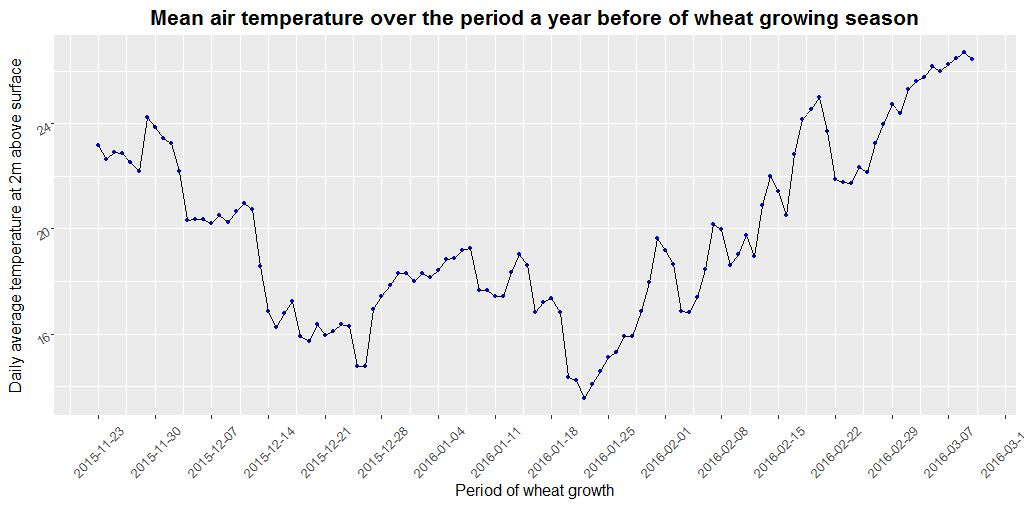
\includegraphics[width=0.9\linewidth]{../images/mean_air_temp_a_year_before} 

}

\caption{Mean air temperature 2m above surface at the site of study a year before expected wheat growing season}\label{fig:weather-previous}
\end{figure}
\setlength{\baselineskip}{1.5\baselineskip}

\hypertarget{planting-and-management}{%
\section{Planting and management}\label{planting-and-management}}

Field was sown in Nov 24, 2016. Seeds were continuously sown within a row while maintaining a between row distance of 25 cm. Seeding depth of 3-5 cm was maintained. Soil sampling (results not shown) show that the dominant soil texture type occuring in the study site is medium to heavy loamy soil. Weeding was carried out twice, first 40 days after sowing and second 70 days after sowing. Blanket recommendation of fertilizer application was followed; Initially, full dose of \(K_2O\) (60 \(kg\ ha^{-1}\)) and \(P_2O_5\) (60 \(kg\ ha^{-1}\)) were applied at the time of sowing, with Nitrogen (fed as Urea) in split doses(60 kg N \(ha^{-1}\) as basal and remaining 60 kg N \(ha^{-1}\) top dressed after irrigation). Total lengths of the field row and column were 18 \(m\) and 19.5 \(m\), respectively. Individual plots of size 0.94 \(m^2\), occupying a Total area of 351 \(m^2\) (Net Plot Area: 225 \(m^2\)) were laid in rectangular grids of regular shapes.

Irrigation was limited to once-only throughout the growing period. It is expected that the field will have ample amount of residual moisture during crops' establishment period to start with, because the site usually stays logged with water during the months of August and extended halves of September. The irrigation will be scheduled to best avoid pre-antheis moisture stress, as this has been implied in largest losses resulting in number of fertile florets and the final grain weight (Innes \& Blackwell, 1981). Water will be sourced from a deep tubewell and the field will be moistened untill saturated field condition will have been achieved.

Application of insecticidal sprays and disease checking sprays were avoided. This is to promote natural epiphytotic conditions. Observations on disease severity were mostly taken in reference to Zadok's scale of growth scoring.

\hypertarget{design-treatments-specification-and-layout}{%
\section{Design, treatments specification and layout}\label{design-treatments-specification-and-layout}}

Current study, using a small number of check varieties and sparing amounts of test entries, is adapted to fit a problem domain of early genration varietal testing applying row-column design for smaller number of checks. This allows for the estimation of design effects as spatial components, as well as for specification of custom spatial error model, if required.
\begin{itemize}
\item
  Number of rows (\(k\)): 12
\item
  Number of columns (\(s\)): 20
\item
  Number of checks (\(\nu_{\textit{c}}\)): 4
\item
  Number of rowgroups (\(g_k\)): 3
\item
  Number of colgroups (\(g_s\)): 4
\item
  Number of new entries (\(\nu_{\textit{e}}\)): 104
\item
  Number of plots allocated to checks per block (\(\nu_{g_{k}g_{s}}\)): \emph{variable}
\end{itemize}
An augmented design that accomodates \(\nu_{\textit{e}}=104\) unreplicated entries and \(\nu_{\textit{c}}=4\) replicated check cultivars with the number of rows \(\textit{k} = 12\) and the number of columns \(\textit{s} = 20\) was been generated. Each row and column is a complete block with respect to checks. A block (\(g_{k}g_{s}\)) specified by intersection of a rowgroup and a colgroup contains complete but varying number of check plots. A field layout of the the randomized design has been shown in Figure \ref{fig:augmented-layout}.
\begin{figure}

{\centering 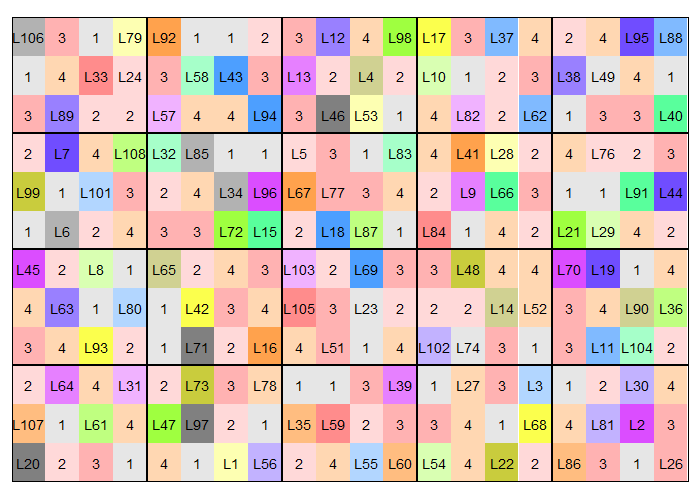
\includegraphics[width=0.9\linewidth]{../images/design_layout} 

}

\caption{Randomized layout of Augmented Row-Column Design}\label{fig:augmented-layout}
\end{figure}
\hypertarget{sampling-and-statistical-analysis}{%
\section{Sampling and statistical analysis}\label{sampling-and-statistical-analysis}}

Individual plots were sampled for making observations. At least four plant hills, except for visual scoring and making observations on plant-environment interacting response (eg. canopy temperature depression, soil temperature and soil moisture traits) where distinct protocol exists, were randomly selected and a few representative tiller from each hill were duely analysed for their relevent traits (enlisted in Table \ref{tab:yld-morph-md}).

As described earlier in Section \ref{stat-an-aug-row-col}, a mixed linear model of the form as shown (with modification), in Equation \eqref{eq:fixed-linear-model-form} was fitted for each of the response variables
\(y\). The \(genotype\) term was further partitioned to separate out Check cultivars and entries (Piepho, Williams, \& Fleck, 2006). An assumption regarding entry genotypes that these arise from a common set of germplasm and that as a whole represent all variation in a breeding population of interest was made.

All model terms except for the Check variety effects, which was considered as fixed because they are purposely selected, were expressed with random intercept terms for obtaining model parameters (Wolfinger et al., 1997). Model fitting was done through \texttt{lmer} function of \textbf{lme4} package. The model formula was fitted for obtaining REML estimates of the parameters by a single call to for both fixed and random effects terms. A general matrix structure representation in a linear mixed model with conditional distribution of \(y\) given \(\mathcal{B} =\beta\) can be represented as shown in Equation \eqref{eq:linear-mixed-form},
\begin{equation}
(y|\mathcal{B}) \approx \mathcal{N}(X\beta + Zb, \sigma^{2}W^{-1})
\label{eq:linear-mixed-form}
\end{equation}
where \(Z\) is the \(n \times q\) model matrix for the \(q\)-dimensional vector-valued random effects variable, \(\mathcal{B}\), whose value we are fixing at \(b\). The unconditional distribution of \(\mathcal{B}\) is also multivariate normal with mean zero and a parameterized \(q \times q\) variance-covariance matrix (Bates, Mächler, Bolker, \& Walker, 2015).

For multiple comparison of fixed effects means and stepwise variable selection procedure, least squares means and confidence intervals were calculated by Satterthwaite approximation of degrees of freedom (Kuznetsova, Brockhoff, \& Christensen, 2017).

Likewise, Relative Efficiency (RE) of alternative model over null model was calculated to augment the decision about model selection. Formula \eqref{eq:relative-eff} was used to compute RE.
\begin{equation}
RE = \frac{Error\ variance\ of\ Null\ Model}{Error\ variance\ of\ Alternative\ model}
\label{eq:relative-eff}
\end{equation}
All exploratory and analytical works were accomplished in ``R'' (an open source computing environment), with open source statistical packages. An extensive list of all packages used in the course of modeling and inference is provided in Appendix \ref{ii}.

\hypertarget{leaf-health}{%
\section{Leaf health assessment}\label{leaf-health}}

Leaf health trait was explained as a composite of two componenet traits- leaf greenness trait and foliar pathogen associated leaf disease score- each of which, on their own, are more readily observable phenotypic traits.

\hypertarget{greenness}{%
\subsection{Flag leaf greenness assessment}\label{greenness}}

A two approach method has been adopted to describe the SG feature. This feature was defined as:
\begin{enumerate}
\def\labelenumi{\arabic{enumi}.}
\tightlist
\item
  Leaf Area Under Greenness(LAUG) approach
\end{enumerate}
\begin{verbatim}
- difference for 0-9 visual score of green coloration (chlorophyll) of flag leaf at anthesis (Zadoks stage 65), medium milk (Zadoks stage 75) and soft dough (Zadoks stage 85) stages.
\end{verbatim}
\begin{enumerate}
\def\labelenumi{\arabic{enumi}.}
\setcounter{enumi}{1}
\tightlist
\item
  SPAD approach
\end{enumerate}
\begin{verbatim}
- difference in SPAD values(recorded at Zadoks stage 65 and 85) of flag leaf.
\end{verbatim}
The leaf greeenness scores was considered to group genotypes into classess shown in Table \ref{tab:leaf-greenness}:
\begin{table}[H]

\caption{\label{tab:leaf-greenness}Leaf greenness score intrepretation}
\centering
\begin{tabular}[t]{ll}
\toprule
\textbf{Greenness score} & \textbf{Greenness rating}\\
\midrule
 & non-green\\
 & moderately non-green\\
 & moderately green\\
 & green\\
\bottomrule
\end{tabular}
\end{table}
A similar method has been outlined by (Joshi, Chand, \& Arun, 2002) for SG trait assessment in wheat. But, current method employs emperical basis outlined in (Joshi et al., 2007) for LAUG calculation. The Leaf Area Under Greenness (LAUG) based on greenness scores over time (PLANK \& others, 1963) was estimated from the Equation \eqref{eq:laug-van-plank}
\begin{equation}
LAUG = \sum_{i = 1}^a \left [\left\{ \frac{Y_i + Y_{(i+1)}}{2}\right\} \times (t_{i+1}-t_i)\right ]
\label{eq:laug-van-plank}
\end{equation}
\hypertarget{foliar-blight-complex-associated-leaf-disease-scoring}{%
\subsection{Foliar blight complex associated leaf disease scoring}\label{foliar-blight-complex-associated-leaf-disease-scoring}}

Disease score observations of individual plots were made for foliar disease pathogens (\emph{Cochliobolus sativus}, \emph{Pyrenophora tritici-repentis}) with attributable symptoms (Duveiller \& Sharma, 2012) in a way descibed by (Saari \& Prescott, 1975). Presence of the pathogen complex was revealed upon microscopic studies, during early stage diagnostics of the disease. A image of \emph{Cochliobolus sativus} seen under the microscopic in a slide slide is shown in Figure \ref{fig:microscope-disease} as confirmatory diagnosis of foliar blight pathogen as causative agent of Foliar blight disease.. A single digit scoring system was adopted for scoring 5 random plants on each plot the flag leaf and the other directly lower to it. The score categories explaining the response to disease is interpreted in Table \ref{tab:fpa-leaf-score}.
\begin{figure}

{\centering 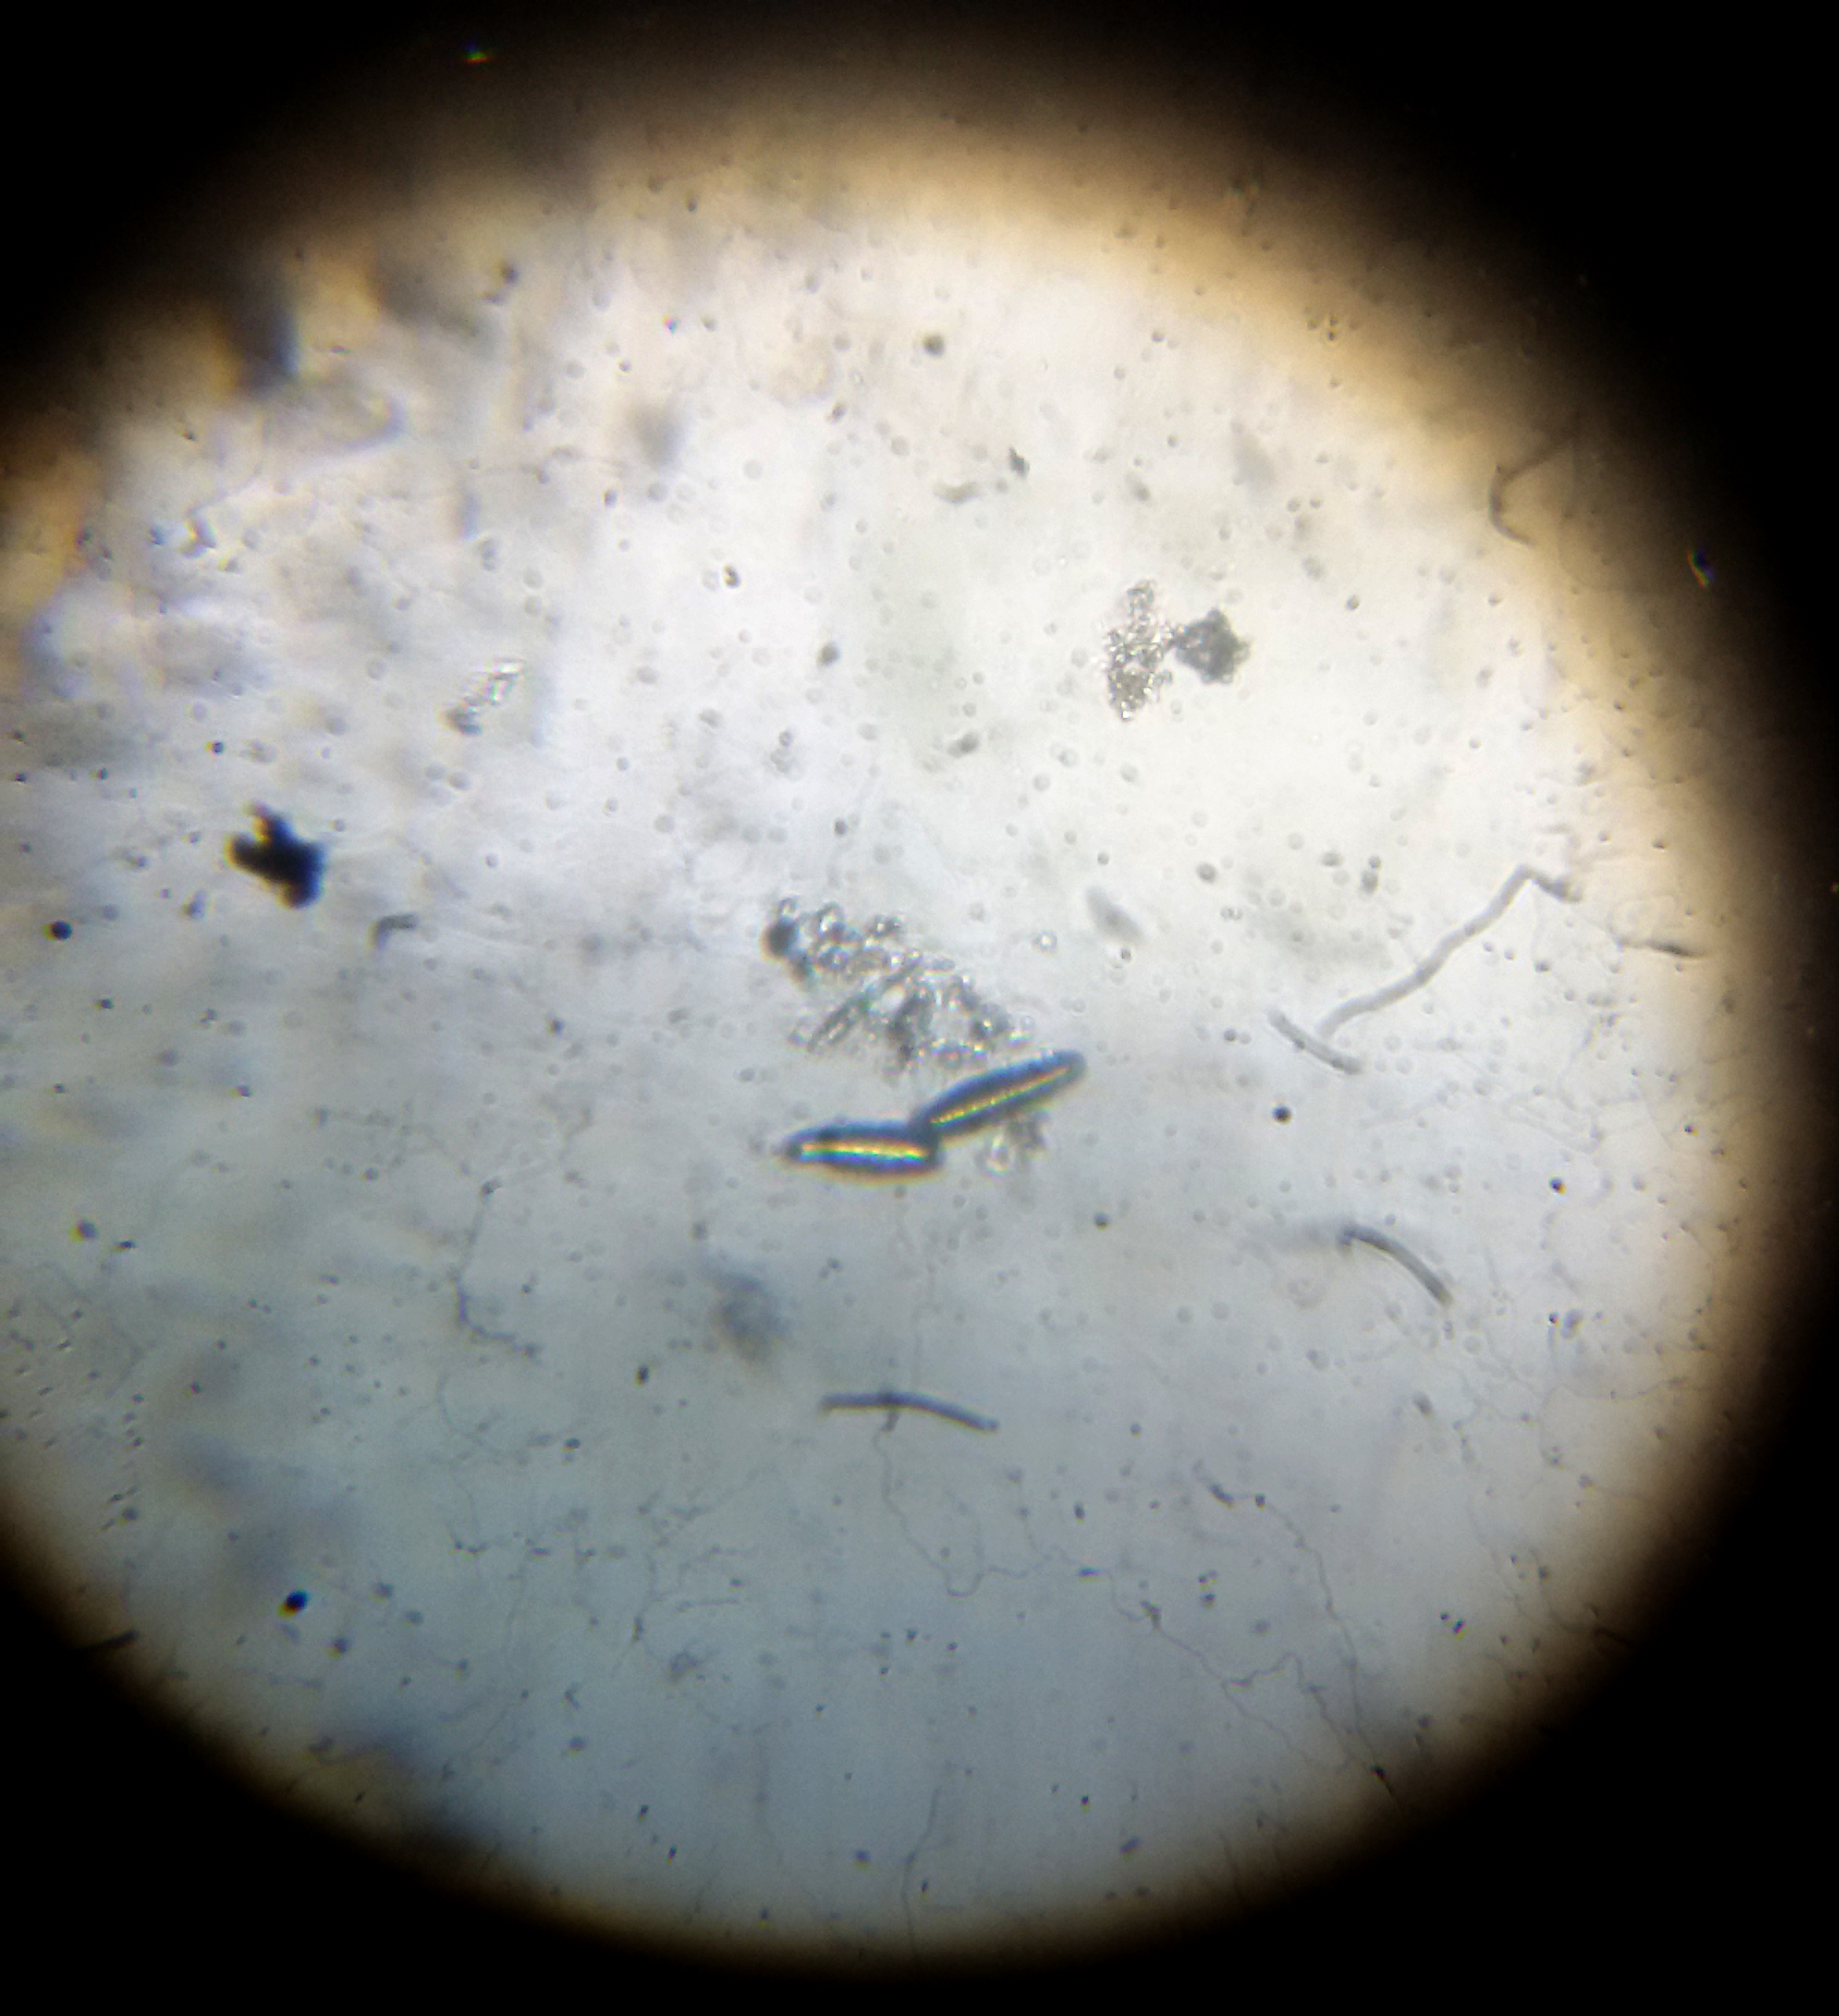
\includegraphics[width=0.8\linewidth]{../images/disease_diag/distinct_spores_20161225_114304} 

}

\caption{An image of slide under microscope showing \textit{Cochliobolus} spp.}\label{fig:microscope-disease}
\end{figure}
\begin{table}

\caption{\label{tab:fpa-leaf-score}Foliar pathogen associated disease score interpretation}
\centering
\begin{tabular}[t]{ll}
\toprule
\textbf{Disease score} & \textbf{Score rating}\\
\midrule
0-1 & very less affected\\
2-3 & less affected\\
4-5 & mildly affected\\
5-7 & mildly unaffected\\
7-8 & much affected\\
\addlinespace
8-9 & very much affected\\
\bottomrule
\end{tabular}
\end{table}
For assessing foliar pathogen associated leaf score, scoring was limited only upto Zadok's stage S77(Late milk stage). This is to acknowledge the fact that, after this stage the natural cycle of senescence confounds the effects that follow due to pathogen activity (Neupane et al., 2007).

\hypertarget{obs}{%
\section{Observation}\label{obs}}

Data were recorded from the field for the following response variables.

\hypertarget{yield-morphology-phenology-soil-and-atmospheric-conditions}{%
\subsection{Yield, morphology, phenology, soil and atmospheric conditions}\label{yield-morphology-phenology-soil-and-atmospheric-conditions}}

The record of all observations made on field, those including crops' yield, morphology, phenology traits, and fields' soil and atmospheric conditions has been shown in Table \ref{tab:yld-morph-md}.
\begin{longtable}[t]{>{\raggedright\arraybackslash}p{5.2cm}>{\raggedright\arraybackslash}p{8.2cm}}
\caption{\label{tab:yld-morph-md}Field records of crop yield, morphology, phenology, and soil and atmospheric conditions}\\
\toprule
Data & Stage recorded\\
\midrule
Vegetative growth progression & Tillering (Zadoks stage 21-29)\\
Insect foliar damage score & Tillering (Zadoks stage 21-29)\\
Soil moisture temperature and EC & Jointing and Booting (Zadoks stage 37 and 40)\\
Days to heading & when approximately 50\% of the plants in a plot are at Zadoks stage 55\\
Canopy sparseness & Heading (Zadoks stage 55)\\
\addlinespace
Leaf glaucousness & Anthesis (Zadoks 60)\\
Canopy temperature depression & Anthesis (Zadoks stage 65)\\
Flag leaf greenness rating I & Anthesis (Zadoks stage 65)\\
Soil plant analytical development & Anthesis and soft dough (Zadoks stage 65 and 85)\\
Disease score & Anthesis and Late milk (Zadoks stage 65 and 77)\\
\addlinespace
Days to anthesis & when approximately 50\% of the plants in a plot are at Zadoks stage 65\\
Leaf area & Medium milk (Zadok stage 75)\\
Plant height & Medium milk (Zadok stage 75)\\
Weed score & Medium milk (Zadok stage 75)\\
Number of effective tillers & Medium milk (Zadok stage 75)\\
\addlinespace
Flag leaf greenness rating II & Medium milk (Zadok stage 75)\\
Flag leaf greenness rating III & Soft dough (Zadoks stage 85)\\
Defective heads count & Ripening (Zadoks stage 90)\\
Panicle length & Ripening (Zadoks stage 92)\\
Days to maturity & Ripening (Zadoks stage 92)\\
\addlinespace
Number of grains per panicle & After harvested\\
Thousand kernel weight & After harvested and dried\\
Grain yield & After harvested and dried\\
\bottomrule
\end{longtable}
\hypertarget{missing-values-treatment}{%
\section{Missing values treatment}\label{missing-values-treatment}}

Missing values are largely a result of omitting improbable and extreme values due to biases in observation. In particular, two plots have been systematically left out from the observation record and further analysis because of less than optimal plant population stand. Nevertheless, mixed modeling procedure employed in inference offers fairly robust measures against such occurances (West, Welch, \& Galecki, 2014). For other procedures like correlation analysis (Shown in Table \ref{tab:plot-starred-corr}) pairwise complete data were used in computing the correlation coefficients. Similarly, in multivariate procedures such as PCA and cluster analysis, only complete cases were used in obtaining distance matrix.

\hypertarget{results}{%
\chapter{Results}\label{results}}

Observed response variables are summarised under three major aspects of a crop trait-- Yield and yield component traits, Leaf health traits and Crop morphological, phenological and architectural traits.

\hypertarget{modeling-yield-and-yield-component-traits}{%
\section{Modeling yield and yield component traits}\label{modeling-yield-and-yield-component-traits}}

\hypertarget{model-estimates-of-yield-and-yield-component-traits}{%
\subsection{Model estimates of yield and yield component traits}\label{model-estimates-of-yield-and-yield-component-traits}}
\begin{landscape}\begingroup\fontsize{8}{10}\selectfont
\begin{longtable}[t]{>{\centering\arraybackslash}p{2cm}>{\centering\arraybackslash}p{5.5cm}>{\centering\arraybackslash}p{2cm}>{\centering\arraybackslash}p{2cm}>{\centering\arraybackslash}p{2cm}>{\centering\arraybackslash}p{2cm}>{\centering\arraybackslash}p{2cm}}
\caption{\label{tab:yield-fitted-vs-observed-tab}Model adjusted genotypic mean responses of yield and yield component traits}\\
\toprule
encoding & Genotype & Yield & Effective tillers & Thousand kernel weight & Grain per panicle & Panicle length\\
\midrule
\endfirsthead
\caption[]{\label{tab:yield-fitted-vs-observed-tab}Model adjusted genotypic mean responses of yield and yield component traits \textit{(continued)}}\\
\toprule
encoding & Genotype & Yield & Effective tillers & Thousand kernel weight & Grain per panicle & Panicle length\\
\midrule
\endhead
\
\endfoot
\bottomrule
\endlastfoot
1 & Aditya & 3.02 & 26.7 & 36.3 & 27.1 & 16.3\\
2 & Bhrikuti & 3.55 & 30.2 & 37.7 & 26.8 & 16.8\\
3 & Gautam & 3.33 & 27.1 & 38.5 & 28.3 & 17.5\\
4 & Tilottama & 3.42 & 33.7 & 36.1 & 27.4 & 16.6\\
L1 & MUNAL \#1 & 4.07 & 27.0 & 35.9 & 28.8 & 16.6\\
L10 & MUNAL/3/HUW234+LR34/PRINIA//PFAU/WEAVER/4/... &  & 36.0 &  &  & 16.6\\
L101 & PFAU/MILAN/5/CHEN/AEGILOPS SQUARROSA (TAUS)/... & 3.28 & 30.0 & 43.6 & 27.7 & 16.4\\
L102 & PREMIO/5/TUI//2*SUNCO/SA1166/3/TUI/4/FINSI/... & 2.88 & 35.0 & 39.1 & 21.1 & 13.7\\
L103 & PREMIO/BAVIS &  & 47.0 &  &  & 15.0\\
L104 & CHIYAK//ND643/2*WAXWING/3/ND643/2*WAXWING &  & 30.0 &  &  & \\
L105 & BABAX/LR42//BABAX*2/4/SNI/TRAP\#1/3/KAUZ*2/... & 4.15 & 38.0 & 41.5 & 26.9 & 17.1\\
L106 & PFAU/MILAN//TROST/3/MUNAL \#1/4/PFAU/MILAN//... & 4.46 & 27.0 & 44.2 & 29.4 & 16.6\\
L107 & YUK/AE.SQUARROSA (217)//2*PANDORA & 2.51 & 30.0 & 39.4 & 22.3 & 13.8\\
L108 & SUP152*2//ND643/2*WAXWING & 3.44 & 36.0 & 41.5 & 28.1 & 12.9\\
L11 & SWSR22T.B./5/KAUZ//ALTAR 84/AOS/3/KAUZ/4/... &  & 28.0 &  &  & \\
L12 & WHEAR/VIVITSI//WHEAR/3/PANDORA & 3.68 & 33.0 & 46.5 & 30.7 & 15.7\\
L13 & WBLL1*2/KURUKU//TACUPETO F2001*2/BRAMBLING & 4.17 & 28.0 & 49.6 & 29.5 & 17.9\\
L14 & PASTOR/3/VORONA/CN079//KAUZ/4/MILAN/OTUS//.. & 2.85 & 39.0 & 33.8 & 26.9 & 15.9\\
L15 & FRANCOLIN \#1*2/ND643/2*WBLL1 & 2.84 & 35.0 & 37.7 & 24.6 & 14.7\\
L16 & KIRITATI/ 2*WBLL1/3/TAM200/PASTOR//TOBA97/4/... & 3.83 & 31.0 & 44.1 & 30.6 & 18.6\\
L17 & SUP152/KENYA SUNBIRD &  & 33.0 &  &  & 15.9\\
L18 & SUP152/KENYA SUNBIRD & 3.43 & 37.0 & 37.7 & 26.5 & 13.3\\
L19 & SUP152/KENYA SUNBIRD & 3.74 & 35.0 & 32.0 & 30.9 & 14.2\\
L2 & KACHU \#1 & 3.27 & 39.0 & 41.8 & 29.3 & 15.7\\
L20 & WBLL1*2/BRAMBLING/5/BABAX/LR42//BABAX*2/4/... &  & 26.0 &  &  & \\
L21 & ND643/2*WBLL1/3/KIRITATI//2*PRL/2*PASTOR/4/... &  & 34.0 &  &  & 16.3\\
L22 & BETTY/3/CHEN/AE.SQ//2*OPATA/4/BAVIS & 3.20 & 29.0 & 41.5 & 24.7 & 18.0\\
L23 & BAVIS/VORB/5/CROC\_1/AE.SQUARROSA(205)//... & 2.58 & 23.0 & 45.8 & 23.4 & 15.0\\
L24 & BABAX/LR42//BABAX/3/ER2000/4/NAVJ07 &  & 39.0 &  &  & 17.7\\
L26 & NING-MAI-96035/FINSI//HEILO/3/NAVJ07 &  & 26.0 &  &  & \\
L27 & WBLL1*2/BRAMBLING//TAM200/TUI/3/... &  & 39.0 &  &  & 17.1\\
L28 & KISKADEE \#1/5/KAUZ*2/MNV//KAUZ/3/MILAN/4/... & 4.10 & 47.0 & 39.8 & 22.6 & 14.9\\
L29 & MERCATO//PARUS/PASTOR &  & 31.0 &  &  & 16.5\\
L3 & KACHU/BECARD//WBLL1*2/BRAMBLING & 3.10 & 40.0 & 29.4 & 23.5 & 19.0\\
L30 & PREMIO//PARUS/PASTOR & 4.15 & 32.0 & 42.8 & 30.3 & 20.1\\
L31 & ND643/2*WBLL1//ND643/2*WAXWING & 3.81 & 37.0 & 46.9 & 23.9 & 16.3\\
L32 & ND643/2*WBLL1//ND643/2*WAXWING & 3.22 & 41.0 & 41.8 & 24.6 & 14.1\\
L33 & ND643/2*WBLL1//ND643/2*WAXWING &  & 41.0 &  &  & 16.7\\
L34 & SNB//CMH79A.955/3*CN079/3/ATTILA/4/CHEN/... &  & 32.0 &  &  & \\
L35 & KIRITATI/ 2*WBLL1/8/SHA7/ PRL/VEE\#6/ 3/ FASAN/... &  & 32.0 &  &  & 13.5\\
L36 & SERI.1B*2/3/KAUZ*2/BOW//KUZ/4/CIRCUS/5/... & 2.50 & 28.0 & 40.6 & 22.3 & 14.3\\
L37 & WHEAR/KUKUNA/3/C80.1/3*BATAVIA//2*WBLL1/4/... & 3.62 & 43.0 & 29.8 & 31.6 & 18.5\\
L38 & BAJ \#1*2/BECARD &  & 24.0 &  &  & 16.5\\
L39 & KACHU*2/MUNAL \#1 & 2.72 & 28.0 & 46.8 & 23.5 & 14.1\\
L4 & PRL/2*PASTOR/3/PFAU/WEAVER*2//CHAPIO &  & 38.0 &  &  & \\
L40 & KACHU*2/MUNAL \#1 & 3.20 & 27.0 & 36.0 & 21.8 & 14.4\\
L41 & KACHU/2*MUNAL \#1 &  & 34.0 &  &  & \\
L42 & KACHU/2*MUNAL \#1 &  & 33.0 &  &  & \\
L43 & KACHU*2/PANDORA & 4.36 & 50.0 & 48.0 & 23.5 & 17.0\\
L44 & SUP152/2*MUNAL \#1 & 2.43 & 24.0 & 47.9 & 24.0 & 13.5\\
L45 & FRNCLN*2/BECARD &  & 35.0 &  &  & 17.1\\
L46 & WBLL1* 2/BRAMBLING//SAAR/2*WAXWING/4/... &  & 39.0 &  &  & 17.1\\
L47 & CHIBIA//PRLII/CM65531/3/MISR 2*2/4/... & 3.45 & 30.0 & 42.4 & 26.5 & 15.2\\
L48 & CHIBIA//PRLII/CM65531/3/MISR 2*2/4/... &  & 27.0 &  &  & 14.3\\
L49 & WAXWING/KRONSTAD F2004//2*FRNCLN & 3.49 & 36.0 & 29.4 & 31.9 & 17.4\\
L5 & DANPHE/CHONTE & 2.42 & 33.0 & 34.6 & 21.9 & 15.5\\
L51 & MUNAL \#1/5/2*PRL/2*PASTOR/4/CHOIX/STAR/3/... &  & 27.0 &  &  & 13.3\\
L52 & MUNAL \#1/5/2*PRL/2*PASTOR/4/CHOIX/STAR/3/... & 3.07 & 30.0 & 42.4 & 23.4 & 12.3\\
L53 & MUNAL \#1/2*FRNCLN &  & 28.0 &  &  & \\
L54 & MUNAL \#1/2*FRNCLN & 2.89 & 34.0 & 36.9 & 29.2 & 17.5\\
L55 & MUNAL \#1*2//WHEAR/SOKOLL & 2.72 & 31.0 & 45.8 & 24.9 & 13.9\\
L56 & MUNAL \#1*2/KINGBIRD \#1 & 4.39 & 32.0 & 46.5 & 28.0 & 14.5\\
L57 & PRL/2*PASTOR//SUNSTATE/3/MUNAL \#1/4/OTUS//... &  & 31.0 &  &  & 15.9\\
L58 & PRL/2*PASTOR//SUNSTATE/3/MUNAL \#1/4/OTUS//... & 2.74 & 35.0 & 40.9 & 27.5 & 15.4\\
L59 & KAUZ*2/BOW//KAUZ/3/W98.6.38/5/SABUF/4/... &  & 26.0 &  &  & 16.4\\
L6 & SUP152/FRNCLN &  & 25.0 &  &  & \\
L60 & LERKE/5/KAUZ/3/MYNA/VUL//BUC/FLK/4/MILAN/6/... & 2.17 & 24.0 & 54.5 & 25.1 & 16.5\\
L61 & PASTOR/3/VORONA/CN079//KAUZ/4/MILAN/OTUS//... &  & 30.0 &  &  & 14.2\\
L62 & PASTOR/3/VORONA/CN079//KAUZ/4/MILAN/OTUS//... & 1.99 & 26.0 & 40.8 & 25.0 & 16.9\\
L63 & PFAU/MILAN//TROST/3/PBW65/2*SERI.1B*2/4/... & 2.83 & 27.0 & 37.9 & 29.3 & 18.0\\
L64 & PFAU/MILAN//TROST/3/PBW65/2*SERI.1B*2/4/... &  & 37.0 &  &  & \\
L65 & DOY1/AE.SQUARROSA (447)/3/KA/NAC//TRCH/4/... & 3.44 & 31.0 & 39.8 & 25.7 & 14.9\\
L66 & MON/IMU//ALD/PVN/3/BORL95/4/OASIS/2*BORL95/... &  & 32.0 &  &  & 16.8\\
L67 & WHEAR/SOKOLL/4/PASTOR//MILAN/KAUZ/3/BAV92 & 4.79 & 39.0 & 44.9 & 27.5 & 14.6\\
L68 & SOKOLL/WBLL1/4/D67.2/PARANA 66.270//... & 3.14 & 27.0 & 36.1 & 30.8 & 19.1\\
L69 & MILAN//PRL/2*PASTOR/4/CROC\_1/AE.SQUARROSA (2... &  & 33.0 &  &  & 17.4\\
L7 & MUU/FRNCLN & 2.40 & 25.0 & 44.9 & 26.3 & 18.9\\
L70 & TRCH/SRTU//KACHU/3/KINGBIRD \#1 & 3.58 & 28.0 & 44.6 & 23.7 & 15.8\\
L71 & TRCH/SRTU//KACHU/3/KINGBIRD \#1 & 3.98 & 47.0 & 42.7 & 22.8 & 15.2\\
L72 & TRCH/5/BAV92//IRENA/KAUZ/3/HUITES/4/DOLL &  & 26.0 &  &  & 15.6\\
L73 & BECARD \#1/3/PBW343*2/KUKUNA//PBW343*2/KUKUNA & 3.87 & 35.0 & 39.7 & 28.8 & 16.4\\
L74 & DANPHE/3/PBW343*2/KUKUNA//PBW343*2/KUKUNA & 3.28 & 27.0 & 37.1 & 24.5 & 16.0\\
L76 & PBW343*2/KUKUNA//PBW343*2/KUKUNA/6/WBLL1*2/... & 3.36 & 33.0 & 42.7 & 25.7 & 14.3\\
L77 & BECARD/6/FRET2*2/4/SNI/TRAP\#1/3/KAUZ*2/TRAP/... & 3.81 & 36.0 & 45.1 & 26.3 & 17.6\\
L78 & KACHU/6/YAR/AE.SQUARROSA (783)/4/GOV/AZ//... & 2.87 & 28.0 & 42.7 & 23.7 & 11.7\\
L79 & FRANCOLIN \#1/NELOKI & 4.12 & 37.0 & 39.4 & 31.4 & 22.1\\
L8 & PRL/ 2*PASTOR/4/CHOIX/STAR/3/HE1/3*CNO79//... & 3.90 & 28.0 &  & 21.6 & 16.3\\
L80 & PAURAQ/8/NG8201/KAUZ/4/SHA7//PRL/VEE\#6/3/... & 2.73 & 27.0 & 42.5 & 27.1 & 19.7\\
L81 & PRL/2*PASTOR//SUNSTATE/3/GRACK & 1.05 & 24.0 & 33.5 & 24.3 & 16.7\\
L82 & PICAFLOR \#1/NELOKI & 3.63 & 40.0 & 37.9 & 24.4 & 16.8\\
L83 & PICAFLOR \#1/8/NG8201/KAUZ/4/SHA7//PRL/VEE\#6/... &  & 32.0 &  &  & 15.7\\
L84 & NL971*2/MUU & 3.83 & 46.0 & 35.5 & 25.2 & 15.6\\
L85 & MUNAL \#1*2/4/HUW234+LR34/PRINIA//PBW343*2/... & 4.79 & 40.0 & 44.2 & 27.8 & 17.7\\
L86 & MUNAL \#1*2/4/HUW234+LR34/PRINIA//PBW343*2/... & 4.15 & 26.0 & 41.6 & 26.0 & 15.7\\
L87 & MUNAL \#1*2/4/HUW234+LR34/PRINIA//PBW343*2/... & 3.67 & 37.0 & 46.1 & 27.1 & 15.9\\
L88 & MUNAL \#1*2/4/HUW234+LR34/PRINIA//PBW343*2/... &  & 23.0 &  &  & 16.5\\
L89 & BECARD \#1*2/KINGBIRD \#1 &  & 41.0 &  &  & \\
L9 & DANPHE \#1*2/SHORTENED SR26 TRANSLOCATION & 3.15 & 36.0 & 34.9 & 28.9 & 16.3\\
L90 & BECARD*2/PFUNYE \#1 & 2.91 & 41.0 & 38.2 & 28.0 & 16.2\\
L91 & PBW343/PASTOR//OTUS/TOBA97*2/3/PICAFLOR \#1 & 1.27 & 28.0 & 35.1 & 24.9 & 15.9\\
L92 & ROLF07/KINGBIRD \#1//MUNAL \#1 & 4.68 & 34.0 & 38.2 & 29.2 & 16.4\\
L93 & MUNAL \#1/3/PBW343*2/KUKUNA*2//YANAC & 4.83 & 30.0 & 43.1 & 26.2 & 15.3\\
L94 & SERI.1B*2/3/KAUZ*2/BOW/KAUZ/4/PBW343*2/... & 2.07 & 37.0 & 27.0 & 24.2 & 15.4\\
L95 & KAUZ//ALTAR 84/AOS/3/MILAN/KAUZ/4/SAUAL/5/... &  & 28.0 &  &  & 15.4\\
L96 & PBW343*2/KHVAKI//PARUS/3/PBW343/PASTOR/5/... & 1.88 & 18.0 & 37.1 & 22.7 & 15.5\\
L97 & FRET2*2/4/SNI/TRAP\#1/3/KAUZ*2-TRAP//KAUZ*2/... & 1.46 & 27.0 & 32.5 & 26.4 & 15.9\\
L98 & ATTILA*2/PBW65*2//JUCHI/3/KINGBIRD \#1/4/... &  & 27.0 &  &  & 19.5\\
L99 & MUNAL \#1*2//WBLL1*2/BRAMBLING & 3.63 & 36.0 & 49.3 & 25.7 & 15.1\\*
\end{longtable}
\endgroup{}
\end{landscape}
\blandscape

\hypertarget{mixed-model-summary-of-fixed-effects-terms-of-yield-and-yield-component-traits}{%
\subsection{Mixed model summary of fixed effects terms of yield and yield component traits}\label{mixed-model-summary-of-fixed-effects-terms-of-yield-and-yield-component-traits}}

\begingroup 
\small 
\begin{longtable}{@{\extracolsep{1pt}}lccccc} 
\\[-1.8ex]\hline 
\hline \\[-1.8ex] 
 & \multicolumn{5}{c}{\textit{Dependent variable:}} \\ 
\cline{2-6} 
\\[-1.8ex] & \multicolumn{5}{c}{\textit{linear}} \\ 
 & \multicolumn{5}{c}{\textit{mixed-effects}} \\ 
 & Yield & \parbox[t]{2.5cm}{Number of effective tillers} & \parbox[t]{2.5cm}{Thousand kernel weight} & \parbox[t]{2.5cm}{Grains per panicle} & Panicle length \\ 
\\[-1.8ex] & (1) & (2) & (3) & (4) & (5)\\ 
\hline \\[-1.8ex] 
 Bhrikuti & 0.52$^{***}$ (0.14) & 3.34$^{**}$ (1.35) & 1.17 (0.85) & $-$0.22 (0.49) & 0.51 (0.33) \\ 
  & p = 0.0003 & p = 0.02 & p = 0.17 & p = 0.66 & p = 0.13 \\ 
  Gautam & 0.31$^{**}$ (0.14) & 0.33 (1.36) & 2.06$^{**}$ (0.85) & 1.33$^{***}$ (0.49) & 1.22$^{***}$ (0.33) \\ 
  & p = 0.03 & p = 0.81 & p = 0.02 & p = 0.01 & p = 0.0003 \\ 
  Tilottama & 0.40$^{***}$ (0.14) & 6.94$^{***}$ (1.36) & $-$0.32 (0.85) & 0.38 (0.49) & 0.27 (0.33) \\ 
  & p = 0.005 & p = 0.0000 & p = 0.72 & p = 0.45 & p = 0.43 \\ 
  Aditaya (Constant) & 3.02$^{***}$ (0.61) & 26.80$^{***}$ (2.45) & 36.40$^{***}$ (4.32) & 27.00$^{***}$ (1.88) & 16.30$^{***}$ (1.09) \\ 
  & p = 0.0000 & p = 0.00 & p = 0.00 & p = 0.00 & p = 0.00 \\ 
 \hline \\[-1.8ex] 
Observations & 202 & 238 & 201 & 202 & 226 \\ 
Log Likelihood & $-$209.00 & $-$752.00 & $-$575.00 & $-$452.00 & $-$414.00 \\ 
Akaike Inf. Crit. & 443.00 & 1,528.00 & 1,174.00 & 928.00 & 853.00 \\ 
Bayesian Inf. Crit. & 482.00 & 1,570.00 & 1,213.00 & 968.00 & 894.00 \\ 
\hline 
\hline \\[-1.8ex] 
\textit{Note:}  & \multicolumn{5}{r}{$^{*}$p$<$0.1; $^{**}$p$<$0.05; $^{***}$p$<$0.01} \\ 
\end{longtable} 
\endgroup

\elandscape

\hypertarget{yield}{%
\subsubsection{Yield}\label{yield}}

Genotypes show highly significant differences for the yield trait. The model with both genotypes (checks and entries) outperforms in comparison to the one without in predicting the real yield (\(\chi^2 = 14.4\) with \(df = 4\)).

Pairwise comparison of fixed effects estimate indicate that check variety Aditya has the lowest yield amongst all varieties while other have similar yields. Average yield of the lowest yielder is \(4.53\ tons\ ha^{-1}\ (\pm\ 0.60)\) and Bhrikuti yields the highest with average yield of \(5.04\ tons\ ha^{-1}\ (\pm\ 0.60)\).

Similarly, entry genotypes show considerable amount of heritable variation as evident from a large measure of variance in random effects term. ANOVA table (\ref{tab:lrt-yield}) and the dotplot (Figure \ref{fig:yield-dotplot1}) showing random effects estimates of the entry genotypes illustrate the relationship. Blocking structure, however, do not result in improvement of the effect estimates of the genotypes; blocking factors do not have significant effect on the yield trait.
\begin{table}[H]

\caption{\label{tab:yield-meanconf-tab}Mean differences in Yield of check varieties (post-hoc comparison using Tukey procedure)}
\centering
\begin{tabular}[t]{cccccccc}
\toprule
Contrast & Estimate & Std. Error & df & t value & lower & upper & Pr(>|t|)\\
\midrule
Aditya-Bhrikuti & -0.516 & 0.139 & 101.0 & -3.713 & -0.792 & -0.240 & 0.000\\
Aditya-Gautam & -0.305 & 0.140 & 99.9 & -2.179 & -0.583 & -0.027 & 0.032\\
Aditya-Tilottama & -0.400 & 0.140 & 98.8 & -2.860 & -0.677 & -0.122 & 0.005\\
Bhrikuti-Gautam & 0.211 & 0.140 & 99.9 & 1.510 & -0.066 & 0.489 & 0.134\\
Bhrikuti-Tilottama & 0.116 & 0.140 & 99.0 & 0.833 & -0.161 & 0.394 & 0.407\\
Gautam-Tilottama & -0.095 & 0.141 & 99.8 & -0.672 & -0.374 & 0.185 & 0.503\\
\bottomrule
\end{tabular}
\end{table}
\hypertarget{number-of-effective-tillers}{%
\subsubsection{Number of effective tillers}\label{number-of-effective-tillers}}

Genotypes show highly significant differences for the Number of effective tillers trait. LRT shows that both checks and entries possess heritable variation that could potentially be exploited in further selection of the germplasm. The model comparison indicates a lower BIC value and \(\chi^2\) statistic of \(35.2\) with \(4\ df\).

Pairwise comparison of fixed effects estimate indicate that except for Aditya and Gautam varieties, which are similar in Number of effective tillers, all other check varieties differ for the trait. Highest number of effective tillers was found in Tilottama (\(33.73\ \pm\ 2.46\)) and the least in Aditya (\(26.80\ \pm\ 2.45\)) varieties.

In contrast, entry genotypes are not significantly different for the variability they contribute in the number of effective tillers. This can be seen as small spread in genotype estimates of the random effects term. ANOVA table (\ref{tab:lrt-netill}) and the dotplot (Figure \ref{fig:yield-dotplot2}) showing random effects estimates of the entry genotypes illustrate the relationship. None of the blocking components might add to the benefit of improving the estimates of the genotypic effects for the number of effective tillers trait (based on LRT).
\begin{table}[H]

\caption{\label{tab:yield-meanconf-tab2}Mean differences in Number of effective tillers of check varieties (post-hoc comparison using Tukey procedure)}
\centering
\begin{tabular}[t]{cccccccc}
\toprule
Contrast & Estimate & Std. Error & df & t value & lower & upper & Pr(>|t|)\\
\midrule
Aditya-Bhrikuti & -3.339 & 1.35 & 121 & -2.471 & -6.015 & -0.664 & 0.015\\
Aditya-Gautam & -0.328 & 1.36 & 121 & -0.241 & -3.026 & 2.369 & 0.810\\
Aditya-Tilottama & -6.939 & 1.36 & 121 & -5.094 & -9.637 & -4.242 & 0.000\\
Bhrikuti-Gautam & 3.011 & 1.36 & 120 & 2.212 & 0.316 & 5.707 & 0.029\\
Bhrikuti-Tilottama & -3.600 & 1.36 & 120 & -2.646 & -6.293 & -0.906 & 0.009\\
Gautam-Tilottama & -6.611 & 1.37 & 120 & -4.822 & -9.326 & -3.897 & 0.000\\
\bottomrule
\end{tabular}
\end{table}
\hypertarget{thousand-kernel-weight}{%
\subsubsection{Thousand kernel weight}\label{thousand-kernel-weight}}

Genotypes are significantly different (at \(p = 0.05\)) for the Thousand kernel weight trait. LRT shows that trait variation has the genetic roots linked to the genotype (for both checks and entries). Relative advantage of including genotype in the model terms is also highlighted by a lower BIC value and \(\chi^2\) statistic of \(10.279\) with \(4\ df\).

Pairwise comparison of fixed effects estimate indicate that Gautam variety has the highest thousand kernel weight (\(38.48\ \pm\ 4.32\) gm) and Tilottama has the least (\(36.103\ \pm\ 4.32\) gm) among check varieties.

Likewise, entry genotypes possessing a considerable amount of heritable variation can be evident from the ANOVA table (\ref{tab:lrt-tkw}) and the dotplot (Figure \ref{fig:yield-dotplot3} showing random effects estimates of the entry genotypes illustrate the relationship. Besides genotype, blocking along the columns nested inside the column groups had a significant role in determination of Thousand kernel weight.
\begin{table}[H]

\caption{\label{tab:yield-meanconf-tab3}Mean differences in Thousand kernel weight of check varieties (post-hoc comparison using Tukey procedure)}
\centering
\begin{tabular}[t]{cccccccc}
\toprule
Contrast & Estimate & Std. Error & df & t value & lower & upper & Pr(>|t|)\\
\midrule
Aditya-Bhrikuti & -1.170 & 0.847 & 90.6 & -1.381 & -2.853 & 0.513 & 0.171\\
Aditya-Gautam & -2.064 & 0.853 & 90.1 & -2.419 & -3.759 & -0.369 & 0.018\\
Aditya-Tilottama & 0.316 & 0.852 & 89.2 & 0.371 & -1.377 & 2.009 & 0.712\\
Bhrikuti-Gautam & -0.894 & 0.852 & 89.9 & -1.049 & -2.588 & 0.799 & 0.297\\
Bhrikuti-Tilottama & 1.486 & 0.851 & 89.1 & 1.747 & -0.205 & 3.176 & 0.084\\
Gautam-Tilottama & 2.380 & 0.858 & 89.8 & 2.773 & 0.675 & 4.085 & 0.007\\
\bottomrule
\end{tabular}
\end{table}
\hypertarget{number-of-grains-per-panicle}{%
\subsubsection{Number of grains per panicle}\label{number-of-grains-per-panicle}}

Genotypes show significant differences for the Number of grains per panicle trait. LRT shows that both checks and entries possess significant (\(\chi^2\) statistic=\(11.59\) with \(4\ df\)) heritable variation.

Pairwise comparison of fixed effects estimate indicate that check varieties Aditya and Gautam have different mean Number of grains per panicle. Likewise pairwise contrast using same procedure (Tukey) indicates different means for Bhrikuti and Gautam varieties. The highest and the lowest number of grains per panicle was found in Gautam (\(28.36\ \pm\ 1.88\)) and Bhrikuti (\(26.80\ \pm\ 1.88\)) varieties, respectively.

Similarly, entry genotypes show considerable amount of heritable variation as evident from a large measure of variance in random effects term. ANOVA table (\ref{tab:lrt-gperpan}) and the dotplot (Figure \ref{fig:yield-dotplot4}) showing random effects estimates of the entry genotypes illustrate the relationship. Likewise, no significant effects were associated with either of the blocking factors.
\begin{table}[H]

\caption{\label{tab:yield-meanconf-tab4}Mean differences in Number of grains per panicle of check varieties (post-hoc comparison using Tukey procedure)}
\centering
\begin{tabular}[t]{cccccccc}
\toprule
Contrast & Estimate & Std. Error & df & t value & lower & upper & Pr(>|t|)\\
\midrule
Aditya-Bhrikuti & 0.221 & 0.488 & 120 & 0.453 & -0.745 & 1.187 & 0.651\\
Aditya-Gautam & -1.331 & 0.492 & 121 & -2.703 & -2.305 & -0.356 & 0.008\\
Aditya-Tilottama & -0.377 & 0.492 & 121 & -0.765 & -1.351 & 0.598 & 0.446\\
Bhrikuti-Gautam & -1.552 & 0.492 & 121 & -3.155 & -2.525 & -0.578 & 0.002\\
Bhrikuti-Tilottama & -0.598 & 0.491 & 120 & -1.216 & -1.571 & 0.375 & 0.226\\
Gautam-Tilottama & 0.954 & 0.496 & 121 & 1.925 & -0.027 & 1.935 & 0.057\\
\bottomrule
\end{tabular}
\end{table}
\hypertarget{panicle-length}{%
\subsubsection{Panicle length}\label{panicle-length}}

Genotypes show highly significant differences for the panicle length trait. LRT shows that both checks and entries possess significant (\(\chi^2\) statistic=\(14.62\) with \(4\ df\)) heritable variation.

Pairwise comparison of fixed effects estimate indicate that check variety Gautam has significantly longer panicles than (all) Aditya, Tilottama and Bhrikuti. Likewise pairwise contrast using same procedure (Tukey) indicates that no difference exists between other varieties. Longest panicles were found in Gautam (\(17.53\ \pm\ 1.09\)cm) and the shortest in Aditya (\(16.32\ \pm\ 1.09\)cm) varieties.

Similarly, entry genotypes show considerable amount of heritable variation as evident from a large measure of variance in random effects term. ANOVA table (\ref{tab:lrt-panlen}) and the dotplot (Figure \ref{fig:yield-dotplot2}) showing random effects estimates of the entry genotypes illustrate the relationship. No attributable blocking effects, based on LRT, can be inferred about for the panicle length trait, alike most other yield and yield component traits.
\begin{table}[H]

\caption{\label{tab:yield-meanconf-tab5}Mean differences in Panicle length of check varieties (post-hoc comparison using Tukey procedure)}
\centering
\begin{tabular}[t]{cccccccc}
\toprule
Contrast & Estimate & Std. Error & df & t value & lower & upper & Pr(>|t|)\\
\midrule
Aditya-Bhrikuti & -0.510 & 0.331 & 129 & -1.539 & -1.165 & 0.145 & 0.126\\
Aditya-Gautam & -1.215 & 0.334 & 129 & -3.640 & -1.876 & -0.555 & 0.000\\
Aditya-Tilottama & -0.266 & 0.334 & 129 & -0.797 & -0.926 & 0.394 & 0.427\\
Bhrikuti-Gautam & -0.705 & 0.334 & 129 & -2.114 & -1.366 & -0.045 & 0.036\\
Bhrikuti-Tilottama & 0.244 & 0.334 & 129 & 0.731 & -0.416 & 0.904 & 0.466\\
Gautam-Tilottama & 0.949 & 0.336 & 129 & 2.825 & 0.284 & 1.614 & 0.005\\
\bottomrule
\end{tabular}
\end{table}
\hypertarget{mean-comparison-of-yield-and-yield-component-traits-of-entry-genotypes}{%
\subsection{Mean comparison of yield and yield component traits of entry genotypes}\label{mean-comparison-of-yield-and-yield-component-traits-of-entry-genotypes}}
\begin{figure}[H]

{\centering \subfloat[Yield\label{fig:yield-blup-viz-1}]{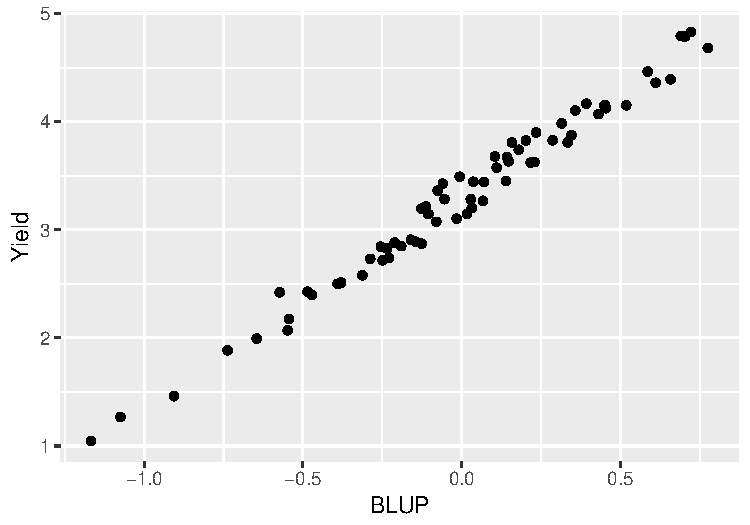
\includegraphics[width=.48\linewidth]{thesis_files/figure-latex/yield-blup-viz-1} }\subfloat[Number of effective tillers\label{fig:yield-blup-viz-2}]{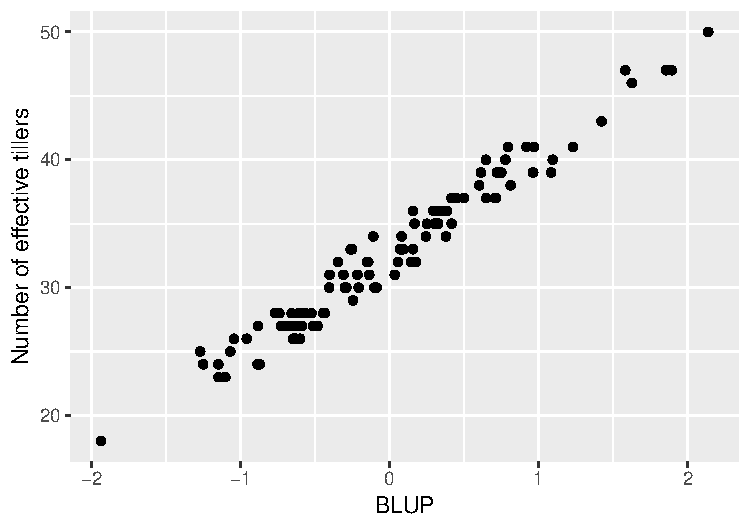
\includegraphics[width=.48\linewidth]{thesis_files/figure-latex/yield-blup-viz-2} }\newline\subfloat[Thousand kernel weight\label{fig:yield-blup-viz-3}]{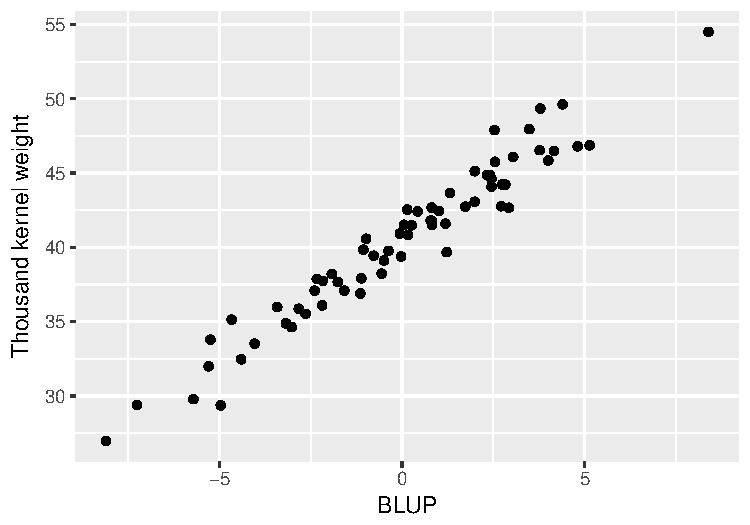
\includegraphics[width=.48\linewidth]{thesis_files/figure-latex/yield-blup-viz-3} }\subfloat[Number of grains per panicle\label{fig:yield-blup-viz-4}]{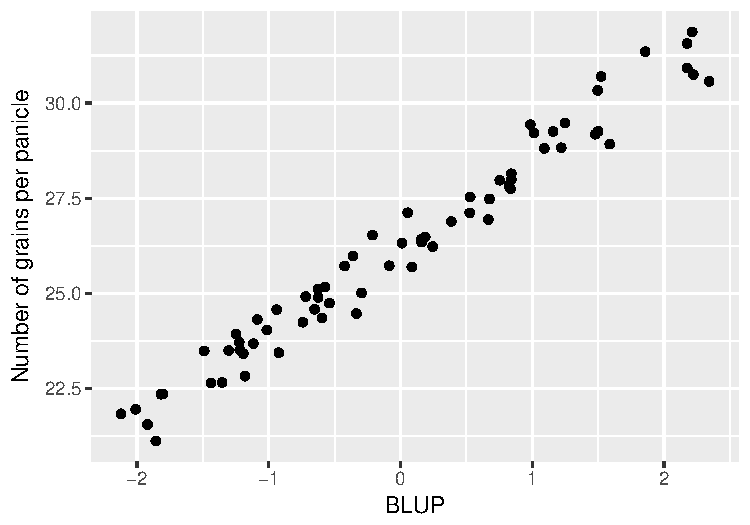
\includegraphics[width=.48\linewidth]{thesis_files/figure-latex/yield-blup-viz-4} }\newline\subfloat[Panicle length\label{fig:yield-blup-viz-5}]{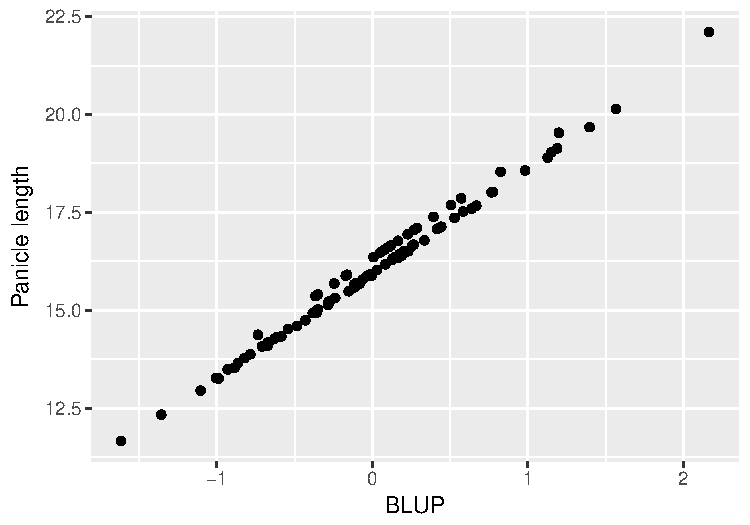
\includegraphics[width=.48\linewidth]{thesis_files/figure-latex/yield-blup-viz-5} }

}

\caption{Scatterplot of observed versus BLUP values of yield and yield component traits}\label{fig:yield-blup-viz}
\end{figure}
Scatterplot showing observed mean values of yield and yield component traits plotted against their respective genotypic BLUP values is presented in Figure \ref{fig:yield-blup-viz}.

The coefficient of determination, as computed by squared correlation coefficient between the observed and fitted values of random effects model are 0.61, 0.36, 0.71, 0.55, 0.48, respectively for the Yield, Number of effective tillers, Thousand kernel weight, Number of grains per panicle and Panicle length.
\begin{figure}[H]

{\centering \subfloat[Yield\label{fig:yield-dotplot-1}]{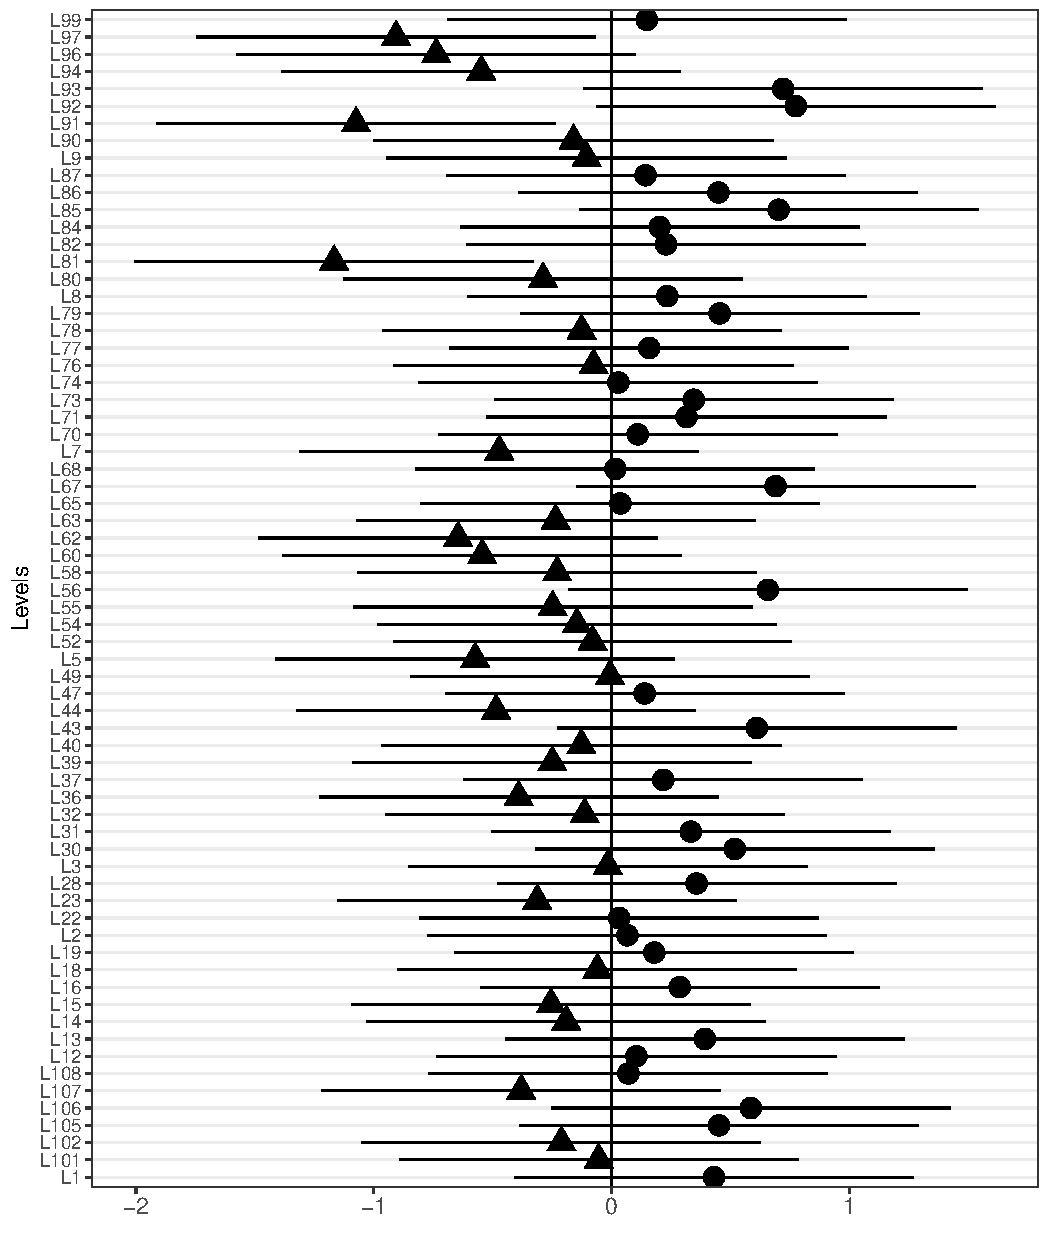
\includegraphics[width=.48\linewidth]{thesis_files/figure-latex/yield-dotplot-1} }\subfloat[Number of effective tillers\label{fig:yield-dotplot-2}]{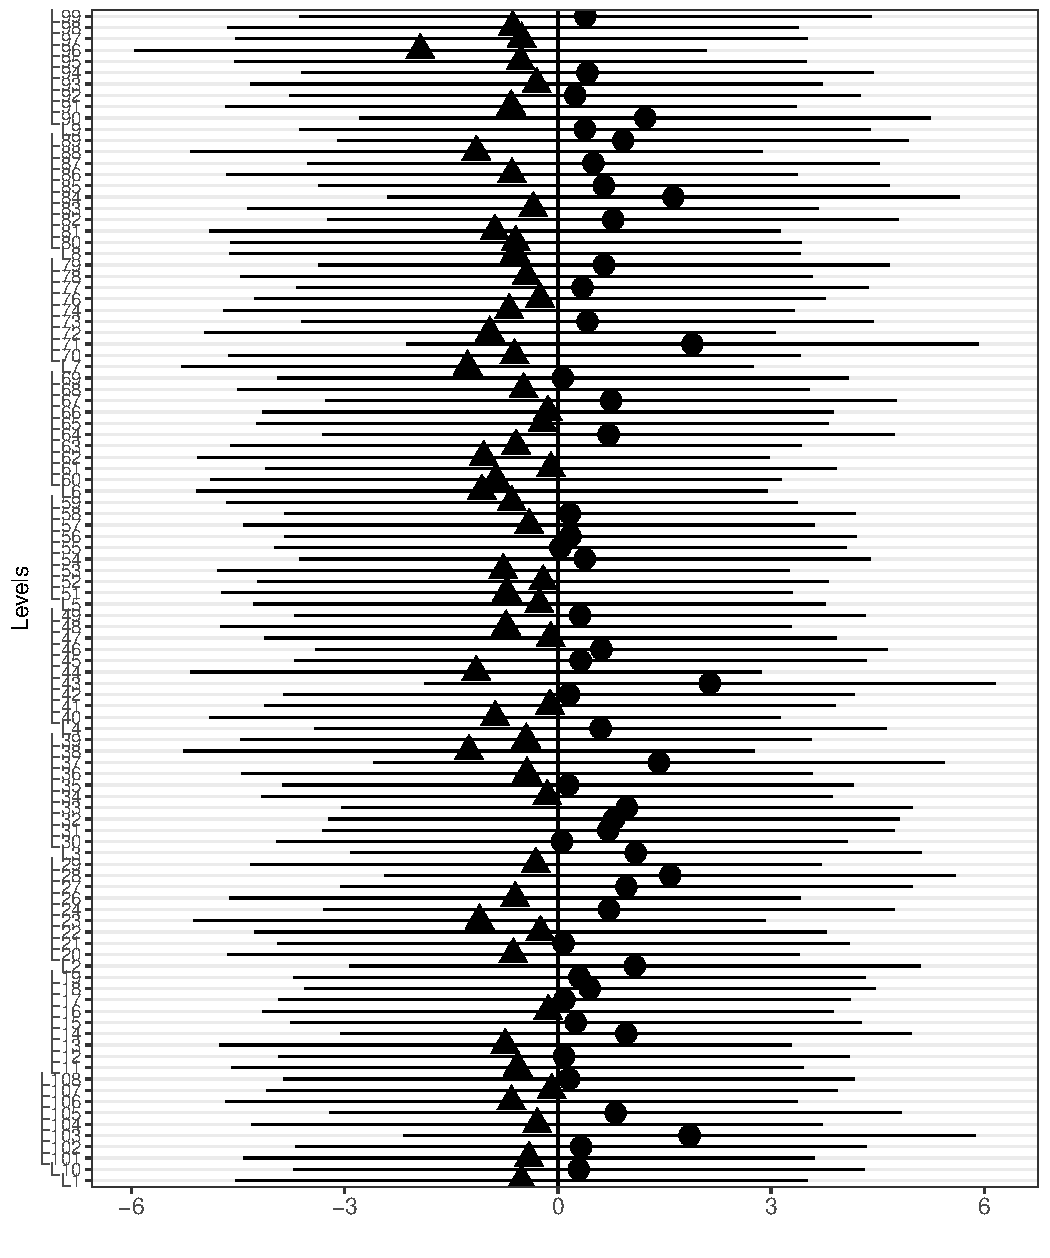
\includegraphics[width=.48\linewidth]{thesis_files/figure-latex/yield-dotplot-2} }\newline\subfloat[Thousand kernel weight\label{fig:yield-dotplot-3}]{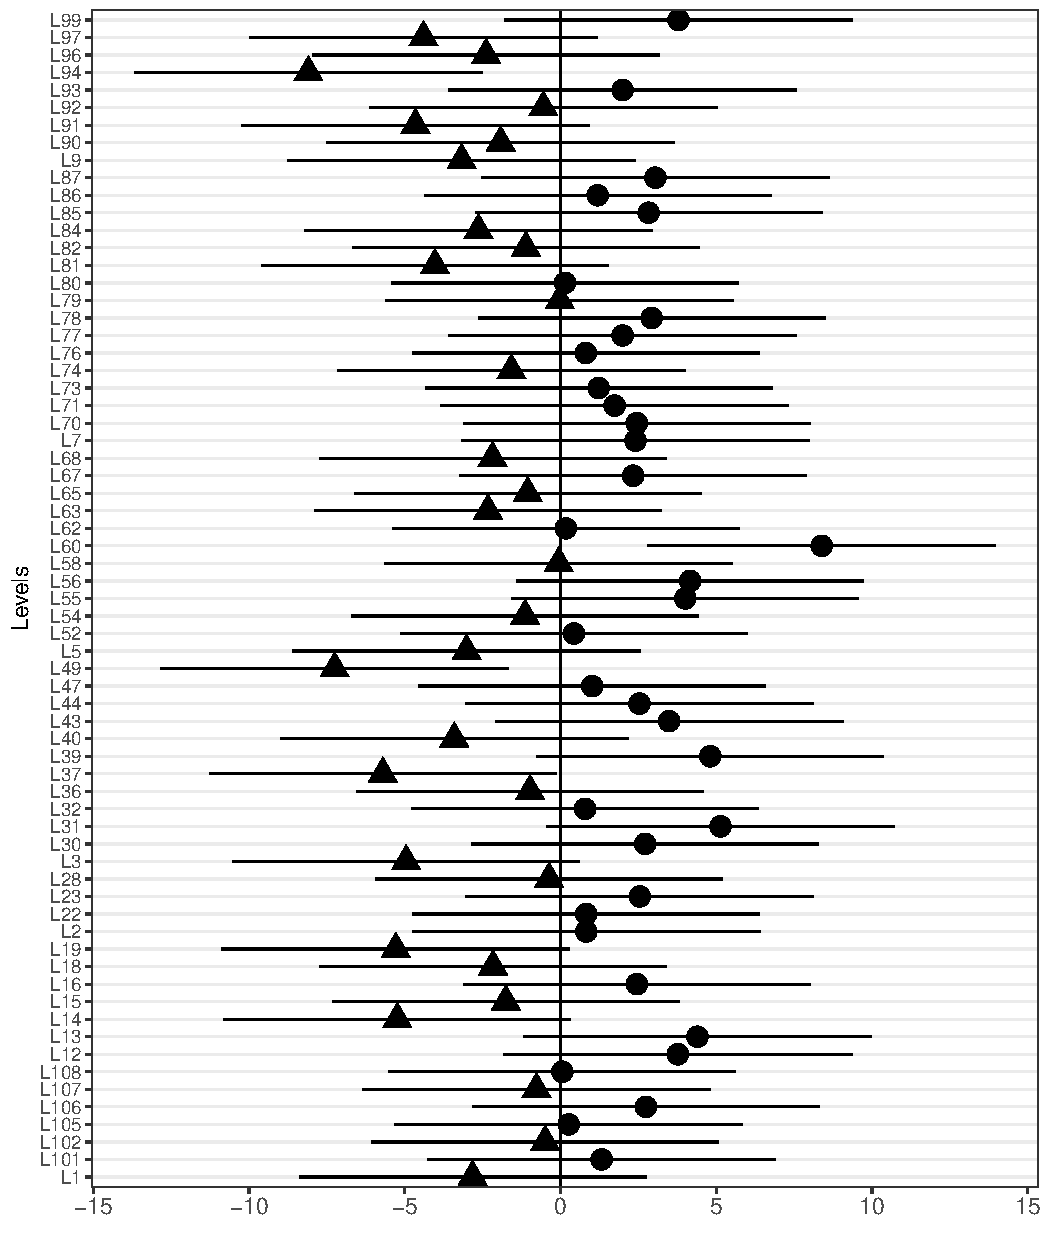
\includegraphics[width=.48\linewidth]{thesis_files/figure-latex/yield-dotplot-3} }\subfloat[Number of grains per panicle\label{fig:yield-dotplot-4}]{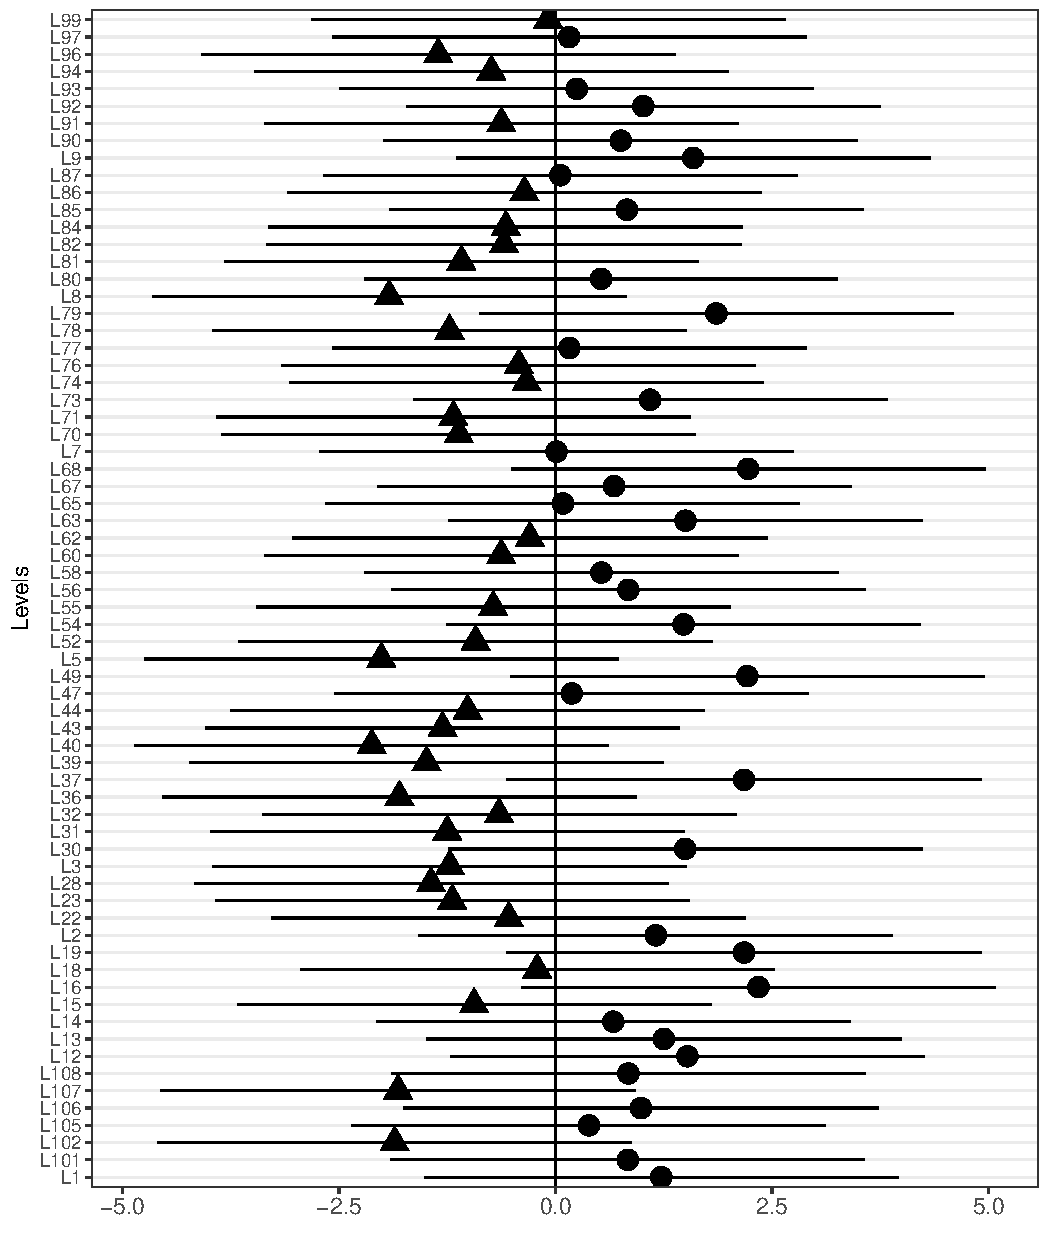
\includegraphics[width=.48\linewidth]{thesis_files/figure-latex/yield-dotplot-4} }

}

\caption{Random effect estimates of yield and yield component traits of entry genotypes}\label{fig:yield-dotplot}
\end{figure}
\begin{figure}[H]

{\centering 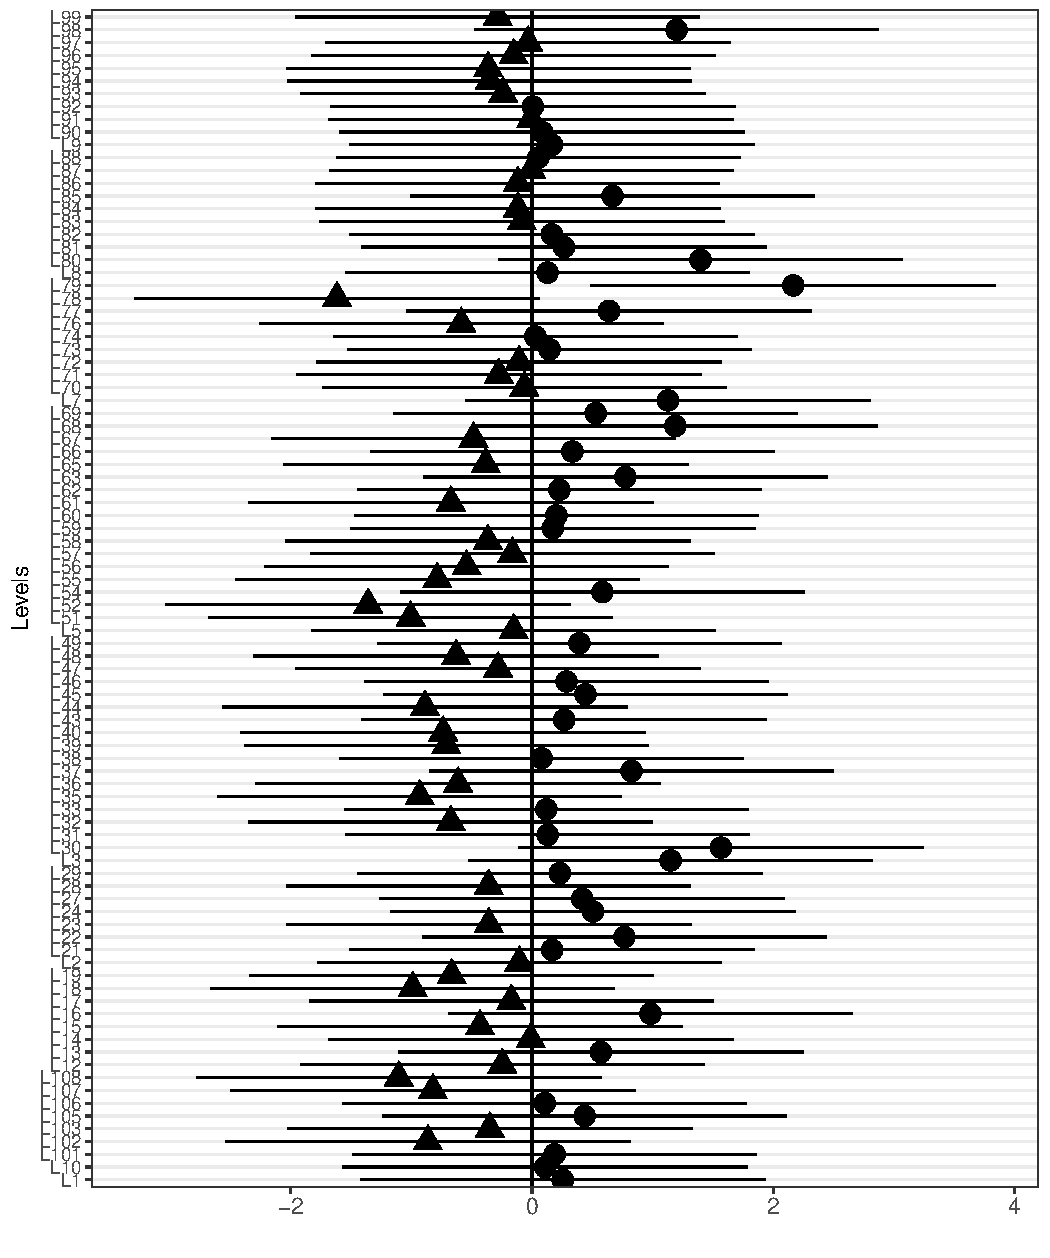
\includegraphics[width=.48\linewidth]{thesis_files/figure-latex/yield-dotplot2-1} 

}

\caption{Random effect estimates of yield and yield component traits of entry genotypes (...continued)}\label{fig:yield-dotplot2}
\end{figure}
\clearpage

\hypertarget{modeling-leaf-health-traits}{%
\section{Modeling leaf health traits}\label{modeling-leaf-health-traits}}

\hypertarget{model-estimates-of-leaf-health-traits}{%
\subsection{Model estimates of leaf health traits}\label{model-estimates-of-leaf-health-traits}}
\begin{landscape}\begingroup\fontsize{8}{10}\selectfont
\begin{longtable}[t]{>{\centering\arraybackslash}p{1.5cm}>{\centering\arraybackslash}p{4.85cm}>{\centering\arraybackslash}p{1.75cm}>{\centering\arraybackslash}p{1.75cm}>{\centering\arraybackslash}p{1.75cm}>{\centering\arraybackslash}p{1.75cm}>{\centering\arraybackslash}p{1.75cm}>{\centering\arraybackslash}p{1.75cm}}
\caption{\label{tab:leaf-health-fitted-vs-observed-tab}Model adjusted genotypic mean responses of leaf health traits}\\
\toprule
encoding & Genotype & Disease (Zadok's 75) & Greenness (Zadok's 65) & Greenness (Zadok's 75) & Greenness (Zadok's 85) & LAUG (Zadok's 65-75) & LAUG (Zadok's 75-85)\\
\midrule
\endfirsthead
\caption[]{\label{tab:leaf-health-fitted-vs-observed-tab}Model adjusted genotypic mean responses of leaf health traits \textit{(continued)}}\\
\toprule
encoding & Genotype & Disease (Zadok's 75) & Greenness (Zadok's 65) & Greenness (Zadok's 75) & Greenness (Zadok's 85) & LAUG (Zadok's 65-75) & LAUG (Zadok's 75-85)\\
\midrule
\endhead
\
\endfoot
\bottomrule
\endlastfoot
1 & Aditya & 2.86 & 8.07 & 7.33 & 5.83 & 110.8 & 92.89\\
2 & Bhrikuti & 3.32 & 8.01 & 6.66 & 5.20 & 108.4 & 86.28\\
3 & Gautam & 2.45 & 7.92 & 7.18 & 5.14 & 109.8 & 84.78\\
4 & Tilottama & 3.36 & 7.95 & 6.51 & 4.89 & 107.2 & 77.56\\
L1 & MUNAL \#1 & 4.00 & 8.13 & 5.63 & 5.42 & 111.3 & 68.27\\
L10 & MUNAL/3/HUW234+LR34/PRINIA//PFAU/WEAVER/4/... & 3.00 & 8.84 & 3.98 & 3.53 & 101.3 & 56.60\\
L101 & PFAU/MILAN/5/CHEN/AEGILOPS SQUARROSA (TAUS)/... & 2.00 & 8.84 & 4.89 & 4.68 & 93.2 & 47.19\\
L102 & PREMIO/5/TUI//2*SUNCO/SA1166/3/TUI/4/FINSI/... & 4.00 & 8.75 & 7.01 & 6.52 & 103.2 & 95.55\\
L103 & PREMIO/BAVIS & 2.50 & 7.73 & 5.81 & 3.98 & 99.6 & 55.47\\
L104 & CHIYAK//ND643/2*WAXWING/3/ND643/2*WAXWING & 6.00 & 7.45 & 3.43 & 0.65 & 83.5 & 30.94\\
L105 & BABAX/LR42//BABAX*2/4/SNI/TRAP\#1/3/KAUZ*2/... & 4.50 & 7.80 & 5.41 & 4.21 & 104.6 & 65.47\\
L106 & PFAU/MILAN//TROST/3/MUNAL \#1/4/PFAU/MILAN//... & 1.33 & 8.35 & 7.96 & 6.97 & 120.1 & 92.18\\
L107 & YUK/AE.SQUARROSA (217)//2*PANDORA & 6.00 & 7.92 & 6.36 & 5.01 & 102.7 & 92.90\\
L108 & SUP152*2//ND643/2*WAXWING & 4.00 & 8.84 & 4.06 & 4.02 & 100.4 & 42.28\\
L11 & SWSR22T.B./5/KAUZ//ALTAR 84/AOS/3/KAUZ/4/... & 2.00 & 8.84 & 5.97 & 6.06 & 113.1 & 86.15\\
L12 & WHEAR/VIVITSI//WHEAR/3/PANDORA & 1.00 & 7.86 & 4.46 & 3.34 & 98.2 & 53.31\\
L13 & WBLL1*2/KURUKU//TACUPETO F2001*2/BRAMBLING & 1.50 & 7.79 & 7.56 & 5.17 & 113.3 & 98.78\\
L14 & PASTOR/3/VORONA/CN079//KAUZ/4/MILAN/OTUS//.. & 4.00 & 8.60 & 5.77 & 5.51 & 107.2 & 72.10\\
L15 & FRANCOLIN \#1*2/ND643/2*WBLL1 & 3.50 & 8.67 & 4.23 & 3.97 & 90.3 & 60.03\\
L16 & KIRITATI/ 2*WBLL1/3/TAM200/PASTOR//TOBA97/4/... & 5.00 & 8.10 & 5.01 & 4.04 & 94.2 & 63.07\\
L17 & SUP152/KENYA SUNBIRD & 2.00 & 7.23 & 4.77 & 0.94 & 90.5 & 20.16\\
L18 & SUP152/KENYA SUNBIRD & 5.50 & 8.67 & 3.19 & 1.64 & 82.8 & 32.26\\
L19 & SUP152/KENYA SUNBIRD & 2.50 & 8.00 & 3.83 & 2.26 & 88.7 & 32.11\\
L2 & KACHU \#1 & 7.00 & 7.77 & 7.48 & 4.43 & 110.5 & 86.48\\
L20 & WBLL1*2/BRAMBLING/5/BABAX/LR42//BABAX*2/4/... & 6.00 & 8.59 & 5.77 & 5.56 & 112.9 & 78.65\\
L21 & ND643/2*WBLL1/3/KIRITATI//2*PRL/2*PASTOR/4/... & 2.00 & 8.49 & 6.49 & 6.31 & 111.9 & 85.33\\
L22 & BETTY/3/CHEN/AE.SQ//2*OPATA/4/BAVIS & 7.00 & 8.13 & 4.77 & 4.49 & 103.8 & 58.23\\
L23 & BAVIS/VORB/5/CROC\_1/AE.SQUARROSA(205)//... & 6.00 & 7.50 & 1.84 & 0.57 & 62.6 & 9.13\\
L24 & BABAX/LR42//BABAX/3/ER2000/4/NAVJ07 & 1.50 & 8.67 & 4.03 & 3.73 & 92.4 & 42.57\\
L26 & NING-MAI-96035/FINSI//HEILO/3/NAVJ07 & 7.00 & 7.60 & 6.61 & 3.61 & 107.5 & 73.19\\
L27 & WBLL1*2/BRAMBLING//TAM200/TUI/3/... & 1.50 & 8.13 & 3.19 & 2.30 & 83.1 & 40.10\\
L28 & KISKADEE \#1/5/KAUZ*2/MNV//KAUZ/3/MILAN/4/... & 3.50 & 8.54 & 4.17 & 4.15 & 98.6 & 75.38\\
L29 & MERCATO//PARUS/PASTOR & 1.50 & 8.40 & 7.56 & 7.60 & 125.2 & 100.35\\
L3 & KACHU/BECARD//WBLL1*2/BRAMBLING & 1.50 & 8.57 & 6.71 & 6.58 & 118.5 & 76.82\\
L30 & PREMIO//PARUS/PASTOR & 1.00 & 8.13 & 5.27 & 5.26 & 98.7 & 88.29\\
L31 & ND643/2*WBLL1//ND643/2*WAXWING & 2.50 & 8.74 & 6.81 & 6.66 & 115.8 & 96.52\\
L32 & ND643/2*WBLL1//ND643/2*WAXWING & 2.50 & 8.59 & 5.93 & 5.53 & 103.1 & 81.34\\
L33 & ND643/2*WBLL1//ND643/2*WAXWING & 2.50 & 8.84 & 6.23 & 6.07 & 109.1 & 95.29\\
L34 & SNB//CMH79A.955/3*CN079/3/ATTILA/4/CHEN/... & 2.50 & 8.67 & 2.32 & 2.18 & 80.4 & 13.88\\
L35 & KIRITATI/ 2*WBLL1/8/SHA7/ PRL/VEE\#6/ 3/ FASAN/... & 7.00 & 8.01 & 5.06 & 4.54 & 98.9 & 59.09\\
L36 & SERI.1B*2/3/KAUZ*2/BOW//KUZ/4/CIRCUS/5/... & 3.50 & 7.69 & 3.51 & 1.38 & 81.4 & 35.51\\
L37 & WHEAR/KUKUNA/3/C80.1/3*BATAVIA//2*WBLL1/4/... & 1.00 & 7.99 & 3.04 & 1.20 & 88.3 & 29.41\\
L38 & BAJ \#1*2/BECARD & 6.50 & 8.47 & 5.94 & 5.79 & 97.5 & 82.33\\
L39 & KACHU*2/MUNAL \#1 & 2.00 & 8.22 & 6.41 & 6.32 & 104.4 & 93.39\\
L4 & PRL/2*PASTOR/3/PFAU/WEAVER*2//CHAPIO & 4.00 & 8.34 & 4.74 & 4.66 & 99.0 & 61.64\\
L40 & KACHU*2/MUNAL \#1 & 1.00 & 8.50 & 7.27 & 5.94 & 112.4 & 100.07\\
L41 & KACHU/2*MUNAL \#1 & 3.50 & 8.00 & 4.86 & 4.26 & 92.4 & 60.84\\
L42 & KACHU/2*MUNAL \#1 & 6.00 & 8.60 & 6.05 & 6.04 & 109.8 & 81.77\\
L43 & KACHU*2/PANDORA & 2.00 & 7.84 & 5.81 & 4.72 & 107.6 & 69.27\\
L44 & SUP152/2*MUNAL \#1 & 4.50 & 7.79 & 5.81 & 4.30 & 87.7 & 74.82\\
L45 & FRNCLN*2/BECARD & 3.50 & 8.63 & 5.46 & 5.12 & 103.6 & 78.43\\
L46 & WBLL1* 2/BRAMBLING//SAAR/2*WAXWING/4/... & 2.00 & 7.93 & 4.46 & 3.79 & 89.8 & 60.63\\
L47 & CHIBIA//PRLII/CM65531/3/MISR 2*2/4/... & 3.00 & 8.36 & 6.67 & 6.03 & 111.3 & 90.87\\
L48 & CHIBIA//PRLII/CM65531/3/MISR 2*2/4/... & 2.00 & 8.13 & 5.17 & 4.59 & 97.7 & 74.98\\
L49 & WAXWING/KRONSTAD F2004//2*FRNCLN & 3.00 & 8.34 & 5.26 & 5.06 & 100.0 & 64.64\\
L5 & DANPHE/CHONTE & 1.00 & 8.16 & 3.23 & 3.14 & 74.3 & 40.74\\
L51 & MUNAL \#1/5/2*PRL/2*PASTOR/4/CHOIX/STAR/3/... & 6.00 & 8.40 & 4.46 & 3.09 & 95.1 & 38.65\\
L52 & MUNAL \#1/5/2*PRL/2*PASTOR/4/CHOIX/STAR/3/... & 4.00 & 8.42 & 4.43 & 3.96 & 89.9 & 53.01\\
L53 & MUNAL \#1/2*FRNCLN & 2.50 & 8.67 & 5.89 & 5.65 & 111.2 & 86.07\\
L54 & MUNAL \#1/2*FRNCLN & 4.00 & 7.90 & 5.57 & 5.04 & 100.2 & 67.48\\
L55 & MUNAL \#1*2//WHEAR/SOKOLL & 3.00 & 8.14 & 3.99 & 3.53 & 88.2 & 51.74\\
L56 & MUNAL \#1*2/KINGBIRD \#1 & 6.00 & 8.25 & 4.06 & 3.76 & 96.4 & 53.13\\
L57 & PRL/2*PASTOR//SUNSTATE/3/MUNAL \#1/4/OTUS//... & 3.50 & 8.67 & 4.87 & 4.85 & 99.0 & 65.52\\
L58 & PRL/2*PASTOR//SUNSTATE/3/MUNAL \#1/4/OTUS//... & 5.50 & 8.50 & 5.66 & 5.46 & 103.6 & 66.97\\
L59 & KAUZ*2/BOW//KAUZ/3/W98.6.38/5/SABUF/4/... & 3.00 & 8.09 & 5.77 & 5.62 & 107.2 & 70.23\\
L6 & SUP152/FRNCLN & 8.00 & 7.85 & 6.21 & 4.42 & 106.4 & 71.68\\
L60 & LERKE/5/KAUZ/3/MYNA/VUL//BUC/FLK/4/MILAN/6/... & 5.00 & 8.13 & 5.66 & 4.89 & 93.4 & 95.86\\
L61 & PASTOR/3/VORONA/CN079//KAUZ/4/MILAN/OTUS//... & 4.00 & 8.19 & 3.83 & 3.46 & 92.3 & 63.58\\
L62 & PASTOR/3/VORONA/CN079//KAUZ/4/MILAN/OTUS//... & 2.50 & 8.60 & 5.97 & 4.66 & 108.4 & 79.00\\
L63 & PFAU/MILAN//TROST/3/PBW65/2*SERI.1B*2/4/... & 6.00 & 8.53 & 5.77 & 5.52 & 102.1 & 81.67\\
L64 & PFAU/MILAN//TROST/3/PBW65/2*SERI.1B*2/4/... & 3.00 & 8.51 & 5.91 & 5.85 & 103.0 & 96.05\\
L65 & DOY1/AE.SQUARROSA (447)/3/KA/NAC//TRCH/4/... & 3.00 & 8.34 & 3.94 & 4.08 & 96.9 & 47.40\\
L66 & MON/IMU//ALD/PVN/3/BORL95/4/OASIS/2*BORL95/... & 1.50 & 8.69 & 5.61 & 5.55 & 108.6 & 61.30\\
L67 & WHEAR/SOKOLL/4/PASTOR//MILAN/KAUZ/3/BAV92 & 1.50 & 8.50 & 6.78 & 4.95 & 118.6 & 95.13\\
L68 & SOKOLL/WBLL1/4/D67.2/PARANA 66.270//... & 8.00 & 8.38 & 5.57 & 5.48 & 107.6 & 70.25\\
L69 & MILAN//PRL/2*PASTOR/4/CROC\_1/AE.SQUARROSA (2... & 2.00 & 7.95 & 4.54 & 3.79 & 98.5 & 61.01\\
L7 & MUU/FRNCLN & 2.50 & 8.84 & 3.17 & 3.10 & 82.2 & 47.39\\
L70 & TRCH/SRTU//KACHU/3/KINGBIRD \#1 & 2.50 & 8.56 & 5.51 & 5.10 & 107.8 & 64.83\\
L71 & TRCH/SRTU//KACHU/3/KINGBIRD \#1 & 6.00 & 7.71 & 5.03 & 4.53 & 122.3 & 58.03\\
L72 & TRCH/5/BAV92//IRENA/KAUZ/3/HUITES/4/DOLL & 6.00 & 8.13 & 5.26 & 4.80 & 96.3 & 77.78\\
L73 & BECARD \#1/3/PBW343*2/KUKUNA//PBW343*2/KUKUNA & 2.50 & 7.75 & 6.21 & 4.78 & 105.2 & 80.47\\
L74 & DANPHE/3/PBW343*2/KUKUNA//PBW343*2/KUKUNA & 4.00 & 8.60 & 4.31 & 3.69 & 94.4 & 62.11\\
L76 & PBW343*2/KUKUNA//PBW343*2/KUKUNA/6/WBLL1*2/... & 2.50 & 8.75 & 3.99 & 3.85 & 91.4 & 31.34\\
L77 & BECARD/6/FRET2*2/4/SNI/TRAP\#1/3/KAUZ*2/TRAP/... & 1.00 & 7.73 & 5.26 & 2.84 & 100.7 & 60.67\\
L78 & KACHU/6/YAR/AE.SQUARROSA (783)/4/GOV/AZ//... & 3.00 & 8.14 & 5.49 & 5.19 & 105.7 & 81.74\\
L79 & FRANCOLIN \#1/NELOKI & 1.83 & 7.66 & 5.17 & 2.03 & 100.4 & 25.22\\
L8 & PRL/ 2*PASTOR/4/CHOIX/STAR/3/HE1/3*CNO79//... & 7.00 & 4.67 & 2.00 & 0.80 & 62.1 & 10.86\\
L80 & PAURAQ/8/NG8201/KAUZ/4/SHA7//PRL/VEE\#6/3/... & 3.00 & 8.80 & 5.34 & 5.19 & 100.7 & 70.73\\
L81 & PRL/2*PASTOR//SUNSTATE/3/GRACK & 4.00 & 7.97 & 3.35 & 0.75 & 81.9 & 34.31\\
L82 & PICAFLOR \#1/NELOKI & 0.50 & 8.45 & 4.23 & 3.02 & 98.7 & 62.43\\
L83 & PICAFLOR \#1/8/NG8201/KAUZ/4/SHA7//PRL/VEE\#6/... & 2.50 & 8.51 & 5.44 & 5.32 & 104.0 & 72.11\\
L84 & NL971*2/MUU & 3.00 & 8.84 & 6.95 & 6.14 & 124.6 & 102.69\\
L85 & MUNAL \#1*2/4/HUW234+LR34/PRINIA//PBW343*2/... & 2.00 & 8.50 & 4.84 & 4.68 & 105.3 & 66.69\\
L86 & MUNAL \#1*2/4/HUW234+LR34/PRINIA//PBW343*2/... & 7.00 & 7.79 & 5.66 & 4.09 & 104.5 & 92.19\\
L87 & MUNAL \#1*2/4/HUW234+LR34/PRINIA//PBW343*2/... & 1.50 & 8.24 & 4.56 & 4.46 & 103.3 & 75.77\\
L88 & MUNAL \#1*2/4/HUW234+LR34/PRINIA//PBW343*2/... & 2.00 & 8.80 & 5.91 & 5.65 & 104.9 & 81.74\\
L89 & BECARD \#1*2/KINGBIRD \#1 & 3.00 & 8.84 & 4.37 & 4.31 & 101.1 & 45.62\\
L9 & DANPHE \#1*2/SHORTENED SR26 TRANSLOCATION & 4.50 & 8.50 & 4.46 & 4.01 & 104.4 & 56.80\\
L90 & BECARD*2/PFUNYE \#1 & 6.00 & 8.38 & 4.36 & 4.31 & 96.0 & 56.78\\
L91 & PBW343/PASTOR//OTUS/TOBA97*2/3/PICAFLOR \#1 & 3.00 & 8.84 & 0.70 & 0.20 & 71.5 & 21.37\\
L92 & ROLF07/KINGBIRD \#1//MUNAL \#1 & 4.17 & 7.63 & 3.27 & 0.69 & 91.1 & 30.59\\
L93 & MUNAL \#1/3/PBW343*2/KUKUNA*2//YANAC & 5.00 & 8.75 & 4.33 & 3.53 & 98.3 & 47.50\\
L94 & SERI.1B*2/3/KAUZ*2/BOW/KAUZ/4/PBW343*2/... & 2.50 & 8.67 & 3.43 & 1.54 & 97.1 & 21.87\\
L95 & KAUZ//ALTAR 84/AOS/3/MILAN/KAUZ/4/SAUAL/5/... & 3.00 & 8.06 & 3.43 & 2.09 & 92.1 & 43.18\\
L96 & PBW343*2/KHVAKI//PARUS/3/PBW343/PASTOR/5/... & 2.00 & 8.67 & 4.26 & 4.14 & 86.2 & 53.83\\
L97 & FRET2*2/4/SNI/TRAP\#1/3/KAUZ*2-TRAP//KAUZ*2/... & 8.00 & 8.09 & 2.94 & 1.10 & 84.5 & 16.52\\
L98 & ATTILA*2/PBW65*2//JUCHI/3/KINGBIRD \#1/4/... & 0.50 & 7.76 & 2.95 & 0.70 & 78.3 & 5.25\\
L99 & MUNAL \#1*2//WBLL1*2/BRAMBLING & 1.50 & 8.84 & 1.91 & 0.57 & 84.6 & 11.86\\*
\end{longtable}
\endgroup{}
\end{landscape}
\blandscape

\hypertarget{mixed-model-summary-of-fixed-effects-terms-of-leaf-health-traits}{%
\subsection{Mixed model summary of fixed effects terms of leaf health traits}\label{mixed-model-summary-of-fixed-effects-terms-of-leaf-health-traits}}

\begingroup 
\footnotesize 
\begin{longtable}{@{\extracolsep{1pt}}lcccccc} 
\\[-1.8ex]\hline 
\hline \\[-1.8ex] 
 & \multicolumn{6}{c}{\textit{Dependent variable:}} \\ 
\cline{2-7} 
\\[-1.8ex] & \multicolumn{6}{c}{\textit{linear}} \\ 
 & \multicolumn{6}{c}{\textit{mixed-effects}} \\ 
 & \parbox[t]{2.3cm}{Disease score zadok 75} & \parbox[t]{2.3cm}{Greenness1} & \parbox[t]{2.3cm}{Greenness2} & \parbox[t]{2.3cm}{Greenness3} & \parbox[t]{2.3cm}{LAUG1} & \parbox[t]{2.3cm}{LAUG2} \\ 
\\[-1.8ex] & (1) & (2) & (3) & (4) & (5) & (6)\\ 
\hline \\[-1.8ex] 
 Bhrikuti & 0.47$^{*}$ (0.26) & $-$0.07 (0.08) & $-$0.67$^{***}$ (0.17) & $-$0.67$^{**}$ (0.26) & $-$2.62 (1.77) & $-$6.97$^{**}$ (3.33) \\ 
  & p = 0.07 & p = 0.37 & p = 0.0001 & p = 0.02 & p = 0.14 & p = 0.04 \\ 
  Gautam & $-$0.33 (0.26) & $-$0.15$^{*}$ (0.08) & $-$0.17 (0.17) & $-$0.71$^{***}$ (0.26) & $-$1.23 (1.79) & $-$8.35$^{**}$ (3.36) \\ 
  & p = 0.20 & p = 0.06 & p = 0.31 & p = 0.01 & p = 0.49 & p = 0.02 \\ 
  Tilottama & 0.50$^{*}$ (0.26) & $-$0.12 (0.08) & $-$0.83$^{***}$ (0.17) & $-$0.93$^{***}$ (0.26) & $-$3.76$^{**}$ (1.79) & $-$15.70$^{***}$ (3.36) \\ 
  & p = 0.06 & p = 0.11 & p = 0.0000 & p = 0.0005 & p = 0.04 & p = 0.0000 \\ 
  Aditaya (Constant) & 2.85$^{**}$ (1.30) & 8.07$^{***}$ (0.43) & 7.33$^{***}$ (1.18) & 5.83$^{***}$ (1.23) & 111.00$^{***}$ (9.21) & 93.00$^{***}$ (19.70) \\ 
  & p = 0.03 & p = 0.00 & p = 0.00 & p = 0.0000 & p = 0.00 & p = 0.0000 \\ 
 \hline \\[-1.8ex] 
Observations & 238 & 238 & 238 & 238 & 238 & 238 \\ 
Log Likelihood & $-$414.00 & $-$128.00 & $-$328.00 & $-$410.00 & $-$859.00 & $-$1,013.00 \\ 
Akaike Inf. Crit. & 852.00 & 280.00 & 680.00 & 844.00 & 1,742.00 & 2,050.00 \\ 
Bayesian Inf. Crit. & 894.00 & 322.00 & 722.00 & 886.00 & 1,784.00 & 2,092.00 \\ 
\hline 
\hline \\[-1.8ex] 
\textit{Note:}  & \multicolumn{6}{r}{$^{*}$p$<$0.1; $^{**}$p$<$0.05; $^{***}$p$<$0.01} \\ 
\end{longtable} 
\endgroup

\elandscape

\hypertarget{disease-score-at-zadoks-stage-75}{%
\subsubsection{Disease score at Zadok's stage 75}\label{disease-score-at-zadoks-stage-75}}

Genotypes show highly significant differences for the disease resistance trait. LRT shows that both checks and entries possess significant (\(\chi^2\) statistic=\(13.85\) with \(4\ df\)) heritable variation.

Pairwise comparison of fixed effects estimate indicate that check variety Gautam is relatively more asymptomatic (\(2.51\ (\pm\ 1.30)\)) than Bhrikuti(\(3.32\ (\pm\ 1.30)\)) and Tilottama (\(3.35\ (\pm\ 1.30)\)) varieties to foliar pathogen. Although, no distinction could be made on the severity scale of the disease (All check varieties exhibited similarly less affected (2.5-5.0) symptom at the time of scoring).

Entry genotypes also show considerable amount of heritable variation evident from a large measure of random effects variance contributed by the genotypes. ANOVA table (\ref{tab:lrt-dis-score}) and the dotplot (Figure \ref{fig:leaf-health-dotplot1}) showing random effects estimates of the entry genotypes illustrate the relationship. Similarly, blocking factor nested column within columgroup has a significant contribution to the variation in the disease score trait.
\begin{table}[H]

\caption{\label{tab:leaf-health-meanconf-tab}Mean differences in Disease score at zadok's stage 75 of check varieties (post-hoc comparison using Tukey procedure)}
\centering
\begin{tabular}[t]{cccccccc}
\toprule
Contrast & Estimate & Std. Error & df & t value & lower & upper & Pr(>|t|)\\
\midrule
Aditya-Bhrikuti & -0.473 & 0.256 & 97.7 & -1.851 & -0.981 & 0.034 & 0.067\\
Aditya-Gautam & 0.333 & 0.258 & 97.0 & 1.292 & -0.179 & 0.844 & 0.200\\
Aditya-Tilottama & -0.502 & 0.258 & 96.0 & -1.950 & -1.013 & 0.009 & 0.054\\
Bhrikuti-Gautam & 0.806 & 0.257 & 96.7 & 3.132 & 0.295 & 1.317 & 0.002\\
Bhrikuti-Tilottama & -0.029 & 0.257 & 96.1 & -0.112 & -0.539 & 0.481 & 0.911\\
Gautam-Tilottama & -0.835 & 0.259 & 96.7 & -3.222 & -1.350 & -0.321 & 0.002\\
\bottomrule
\end{tabular}
\end{table}
\hypertarget{leaf-greenness-score-at-zadoks-stage-65}{%
\subsubsection{Leaf greenness score at Zadok's stage 65}\label{leaf-greenness-score-at-zadoks-stage-65}}

The LRT indicates that fixed effects due to check varieties have no significant effects on the leaf greenness score (p-value for \(\chi^2\) statistic \textgreater{} 0.05).

Entry genotypes are significantly variable for the trait. ANOVA table (\ref{tab:lrt-greenness1}) and the dotplot (Figure \ref{fig:leaf-health-dotplot2}) showing random effects estimates of the entry genotypes illustrate the relationship. Blocking factors, on the other hand, do not have significant effects in the variation for trait.
\begin{table}[H]

\caption{\label{tab:leaf-health-meanconf-tab2}Mean differences in Leaf greenness at zadok's stage 65 of check varieties (post-hoc comparison using Tukey procedure)}
\centering
\begin{tabular}[t]{cccccccc}
\toprule
Contrast & Estimate & Std. Error & df & t value & lower & upper & Pr(>|t|)\\
\midrule
Aditya-Bhrikuti & 0.069 & 0.076 & 107 & 0.907 & -0.082 & 0.220 & 0.367\\
Aditya-Gautam & 0.147 & 0.077 & 107 & 1.920 & -0.005 & 0.300 & 0.058\\
Aditya-Tilottama & 0.124 & 0.077 & 107 & 1.620 & -0.028 & 0.277 & 0.108\\
Bhrikuti-Gautam & 0.078 & 0.077 & 108 & 1.021 & -0.074 & 0.231 & 0.310\\
Bhrikuti-Tilottama & 0.055 & 0.077 & 107 & 0.720 & -0.097 & 0.207 & 0.473\\
Gautam-Tilottama & -0.023 & 0.077 & 107 & -0.298 & -0.176 & 0.130 & 0.766\\
\bottomrule
\end{tabular}
\end{table}
\hypertarget{leaf-greenness-score-at-zadoks-stage-75}{%
\subsubsection{Leaf greenness score at Zadok's stage 75}\label{leaf-greenness-score-at-zadoks-stage-75}}

Genotypes show highly significant differences in the greenness score measured measured at Zadok's stage 75. LRT shows that both checks and entries possess significant (\(\chi^2\) statistic=\(32.828\) with \(4\ df\)) heritable variation.

Pairwise comparison of fixed effects estimate indicate that check variety Gautam and Bhrikuti are significantly different for the green appearence of the flag leaf. The lowest scores are for the check variety Gautam (\(6.51\ (\pm\ 1.76)\)) and the highest are for the Tilottama (\(7.34\ (\pm\ 1.76)\)) variety. Although, based on the qualitative description (Table \ref{tab:leaf-greenness}), both can be characterized as having retained moderately green leaf coloration.

Similarly noteworthy is the variation among the entry genotypes (significant at \(p < 0.01\)). A measure of random effects variance contributed by the genotypes is shown in ANOVA Table (\ref{tab:lrt-greenness2}) and the dotplot (Figure \ref{fig:leaf-health-dotplot3}) showing random effects estimates of the entry genotypes. Unlike entry effects, controlling for exraneous factors with blocking did not result in significant reduction in residual variance.
\begin{table}[H]

\caption{\label{tab:leaf-health-meanconf-tab3}Mean differences in Leaf greenness at zadok's stage 75 of check varieties (post-hoc comparison using Tukey procedure)}
\centering
\begin{tabular}[t]{cccccccc}
\toprule
Contrast & Estimate & Std. Error & df & t value & lower & upper & Pr(>|t|)\\
\midrule
Aditya-Bhrikuti & 0.674 & 0.166 & 104 & 4.07 & 0.346 & 1.003 & 0.000\\
Aditya-Gautam & 0.170 & 0.167 & 103 & 1.02 & -0.161 & 0.501 & 0.310\\
Aditya-Tilottama & 0.829 & 0.167 & 102 & 4.97 & 0.499 & 1.160 & 0.000\\
Bhrikuti-Gautam & -0.504 & 0.167 & 103 & -3.02 & -0.835 & -0.173 & 0.003\\
Bhrikuti-Tilottama & 0.155 & 0.167 & 102 & 0.93 & -0.176 & 0.485 & 0.355\\
Gautam-Tilottama & 0.659 & 0.168 & 103 & 3.92 & 0.326 & 0.992 & 0.000\\
\bottomrule
\end{tabular}
\end{table}
\hypertarget{leaf-greenness-score-at-zadoks-stage-85}{%
\subsubsection{Leaf greenness score at Zadok's stage 85}\label{leaf-greenness-score-at-zadoks-stage-85}}

Genotypes show highly significant differences in the greenness score measured measured at Zadok's stage 85. LRT shows that both checks and entries possess significant (\(\chi^2\) statistic=\(14.17\) with \(4\ df\)) heritable variation.

Pairwise comparison of fixed effects estimate indicate that check variety Aditya (\(5.832\ (\pm\ 1.23)\)) has the most green coloration of the flag leaf followed by Bhrikuti and Gautam (both have similar greenness scores) and Tilottama (\(4.90\ (\pm\ 1.23)\)). Based on the qualitative description (Table \ref{tab:leaf-greenness}), both can be characterized as having retained moderate amounts of green color in leaf.

Similarly noteworthy is the variation among the entry genotypes (significant at \(p < 0.01\)). A measure of random effects variance contributed by the genotypes is shown in ANOVA Table (\ref{tab:lrt-greenness3}) and the dotplot (Figure \ref{fig:leaf-health-dotplot4}) showing random effects estimates of the entry genotypes. Likewise, effect of blocking in the direction along colum nested inside column groups resulted in significant reduction of residual error variance.
\begin{table}[H]

\caption{\label{tab:leaf-health-meanconf-tab4}Mean differences in Leaf greenness at zadok's stage 85 of check varieties (post-hoc comparison using Tukey procedure)}
\centering
\begin{tabular}[t]{cccccccc}
\toprule
Contrast & Estimate & Std. Error & df & t value & lower & upper & Pr(>|t|)\\
\midrule
Aditya-Bhrikuti & 0.666 & 0.263 & 100.9 & 2.535 & 0.145 & 1.186 & 0.013\\
Aditya-Gautam & 0.713 & 0.264 & 100.0 & 2.697 & 0.188 & 1.238 & 0.008\\
Aditya-Tilottama & 0.929 & 0.264 & 98.9 & 3.512 & 0.404 & 1.453 & 0.001\\
Bhrikuti-Gautam & 0.047 & 0.265 & 99.2 & 0.179 & -0.478 & 0.573 & 0.858\\
Bhrikuti-Tilottama & 0.263 & 0.264 & 98.8 & 0.996 & -0.261 & 0.787 & 0.322\\
Gautam-Tilottama & 0.215 & 0.266 & 99.4 & 0.809 & -0.313 & 0.744 & 0.420\\
\bottomrule
\end{tabular}
\end{table}
\hypertarget{laug-between-zadoks-stage-65-and-75}{%
\subsubsection{LAUG between Zadok's stage 65 and 75}\label{laug-between-zadoks-stage-65-and-75}}

The LRT indicates that fixed effects due to check varieties have no significant effects on the LAUG value (p-value for \(\chi^2\) statistic \textgreater{} 0.05).

However, entry genotypes do represent a diverse collection with the trait tracing it's roots in genetic make up of the diverse germplam. ANOVA table (\ref{tab:lrt-laug1}) and the dotplot (Figure \ref{fig:leaf-health-dotplot21}) showing random effects estimates of the entry genotypes illustrate the relationship. To the contrary, no significant effects of blocking factors on the traits LAUG between zadok's stage 65 and 75 was discovered.
\begin{table}[H]

\caption{\label{tab:leaf-health-meanconf-tab5}Mean differences in LAUG during zadok's stage 65 to 75 of check varieties (post-hoc comparison using Tukey procedure)}
\centering
\begin{tabular}[t]{cccccccc}
\toprule
Contrast & Estimate & Std. Error & df & t value & lower & upper & Pr(>|t|)\\
\midrule
Aditya-Bhrikuti & 2.62 & 1.77 & 101.5 & 1.479 & -0.896 & 6.14 & 0.142\\
Aditya-Gautam & 1.24 & 1.79 & 100.4 & 0.691 & -2.310 & 4.78 & 0.491\\
Aditya-Tilottama & 3.76 & 1.78 & 99.3 & 2.106 & 0.217 & 7.30 & 0.038\\
Bhrikuti-Gautam & -1.39 & 1.78 & 100.3 & -0.777 & -4.930 & 2.15 & 0.439\\
Bhrikuti-Tilottama & 1.14 & 1.78 & 99.5 & 0.638 & -2.401 & 4.67 & 0.525\\
Gautam-Tilottama & 2.52 & 1.80 & 100.2 & 1.404 & -1.042 & 6.09 & 0.163\\
\bottomrule
\end{tabular}
\end{table}
\hypertarget{laug-between-zadoks-stage-75-and-85}{%
\subsubsection{LAUG between Zadok's stage 75 and 85}\label{laug-between-zadoks-stage-75-and-85}}

Genotypes show highly significant differences in the LAUG values for duration between Zadok's stage 75 and 85 (an indication of how much reduction in photosynthesis has occured do to decline in green pigmentation). LRT shows that both checks and entries possess significant (\(\chi^2\) statistic=\(21.63\) with \(4\ df\)) heritable variation.

Pairwise comparison of fixed effects estimate indicate that check variety Aditya suffered largest reduction in green pigmentation (\(93.03\ (\pm\ 19.70)\)), while Tilottama had the least (\(77.35\ (\pm\ 19.71)\)) loss of all check varieties.

Likewise, variation among the entry genotypes (significant at \(p < 0.01\)) for the trait. A measure of random effects variance contributed by the genotypes is shown in ANOVA Table (\ref{tab:lrt-laug2}) and the dotplot (Figure \ref{fig:leaf-health-dotplot22}) showing random effects estimates of the entry genotypes. Similar to the approximation of LAUG between Zadok's stage 65 to 75, the effects of blocking factors is not realized to be significant either in approximating LAUG during a later period.
\begin{table}[H]

\caption{\label{tab:leaf-health-meanconf-tab6}Mean differences in LAUG during zadok's stage 75 to 85 of check varieties (post-hoc comparison using Tukey procedure)}
\centering
\begin{tabular}[t]{cccccccc}
\toprule
Contrast & Estimate & Std. Error & df & t value & lower & upper & Pr(>|t|)\\
\midrule
Aditya-Bhrikuti & 6.97 & 3.33 & 103 & 2.091 & 0.358 & 13.58 & 0.039\\
Aditya-Gautam & 8.35 & 3.36 & 103 & 2.484 & 1.684 & 15.02 & 0.015\\
Aditya-Tilottama & 15.67 & 3.36 & 102 & 4.663 & 9.006 & 22.34 & 0.000\\
Bhrikuti-Gautam & 1.38 & 3.36 & 101 & 0.411 & -5.278 & 8.04 & 0.682\\
Bhrikuti-Tilottama & 8.70 & 3.35 & 101 & 2.594 & 2.048 & 15.36 & 0.011\\
Gautam-Tilottama & 7.32 & 3.38 & 102 & 2.165 & 0.613 & 14.03 & 0.033\\
\bottomrule
\end{tabular}
\end{table}
\hypertarget{mean-comparison-of-leaf-health-traits-of-entry-genotypes}{%
\subsection{Mean comparison of leaf health traits of entry genotypes}\label{mean-comparison-of-leaf-health-traits-of-entry-genotypes}}
\begin{figure}[H]

{\centering \subfloat[Disease score (Zadok stage 75)\label{fig:leaf-health-blup-viz-1}]{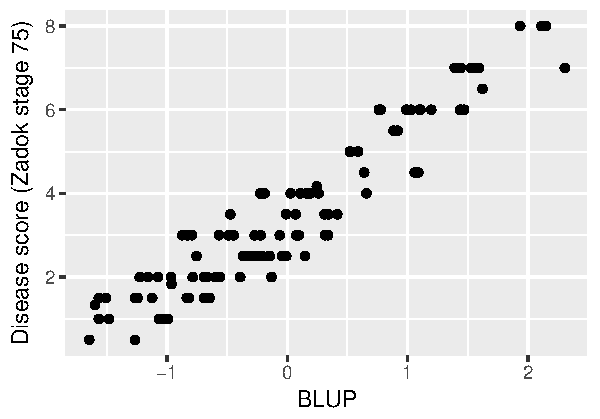
\includegraphics[width=.48\linewidth]{thesis_files/figure-latex/leaf-health-blup-viz-1} }\subfloat[Leaf greenness (Zadok stage 65)\label{fig:leaf-health-blup-viz-2}]{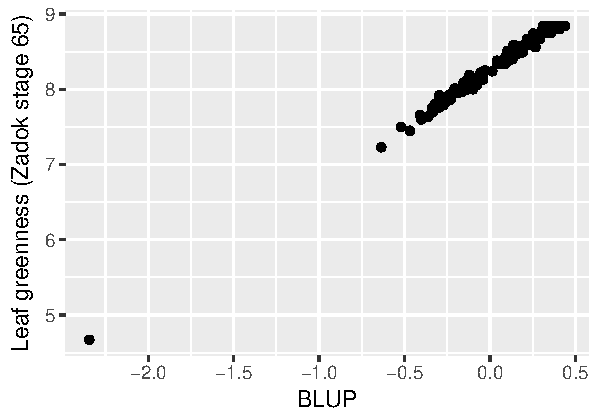
\includegraphics[width=.48\linewidth]{thesis_files/figure-latex/leaf-health-blup-viz-2} }\newline\subfloat[Leaf greenness (Zadok stage 75)\label{fig:leaf-health-blup-viz-3}]{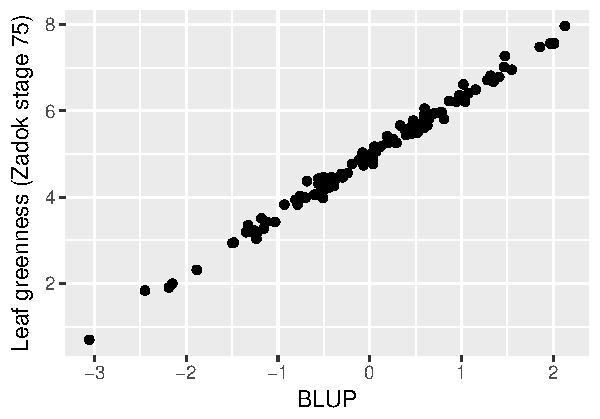
\includegraphics[width=.48\linewidth]{thesis_files/figure-latex/leaf-health-blup-viz-3} }\subfloat[Leaf greenness (Zadok stage 85)\label{fig:leaf-health-blup-viz-4}]{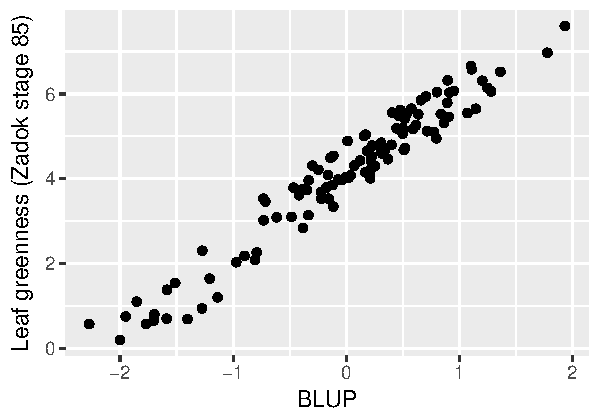
\includegraphics[width=.48\linewidth]{thesis_files/figure-latex/leaf-health-blup-viz-4} }\newline\subfloat[LAUG (Zadok stage 65 to 75)\label{fig:leaf-health-blup-viz-5}]{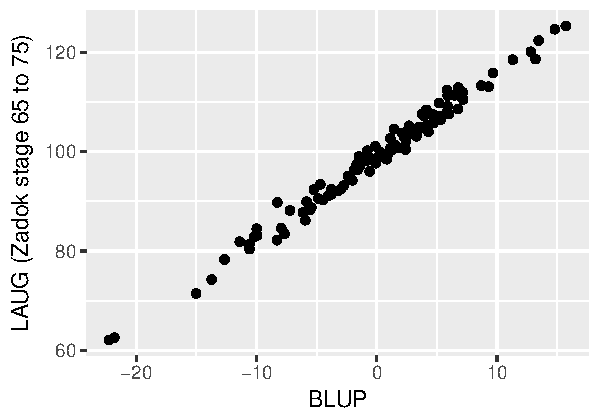
\includegraphics[width=.48\linewidth]{thesis_files/figure-latex/leaf-health-blup-viz-5} }\subfloat[LAUG (Zadok stage 75 to 85)\label{fig:leaf-health-blup-viz-6}]{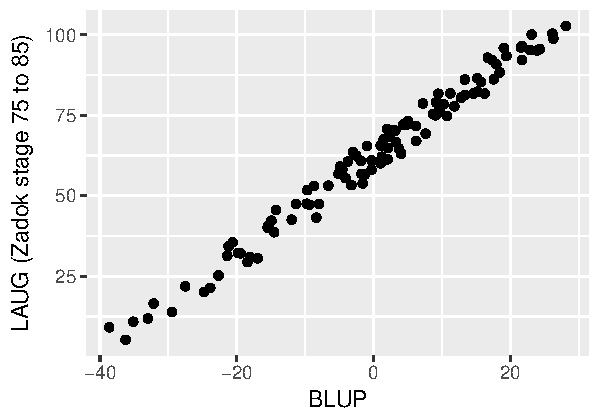
\includegraphics[width=.48\linewidth]{thesis_files/figure-latex/leaf-health-blup-viz-6} }

}

\caption{Scatterplot of observed versus BLUP values of leaf health traits}\label{fig:leaf-health-blup-viz}
\end{figure}
Scatterplot showing observed mean leaf health traits plotted against their respective genotypic BLUP values is presented in Figure \ref{fig:leaf-health-blup-viz}.

The coefficient of determination, as computed by squared correlation coefficient between the observed and fitted values of random effects model are 0.77, 0.73, 0.88, 0.72, 0.75, 0.79, respectively for the Disease score at Zadok's stage 75, Leaf greenness Zadkok's stage 65, Leaf greenness Zadok's stage 75, Leaf greenness Zadok's stage 85, LAUG during Zadok's stage 65 to 75 and LAUG during Zadok's stage 75 to 85.
\begin{figure}[H]

{\centering \subfloat[Disease score (Zadok stage 75)\label{fig:leaf-health-dotplot-1}]{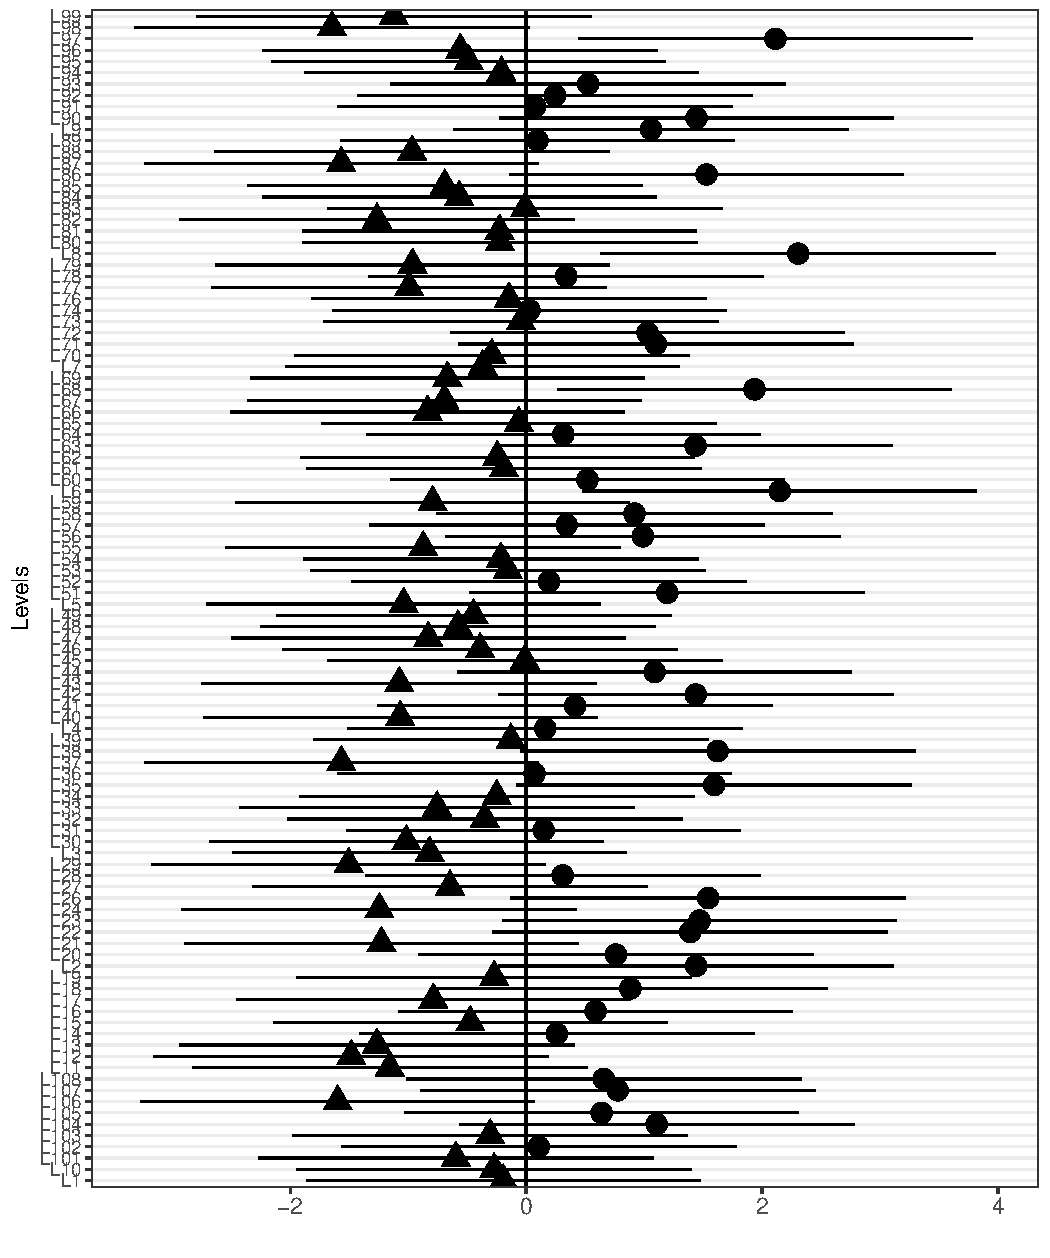
\includegraphics[width=.48\linewidth]{thesis_files/figure-latex/leaf-health-dotplot-1} }\subfloat[Leaf greenness (Zadok stage 65)\label{fig:leaf-health-dotplot-2}]{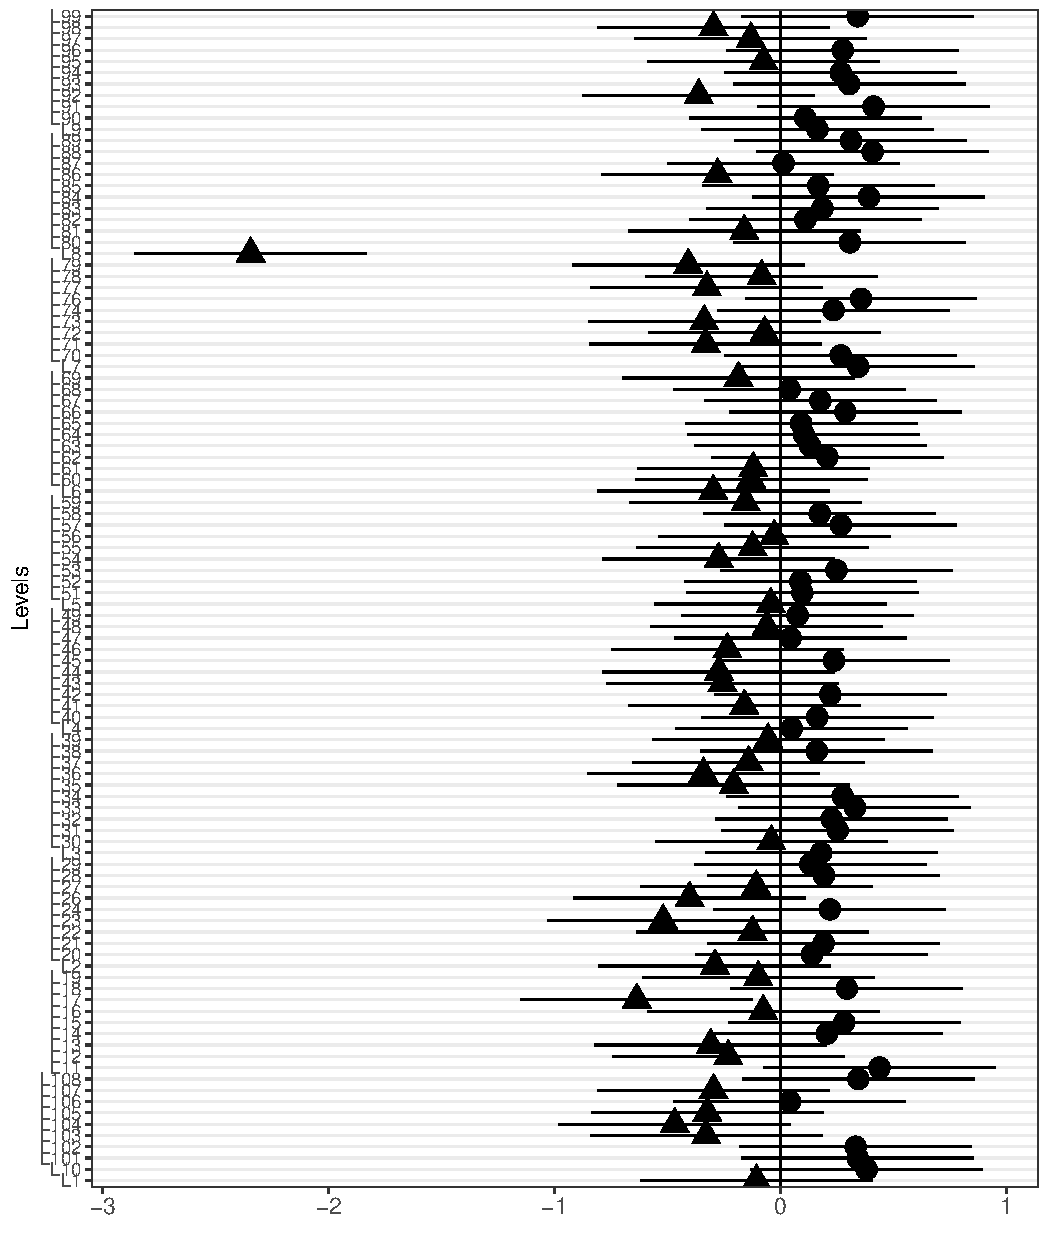
\includegraphics[width=.48\linewidth]{thesis_files/figure-latex/leaf-health-dotplot-2} }\newline\subfloat[Leaf greenness (Zadok stage 75)\label{fig:leaf-health-dotplot-3}]{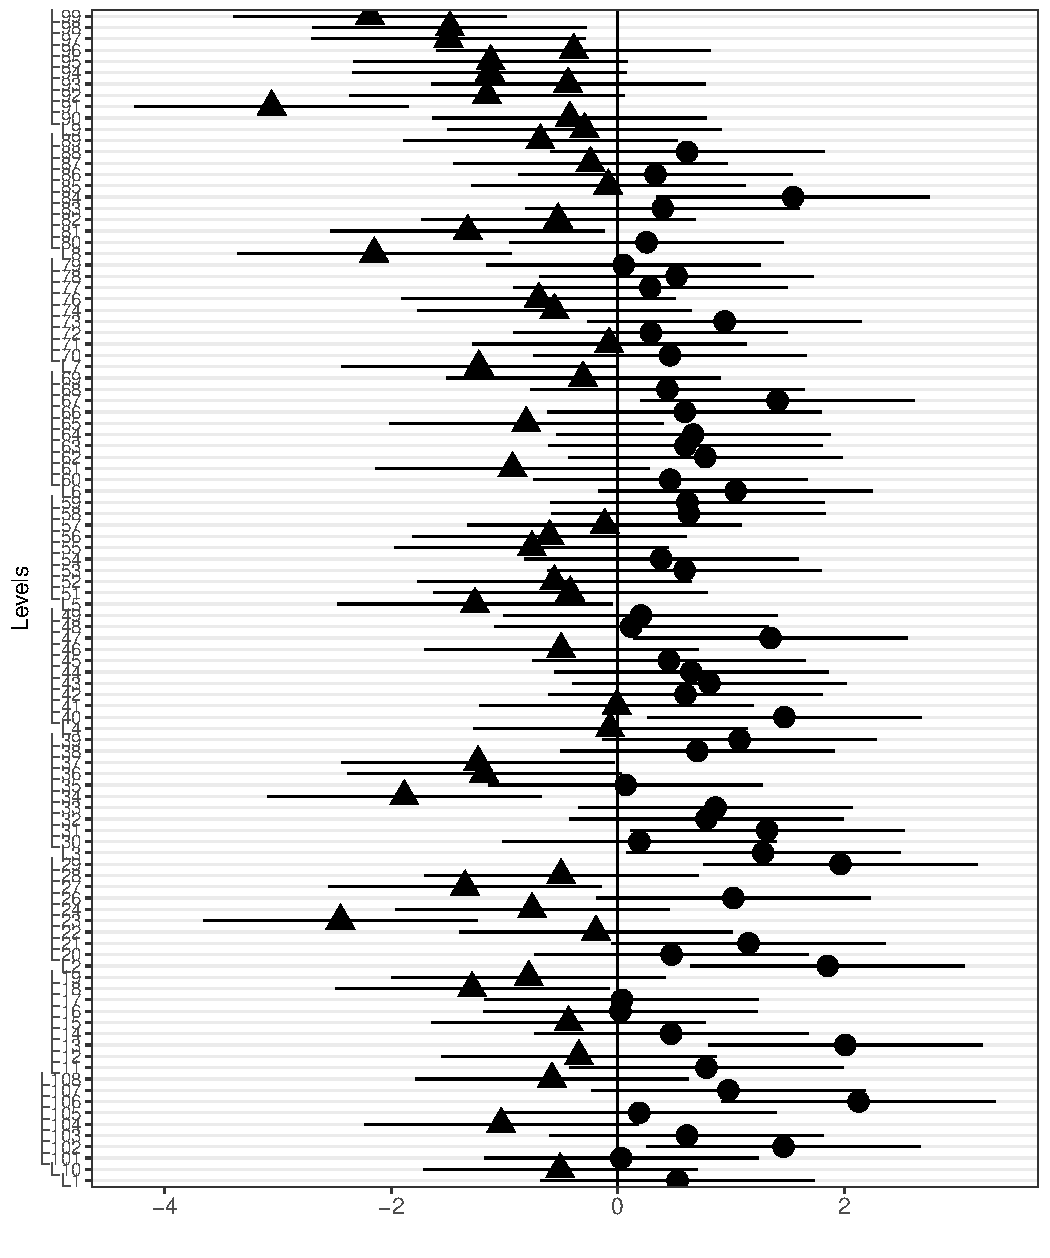
\includegraphics[width=.48\linewidth]{thesis_files/figure-latex/leaf-health-dotplot-3} }\subfloat[Leaf greenness (Zadok stage 85)\label{fig:leaf-health-dotplot-4}]{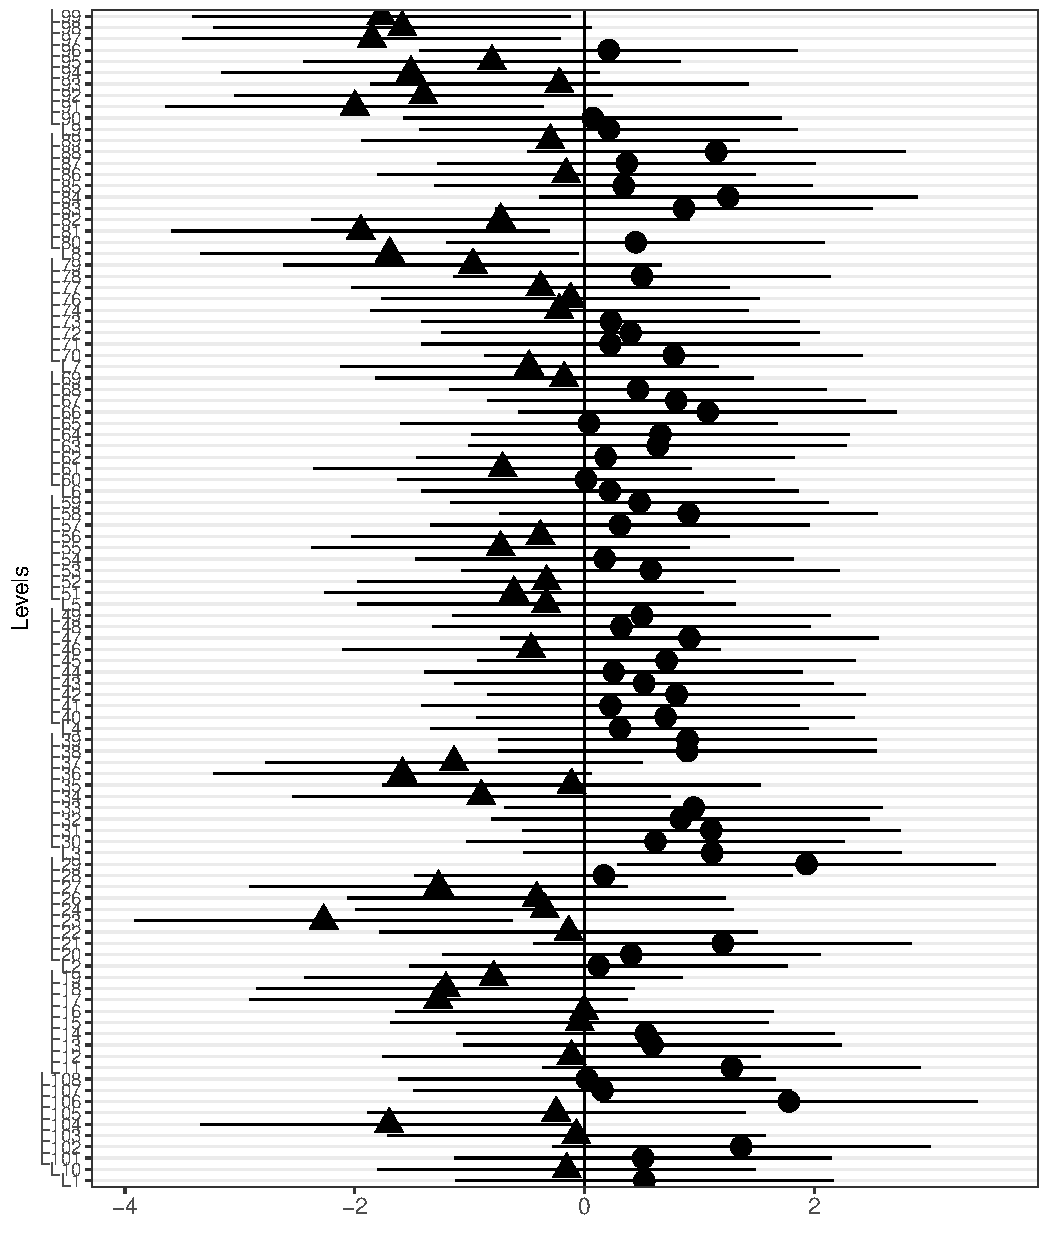
\includegraphics[width=.48\linewidth]{thesis_files/figure-latex/leaf-health-dotplot-4} }

}

\caption{Random effect estimates of leaf health traits of entry genotypes}\label{fig:leaf-health-dotplot}
\end{figure}
\begin{figure}[H]

{\centering \subfloat[LAUG (Zadok stage 65 to 75)\label{fig:leaf-health-dotplot2-1}]{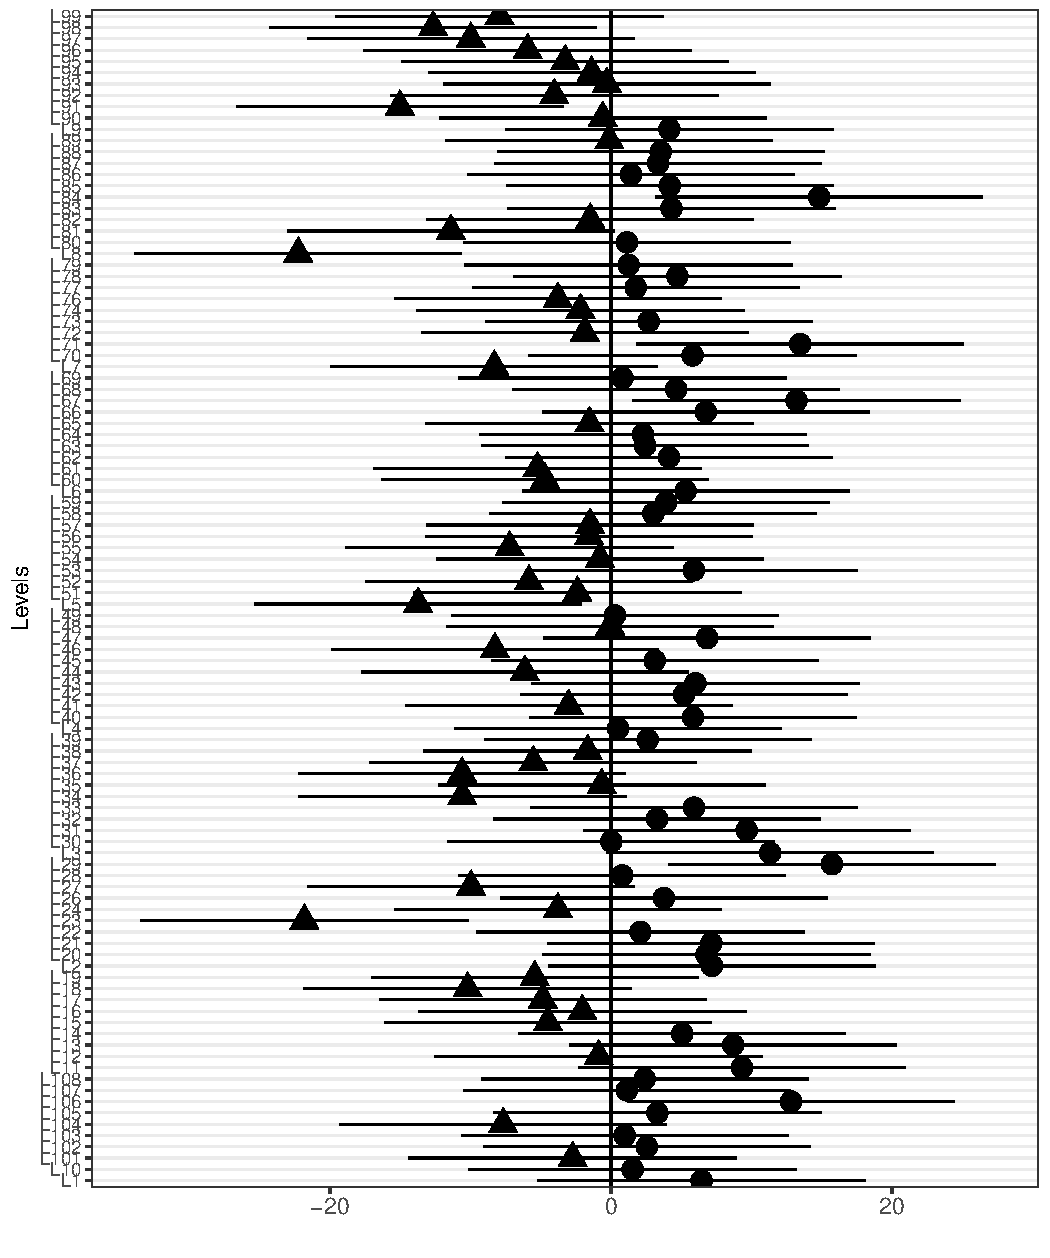
\includegraphics[width=.48\linewidth]{thesis_files/figure-latex/leaf-health-dotplot2-1} }\subfloat[LAUG (Zadok stage 75 to 85)\label{fig:leaf-health-dotplot2-2}]{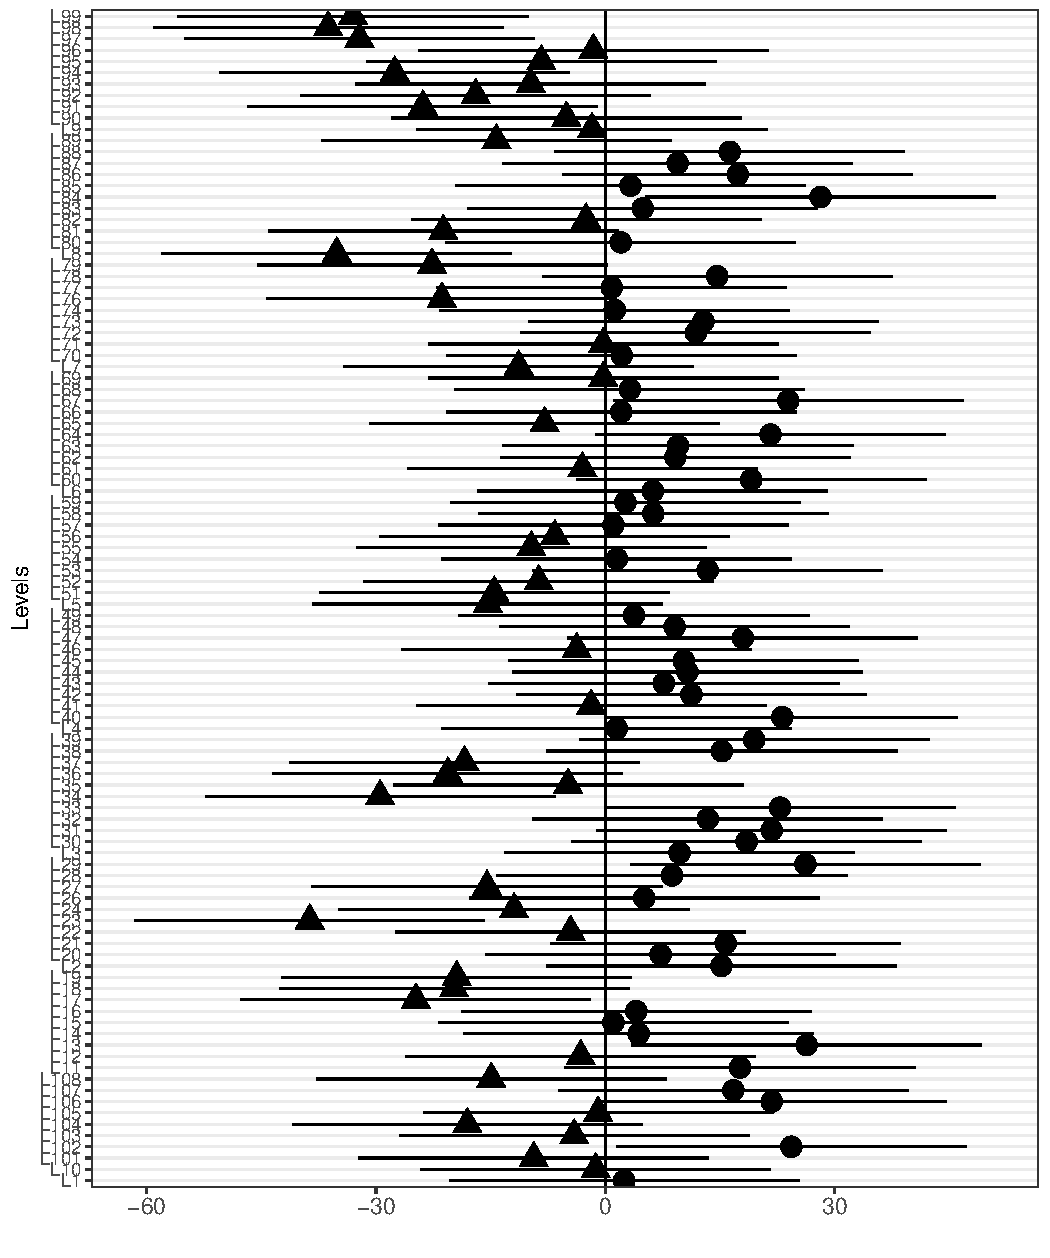
\includegraphics[width=.48\linewidth]{thesis_files/figure-latex/leaf-health-dotplot2-2} }

}

\caption{Random effect estimates of leaf health traits of entry genotypes (...continued)}\label{fig:leaf-health-dotplot2}
\end{figure}
\clearpage

\hypertarget{modeling-plant-morphological-architectural-and-phenological-traits}{%
\section{Modeling plant morphological, architectural and phenological traits}\label{modeling-plant-morphological-architectural-and-phenological-traits}}

\hypertarget{model-estimates-of-plant-morphological-architectural-and-phenological-traits}{%
\subsection{Model estimates of plant morphological, architectural and phenological traits}\label{model-estimates-of-plant-morphological-architectural-and-phenological-traits}}
\begin{landscape}\begingroup\fontsize{8}{10}\selectfont
\begin{longtable}[t]{>{\centering\arraybackslash}p{1.65cm}>{\centering\arraybackslash}p{4.8cm}>{\centering\arraybackslash}p{1.8cm}>{\centering\arraybackslash}p{1.8cm}>{\centering\arraybackslash}p{1.8cm}>{\centering\arraybackslash}p{1.8cm}}
\caption{\label{tab:other-fitted-vs-observed-tab}Model adjusted genotypic mean responses of plant's morphological, architectural and phenological traits}\\
\toprule
encoding & Genotype & Plant height & Leaf area & SPADI & SPADII\\
\midrule
\endfirsthead
\caption[]{\label{tab:other-fitted-vs-observed-tab}Model adjusted genotypic mean responses of plant's morphological, architectural and phenological traits \textit{(continued)}}\\
\toprule
encoding & Genotype & Plant height & Leaf area & SPADI & SPADII\\
\midrule
\endhead
\
\endfoot
\bottomrule
\endlastfoot
1 & Aditya & 103.9 & 37.5 & 46.0 & 38.8\\
2 & Bhrikuti & 94.6 & 38.8 & 44.2 & 35.0\\
3 & Gautam & 105.1 & 41.0 & 44.9 & 38.4\\
4 & Tilottama & 99.2 & 36.0 & 44.5 & 32.3\\
L1 & MUNAL \#1 & 107.5 & 41.5 & 48.3 & 43.8\\
L10 & MUNAL/3/HUW234+LR34/PRINIA//PFAU/WEAVER/4/... & 102.5 & 33.0 & 43.9 & 37.4\\
L101 & PFAU/MILAN/5/CHEN/AEGILOPS SQUARROSA (TAUS)/... & 95.0 & 25.7 & 51.8 & 37.2\\
L102 & PREMIO/5/TUI//2*SUNCO/SA1166/3/TUI/4/FINSI/... & 94.5 & 29.2 & 48.9 & 42.3\\
L103 & PREMIO/BAVIS & 101.0 & 47.0 & 42.2 & 43.0\\
L104 & CHIYAK//ND643/2*WAXWING/3/ND643/2*WAXWING & 94.0 & 25.7 & 43.0 & 21.5\\
L105 & BABAX/LR42//BABAX*2/4/SNI/TRAP\#1/3/KAUZ*2/... & 103.0 & 40.9 & 42.7 & 27.5\\
L106 & PFAU/MILAN//TROST/3/MUNAL \#1/4/PFAU/MILAN//... & 95.3 & 37.6 & 55.0 & 44.6\\
L107 & YUK/AE.SQUARROSA (217)//2*PANDORA & 97.0 & 56.7 & 51.6 & 38.5\\
L108 & SUP152*2//ND643/2*WAXWING & 97.5 & 31.0 & 49.2 & 26.7\\
L11 & SWSR22T.B./5/KAUZ//ALTAR 84/AOS/3/KAUZ/4/... & 93.0 & 26.2 & 42.6 & 37.3\\
L12 & WHEAR/VIVITSI//WHEAR/3/PANDORA & 99.0 & 33.9 & 50.6 & 46.4\\
L13 & WBLL1*2/KURUKU//TACUPETO F2001*2/BRAMBLING & 111.0 & 49.7 & 46.9 & 40.8\\
L14 & PASTOR/3/VORONA/CN079//KAUZ/4/MILAN/OTUS//.. & 102.0 & 43.7 & 40.6 & 40.9\\
L15 & FRANCOLIN \#1*2/ND643/2*WBLL1 & 89.0 & 50.4 & 48.9 & 31.9\\
L16 & KIRITATI/ 2*WBLL1/3/TAM200/PASTOR//TOBA97/4/... & 101.0 & 55.0 & 46.6 & 39.2\\
L17 & SUP152/KENYA SUNBIRD & 99.0 & 40.0 & 45.4 & 44.5\\
L18 & SUP152/KENYA SUNBIRD & 95.0 & 41.5 & 39.8 & 23.3\\
L19 & SUP152/KENYA SUNBIRD & 96.5 & 40.3 & 42.2 & 39.2\\
L2 & KACHU \#1 & 91.0 & 40.1 & 42.4 & 37.4\\
L20 & WBLL1*2/BRAMBLING/5/BABAX/LR42//BABAX*2/4/... & 93.0 & 35.8 & 44.6 & 32.9\\
L21 & ND643/2*WBLL1/3/KIRITATI//2*PRL/2*PASTOR/4/... & 104.0 & 31.9 & 46.6 & 42.9\\
L22 & BETTY/3/CHEN/AE.SQ//2*OPATA/4/BAVIS & 101.5 & 36.5 & 42.1 & 34.4\\
L23 & BAVIS/VORB/5/CROC\_1/AE.SQUARROSA(205)//... & 114.0 & 23.5 & 36.8 & 27.8\\
L24 & BABAX/LR42//BABAX/3/ER2000/4/NAVJ07 & 100.5 & 36.5 & 43.5 & 34.4\\
L26 & NING-MAI-96035/FINSI//HEILO/3/NAVJ07 & 101.0 & 31.0 & 46.5 & 40.3\\
L27 & WBLL1*2/BRAMBLING//TAM200/TUI/3/... & 103.5 & 41.9 & 41.6 & 39.5\\
L28 & KISKADEE \#1/5/KAUZ*2/MNV//KAUZ/3/MILAN/4/... & 92.5 & 56.1 & 44.9 & 39.0\\
L29 & MERCATO//PARUS/PASTOR & 106.5 & 29.1 & 43.9 & 41.4\\
L3 & KACHU/BECARD//WBLL1*2/BRAMBLING & 106.0 & 36.9 & 50.1 & 39.0\\
L30 & PREMIO//PARUS/PASTOR & 95.5 & 51.7 & 51.5 & 43.3\\
L31 & ND643/2*WBLL1//ND643/2*WAXWING & 96.5 & 44.4 & 46.6 & 35.6\\
L32 & ND643/2*WBLL1//ND643/2*WAXWING & 97.0 & 32.9 & 46.6 & 33.9\\
L33 & ND643/2*WBLL1//ND643/2*WAXWING & 95.0 & 32.6 & 47.0 & 41.4\\
L34 & SNB//CMH79A.955/3*CN079/3/ATTILA/4/CHEN/... & 97.5 & 30.3 & 42.3 & 36.9\\
L35 & KIRITATI/ 2*WBLL1/8/SHA7/ PRL/VEE\#6/ 3/ FASAN/... & 106.0 & 39.2 & 38.8 & 32.3\\
L36 & SERI.1B*2/3/KAUZ*2/BOW//KUZ/4/CIRCUS/5/... & 95.5 & 25.5 & 43.0 & 26.3\\
L37 & WHEAR/KUKUNA/3/C80.1/3*BATAVIA//2*WBLL1/4/... & 96.5 & 47.0 & 45.7 & 38.1\\
L38 & BAJ \#1*2/BECARD & 96.5 & 36.5 & 39.9 & 21.0\\
L39 & KACHU*2/MUNAL \#1 & 99.0 & 41.0 & 42.2 & 39.1\\
L4 & PRL/2*PASTOR/3/PFAU/WEAVER*2//CHAPIO & 95.0 & 42.5 & 46.6 & 43.9\\
L40 & KACHU*2/MUNAL \#1 & 97.0 & 36.8 & 45.9 & 45.6\\
L41 & KACHU/2*MUNAL \#1 & 98.0 & 36.8 & 45.0 & 27.0\\
L42 & KACHU/2*MUNAL \#1 & 106.5 & 32.2 & 45.6 & 28.4\\
L43 & KACHU*2/PANDORA & 95.5 & 40.2 & 45.4 & 34.7\\
L44 & SUP152/2*MUNAL \#1 & 100.0 & 35.1 & 45.6 & 24.1\\
L45 & FRNCLN*2/BECARD & 97.0 & 28.4 & 41.7 & 38.3\\
L46 & WBLL1* 2/BRAMBLING//SAAR/2*WAXWING/4/... & 90.0 & 47.9 & 45.4 & 37.1\\
L47 & CHIBIA//PRLII/CM65531/3/MISR 2*2/4/... & 101.0 & 49.2 & 45.5 & 38.7\\
L48 & CHIBIA//PRLII/CM65531/3/MISR 2*2/4/... & 107.5 & 31.1 & 45.9 & 39.9\\
L49 & WAXWING/KRONSTAD F2004//2*FRNCLN & 96.5 & 41.8 & 41.1 & 38.3\\
L5 & DANPHE/CHONTE & 109.5 & 34.9 & 45.0 & 39.4\\
L51 & MUNAL \#1/5/2*PRL/2*PASTOR/4/CHOIX/STAR/3/... & 105.0 & 24.3 & 42.4 & 32.3\\
L52 & MUNAL \#1/5/2*PRL/2*PASTOR/4/CHOIX/STAR/3/... & 102.5 & 24.4 & 42.5 & 36.1\\
L53 & MUNAL \#1/2*FRNCLN & 85.0 & 46.1 & 44.2 & 20.2\\
L54 & MUNAL \#1/2*FRNCLN & 91.5 & 31.4 & 50.0 & 38.3\\
L55 & MUNAL \#1*2//WHEAR/SOKOLL & 94.0 & 38.3 & 42.6 & 29.7\\
L56 & MUNAL \#1*2/KINGBIRD \#1 & 93.0 & 29.1 & 47.4 & 43.5\\
L57 & PRL/2*PASTOR//SUNSTATE/3/MUNAL \#1/4/OTUS//... & 98.5 & 36.4 & 43.5 & 24.9\\
L58 & PRL/2*PASTOR//SUNSTATE/3/MUNAL \#1/4/OTUS//... & 101.0 & 40.8 & 42.2 & 32.4\\
L59 & KAUZ*2/BOW//KAUZ/3/W98.6.38/5/SABUF/4/... & 105.0 & 54.3 & 47.8 & 33.9\\
L6 & SUP152/FRNCLN & 107.0 & 45.5 & 44.0 & 22.7\\
L60 & LERKE/5/KAUZ/3/MYNA/VUL//BUC/FLK/4/MILAN/6/... & 99.0 & 51.3 & 48.8 & 35.9\\
L61 & PASTOR/3/VORONA/CN079//KAUZ/4/MILAN/OTUS//... & 109.5 & 40.0 & 42.0 & 35.1\\
L62 & PASTOR/3/VORONA/CN079//KAUZ/4/MILAN/OTUS//... & 99.5 & 46.8 & 47.0 & 40.5\\
L63 & PFAU/MILAN//TROST/3/PBW65/2*SERI.1B*2/4/... & 97.5 & 35.6 & 45.2 & 39.5\\
L64 & PFAU/MILAN//TROST/3/PBW65/2*SERI.1B*2/4/... & 104.0 & 43.2 & 51.9 & 49.5\\
L65 & DOY1/AE.SQUARROSA (447)/3/KA/NAC//TRCH/4/... & 115.5 & 43.1 & 36.4 & 27.0\\
L66 & MON/IMU//ALD/PVN/3/BORL95/4/OASIS/2*BORL95/... & 103.0 & 51.5 & 49.8 & 39.2\\
L67 & WHEAR/SOKOLL/4/PASTOR//MILAN/KAUZ/3/BAV92 & 101.5 & 40.1 & 47.1 & 38.8\\
L68 & SOKOLL/WBLL1/4/D67.2/PARANA 66.270//... & 98.5 & 46.8 & 41.6 & 28.4\\
L69 & MILAN//PRL/2*PASTOR/4/CROC\_1/AE.SQUARROSA (2... & 99.5 & 38.0 & 45.0 & 33.0\\
L7 & MUU/FRNCLN & 94.5 & 33.4 & 49.4 & 24.3\\
L70 & TRCH/SRTU//KACHU/3/KINGBIRD \#1 & 101.5 & 33.5 & 44.4 & 39.0\\
L71 & TRCH/SRTU//KACHU/3/KINGBIRD \#1 & 97.5 & 32.5 & 43.7 & 33.2\\
L72 & TRCH/5/BAV92//IRENA/KAUZ/3/HUITES/4/DOLL & 104.0 & 36.7 & 44.4 & 39.1\\
L73 & BECARD \#1/3/PBW343*2/KUKUNA//PBW343*2/KUKUNA & 102.5 & 47.2 & 46.5 & 36.3\\
L74 & DANPHE/3/PBW343*2/KUKUNA//PBW343*2/KUKUNA & 112.0 & 30.5 & 50.2 & 37.1\\
L76 & PBW343*2/KUKUNA//PBW343*2/KUKUNA/6/WBLL1*2/... & 107.0 & 32.2 & 47.9 & 40.3\\
L77 & BECARD/6/FRET2*2/4/SNI/TRAP\#1/3/KAUZ*2/TRAP/... & 105.0 & 55.9 & 47.6 & 47.2\\
L78 & KACHU/6/YAR/AE.SQUARROSA (783)/4/GOV/AZ//... & 94.5 & 37.8 & 39.8 & 29.8\\
L79 & FRANCOLIN \#1/NELOKI & 101.0 & 48.7 & 45.7 & 40.4\\
L8 & PRL/ 2*PASTOR/4/CHOIX/STAR/3/HE1/3*CNO79//... & 98.5 & 32.9 & 39.6 & 29.7\\
L80 & PAURAQ/8/NG8201/KAUZ/4/SHA7//PRL/VEE\#6/3/... & 100.5 & 46.2 & 45.5 & 36.2\\
L81 & PRL/2*PASTOR//SUNSTATE/3/GRACK & 104.0 & 39.0 & 38.7 & 34.9\\
L82 & PICAFLOR \#1/NELOKI & 111.5 & 43.5 & 43.6 & 44.2\\
L83 & PICAFLOR \#1/8/NG8201/KAUZ/4/SHA7//PRL/VEE\#6/... & 91.5 & 25.6 & 42.7 & 19.3\\
L84 & NL971*2/MUU & 104.5 & 39.8 & 44.9 & 42.0\\
L85 & MUNAL \#1*2/4/HUW234+LR34/PRINIA//PBW343*2/... & 98.5 & 28.2 & 49.2 & 35.3\\
L86 & MUNAL \#1*2/4/HUW234+LR34/PRINIA//PBW343*2/... & 92.5 & 27.6 & 41.4 & 25.3\\
L87 & MUNAL \#1*2/4/HUW234+LR34/PRINIA//PBW343*2/... & 97.0 & 26.0 & 50.7 & 35.1\\
L88 & MUNAL \#1*2/4/HUW234+LR34/PRINIA//PBW343*2/... & 100.5 & 33.8 & 50.0 & 38.1\\
L89 & BECARD \#1*2/KINGBIRD \#1 & 98.0 & 35.0 & 40.8 & 29.5\\
L9 & DANPHE \#1*2/SHORTENED SR26 TRANSLOCATION & 99.5 & 31.6 & 42.2 & 25.8\\
L90 & BECARD*2/PFUNYE \#1 & 105.0 & 44.7 & 48.1 & 43.2\\
L91 & PBW343/PASTOR//OTUS/TOBA97*2/3/PICAFLOR \#1 & 98.0 & 28.5 & 34.5 & 32.8\\
L92 & ROLF07/KINGBIRD \#1//MUNAL \#1 & 93.0 & 46.4 & 50.7 & 31.2\\
L93 & MUNAL \#1/3/PBW343*2/KUKUNA*2//YANAC & 95.0 & 32.9 & 42.0 & 31.4\\
L94 & SERI.1B*2/3/KAUZ*2/BOW/KAUZ/4/PBW343*2/... & 99.5 & 39.3 & 38.0 & 37.4\\
L95 & KAUZ//ALTAR 84/AOS/3/MILAN/KAUZ/4/SAUAL/5/... & 99.0 & 39.5 & 48.0 & 37.6\\
L96 & PBW343*2/KHVAKI//PARUS/3/PBW343/PASTOR/5/... & 93.0 & 34.0 & 52.0 & 29.0\\
L97 & FRET2*2/4/SNI/TRAP\#1/3/KAUZ*2-TRAP//KAUZ*2/... & 107.0 & 42.5 & 39.0 & 27.0\\
L98 & ATTILA*2/PBW65*2//JUCHI/3/KINGBIRD \#1/4/... & 98.0 & 38.6 & 49.4 & 43.8\\
L99 & MUNAL \#1*2//WBLL1*2/BRAMBLING & 93.5 & 18.7 & 47.5 & 41.1\\*
\end{longtable}
\endgroup{}
\end{landscape}
\clearpage\addtocounter{table}{-1}
\begin{landscape}\begingroup\fontsize{8}{10}\selectfont
\begin{longtable}[t]{>{\centering\arraybackslash}p{1.8cm}>{\centering\arraybackslash}p{5.1cm}>{\centering\arraybackslash}p{2.1cm}>{\centering\arraybackslash}p{2.1cm}>{\centering\arraybackslash}p{2.1cm}}
\caption{\label{tab:other-fitted-vs-observed-tab}Model adjusted genotypic mean responses of plant's morphological, architectural and phenological traits (...continued)}\\
\toprule
encoding & Genotype & CTD & Days to heading & Days to anthesis\\
\midrule
\endfirsthead
\caption[]{\label{tab:other-fitted-vs-observed-tab}Model adjusted genotypic mean responses of plant's morphological, architectural and phenological traits (...continued) \textit{(continued)}}\\
\toprule
encoding & Genotype & CTD & Days to heading & Days to anthesis\\
\midrule
\endhead
\
\endfoot
\bottomrule
\endlastfoot
1 & Aditya & 8.82 & 67.7 & 76.2\\
2 & Bhrikuti & 9.63 & 64.6 & 73.6\\
3 & Gautam & 9.39 & 67.7 & 74.9\\
4 & Tilottama & 9.52 & 62.7 & 71.7\\
L1 & MUNAL \#1 & 11.28 & 74.0 & 85.0\\
L10 & MUNAL/3/HUW234+LR34/PRINIA//PFAU/WEAVER/4/... & 10.71 & 74.0 & 84.0\\
L101 & PFAU/MILAN/5/CHEN/AEGILOPS SQUARROSA (TAUS)/... & 10.59 & 73.0 & 80.0\\
L102 & PREMIO/5/TUI//2*SUNCO/SA1166/3/TUI/4/FINSI/... & 11.77 & 74.0 & 82.0\\
L103 & PREMIO/BAVIS & 11.69 & 75.0 & 84.0\\
L104 & CHIYAK//ND643/2*WAXWING/3/ND643/2*WAXWING & 11.33 & 73.0 & 80.0\\
L105 & BABAX/LR42//BABAX*2/4/SNI/TRAP\#1/3/KAUZ*2/... & 13.68 & 74.0 & 80.0\\
L106 & PFAU/MILAN//TROST/3/MUNAL \#1/4/PFAU/MILAN//... & 2.60 & 74.0 & 82.0\\
L107 & YUK/AE.SQUARROSA (217)//2*PANDORA & 8.54 & 68.0 & 78.0\\
L108 & SUP152*2//ND643/2*WAXWING & 10.37 & 71.0 & 78.0\\
L11 & SWSR22T.B./5/KAUZ//ALTAR 84/AOS/3/KAUZ/4/... & 10.77 & 75.0 & 86.0\\
L12 & WHEAR/VIVITSI//WHEAR/3/PANDORA & 11.30 & 74.0 & 84.0\\
L13 & WBLL1*2/KURUKU//TACUPETO F2001*2/BRAMBLING & 10.69 & 74.0 & 82.0\\
L14 & PASTOR/3/VORONA/CN079//KAUZ/4/MILAN/OTUS//.. & 11.28 & 74.0 & 84.0\\
L15 & FRANCOLIN \#1*2/ND643/2*WBLL1 & 9.03 & 73.0 & 81.0\\
L16 & KIRITATI/ 2*WBLL1/3/TAM200/PASTOR//TOBA97/4/... & 9.83 & 73.0 & 80.0\\
L17 & SUP152/KENYA SUNBIRD & 10.15 & 71.0 & 78.0\\
L18 & SUP152/KENYA SUNBIRD & 11.34 & 63.0 & 73.0\\
L19 & SUP152/KENYA SUNBIRD & 11.72 & 63.0 & 73.0\\
L2 & KACHU \#1 & 9.62 & 71.0 & 80.0\\
L20 & WBLL1*2/BRAMBLING/5/BABAX/LR42//BABAX*2/4/... & 7.95 & 70.0 & 78.0\\
L21 & ND643/2*WBLL1/3/KIRITATI//2*PRL/2*PASTOR/4/... & 10.75 & 74.0 & 80.0\\
L22 & BETTY/3/CHEN/AE.SQ//2*OPATA/4/BAVIS & 9.50 & 70.0 & 78.0\\
L23 & BAVIS/VORB/5/CROC\_1/AE.SQUARROSA(205)//... & 12.89 & 65.0 & 73.0\\
L24 & BABAX/LR42//BABAX/3/ER2000/4/NAVJ07 & 4.80 & 68.0 & 76.0\\
L26 & NING-MAI-96035/FINSI//HEILO/3/NAVJ07 & 9.97 & 68.0 & 78.0\\
L27 & WBLL1*2/BRAMBLING//TAM200/TUI/3/... & 11.53 & 75.0 & 86.0\\
L28 & KISKADEE \#1/5/KAUZ*2/MNV//KAUZ/3/MILAN/4/... & 12.74 & 74.0 & 80.0\\
L29 & MERCATO//PARUS/PASTOR & 11.19 & 74.0 & 85.0\\
L3 & KACHU/BECARD//WBLL1*2/BRAMBLING & 13.35 & 74.0 & 81.0\\
L30 & PREMIO//PARUS/PASTOR & 11.68 & 75.0 & 85.0\\
L31 & ND643/2*WBLL1//ND643/2*WAXWING & 9.71 & 71.0 & 81.0\\
L32 & ND643/2*WBLL1//ND643/2*WAXWING & 10.74 & 73.0 & 80.0\\
L33 & ND643/2*WBLL1//ND643/2*WAXWING & 5.30 & 72.0 & 80.0\\
L34 & SNB//CMH79A.955/3*CN079/3/ATTILA/4/CHEN/... & 8.62 & 75.0 & 85.0\\
L35 & KIRITATI/ 2*WBLL1/8/SHA7/ PRL/VEE\#6/ 3/ FASAN/... & 10.03 & 73.0 & 78.0\\
L36 & SERI.1B*2/3/KAUZ*2/BOW//KUZ/4/CIRCUS/5/... & 11.72 & 72.0 & 78.0\\
L37 & WHEAR/KUKUNA/3/C80.1/3*BATAVIA//2*WBLL1/4/... & 10.25 & 75.0 & 85.0\\
L38 & BAJ \#1*2/BECARD & 10.52 & 70.0 & 78.0\\
L39 & KACHU*2/MUNAL \#1 & 10.05 & 75.0 & 85.0\\
L4 & PRL/2*PASTOR/3/PFAU/WEAVER*2//CHAPIO & 10.75 & 74.0 & 85.0\\
L40 & KACHU*2/MUNAL \#1 & 12.14 & 75.0 & 84.0\\
L41 & KACHU/2*MUNAL \#1 & 10.45 & 65.0 & 73.0\\
L42 & KACHU/2*MUNAL \#1 & 5.30 & 68.0 & 74.0\\
L43 & KACHU*2/PANDORA & 6.42 & 72.0 & 78.0\\
L44 & SUP152/2*MUNAL \#1 & 10.86 & 64.0 & 73.0\\
L45 & FRNCLN*2/BECARD & 10.65 & 75.0 & 84.0\\
L46 & WBLL1* 2/BRAMBLING//SAAR/2*WAXWING/4/... & 11.27 & 75.0 & 86.0\\
L47 & CHIBIA//PRLII/CM65531/3/MISR 2*2/4/... & 8.90 & 73.0 & 82.0\\
L48 & CHIBIA//PRLII/CM65531/3/MISR 2*2/4/... & 11.64 & 73.0 & 84.0\\
L49 & WAXWING/KRONSTAD F2004//2*FRNCLN & 10.96 & 73.0 & 82.0\\
L5 & DANPHE/CHONTE & 11.05 & 75.0 & 85.0\\
L51 & MUNAL \#1/5/2*PRL/2*PASTOR/4/CHOIX/STAR/3/... & 12.11 & 73.0 & 78.0\\
L52 & MUNAL \#1/5/2*PRL/2*PASTOR/4/CHOIX/STAR/3/... & 11.85 & 73.0 & 80.0\\
L53 & MUNAL \#1/2*FRNCLN & 10.22 & 70.0 & 78.0\\
L54 & MUNAL \#1/2*FRNCLN & 9.53 & 75.0 & 85.0\\
L55 & MUNAL \#1*2//WHEAR/SOKOLL & 9.82 & 74.0 & 84.0\\
L56 & MUNAL \#1*2/KINGBIRD \#1 & 10.65 & 73.0 & 80.0\\
L57 & PRL/2*PASTOR//SUNSTATE/3/MUNAL \#1/4/OTUS//... & 6.60 & 71.0 & 78.0\\
L58 & PRL/2*PASTOR//SUNSTATE/3/MUNAL \#1/4/OTUS//... & 4.72 & 72.0 & 78.0\\
L59 & KAUZ*2/BOW//KAUZ/3/W98.6.38/5/SABUF/4/... & 10.70 & 73.0 & 80.0\\
L6 & SUP152/FRNCLN & 9.38 & 70.0 & 78.0\\
L60 & LERKE/5/KAUZ/3/MYNA/VUL//BUC/FLK/4/MILAN/6/... & 8.97 & 75.0 & 85.0\\
L61 & PASTOR/3/VORONA/CN079//KAUZ/4/MILAN/OTUS//... & 9.63 & 74.0 & 80.0\\
L62 & PASTOR/3/VORONA/CN079//KAUZ/4/MILAN/OTUS//... & 11.88 & 74.0 & 84.0\\
L63 & PFAU/MILAN//TROST/3/PBW65/2*SERI.1B*2/4/... & 7.30 & 74.0 & 81.0\\
L64 & PFAU/MILAN//TROST/3/PBW65/2*SERI.1B*2/4/... & 9.88 & 75.0 & 86.0\\
L65 & DOY1/AE.SQUARROSA (447)/3/KA/NAC//TRCH/4/... & 9.00 & 71.0 & 80.0\\
L66 & MON/IMU//ALD/PVN/3/BORL95/4/OASIS/2*BORL95/... & 11.99 & 74.0 & 82.0\\
L67 & WHEAR/SOKOLL/4/PASTOR//MILAN/KAUZ/3/BAV92 & 11.72 & 74.0 & 85.0\\
L68 & SOKOLL/WBLL1/4/D67.2/PARANA 66.270//... & 9.04 & 73.0 & 80.0\\
L69 & MILAN//PRL/2*PASTOR/4/CROC\_1/AE.SQUARROSA (2... & 12.34 & 75.0 & 85.0\\
L7 & MUU/FRNCLN & 10.11 & 72.0 & 78.0\\
L70 & TRCH/SRTU//KACHU/3/KINGBIRD \#1 & 12.15 & 75.0 & 86.0\\
L71 & TRCH/SRTU//KACHU/3/KINGBIRD \#1 & 9.81 & 75.0 & 84.0\\
L72 & TRCH/5/BAV92//IRENA/KAUZ/3/HUITES/4/DOLL & 8.93 & 75.0 & 85.0\\
L73 & BECARD \#1/3/PBW343*2/KUKUNA//PBW343*2/KUKUNA & 8.71 & 73.0 & 82.0\\
L74 & DANPHE/3/PBW343*2/KUKUNA//PBW343*2/KUKUNA & 12.68 & 75.0 & 85.0\\
L76 & PBW343*2/KUKUNA//PBW343*2/KUKUNA/6/WBLL1*2/... & 11.64 & 75.0 & 82.0\\
L77 & BECARD/6/FRET2*2/4/SNI/TRAP\#1/3/KAUZ*2/TRAP/... & 11.53 & 73.0 & 84.0\\
L78 & KACHU/6/YAR/AE.SQUARROSA (783)/4/GOV/AZ//... & 9.69 & 67.0 & 77.0\\
L79 & FRANCOLIN \#1/NELOKI & 5.78 & 70.0 & 78.0\\
L8 & PRL/ 2*PASTOR/4/CHOIX/STAR/3/HE1/3*CNO79//... & 9.72 & 75.0 & 86.0\\
L80 & PAURAQ/8/NG8201/KAUZ/4/SHA7//PRL/VEE\#6/3/... & 6.90 & 75.0 & 85.0\\
L81 & PRL/2*PASTOR//SUNSTATE/3/GRACK & 8.81 & 75.0 & 86.0\\
L82 & PICAFLOR \#1/NELOKI & 12.38 & 75.0 & 86.0\\
L83 & PICAFLOR \#1/8/NG8201/KAUZ/4/SHA7//PRL/VEE\#6/... & 9.82 & 69.0 & 78.0\\
L84 & NL971*2/MUU & 11.45 & 74.0 & 84.0\\
L85 & MUNAL \#1*2/4/HUW234+LR34/PRINIA//PBW343*2/... & 9.76 & 69.0 & 78.0\\
L86 & MUNAL \#1*2/4/HUW234+LR34/PRINIA//PBW343*2/... & 9.93 & 67.0 & 78.0\\
L87 & MUNAL \#1*2/4/HUW234+LR34/PRINIA//PBW343*2/... & 11.75 & 73.0 & 78.0\\
L88 & MUNAL \#1*2/4/HUW234+LR34/PRINIA//PBW343*2/... & 10.22 & 72.0 & 80.0\\
L89 & BECARD \#1*2/KINGBIRD \#1 & 4.55 & 72.0 & 78.0\\
L9 & DANPHE \#1*2/SHORTENED SR26 TRANSLOCATION & 10.55 & 73.0 & 80.0\\
L90 & BECARD*2/PFUNYE \#1 & 11.32 & 73.0 & 82.0\\
L91 & PBW343/PASTOR//OTUS/TOBA97*2/3/PICAFLOR \#1 & 11.70 & 75.0 & 86.0\\
L92 & ROLF07/KINGBIRD \#1//MUNAL \#1 & 6.34 & 74.0 & 80.0\\
L93 & MUNAL \#1/3/PBW343*2/KUKUNA*2//YANAC & 9.73 & 72.0 & 80.0\\
L94 & SERI.1B*2/3/KAUZ*2/BOW/KAUZ/4/PBW343*2/... & 9.47 & 74.0 & 84.0\\
L95 & KAUZ//ALTAR 84/AOS/3/MILAN/KAUZ/4/SAUAL/5/... & 9.62 & 70.0 & 78.0\\
L96 & PBW343*2/KHVAKI//PARUS/3/PBW343/PASTOR/5/... & 8.88 & 74.0 & 84.0\\
L97 & FRET2*2/4/SNI/TRAP\#1/3/KAUZ*2-TRAP//KAUZ*2/... & 10.18 & 74.0 & 82.0\\
L98 & ATTILA*2/PBW65*2//JUCHI/3/KINGBIRD \#1/4/... & 10.50 & 75.0 & 86.0\\
L99 & MUNAL \#1*2//WBLL1*2/BRAMBLING & 11.07 & 75.0 & 86.0\\*
\end{longtable}
\endgroup{}
\end{landscape}
\blandscape

\hypertarget{mixed-model-summary-of-fixed-effects-terms-of-plant-morphological-architectural-and-phenological-traits}{%
\subsection{Mixed model summary of fixed effects terms of plant morphological, architectural and phenological traits}\label{mixed-model-summary-of-fixed-effects-terms-of-plant-morphological-architectural-and-phenological-traits}}

\begingroup 
\footnotesize 
\begin{longtable}{@{\extracolsep{1pt}}lccccc} 
\\[-1.8ex]\hline 
\hline \\[-1.8ex] 
 & \multicolumn{5}{c}{\textit{Dependent variable:}} \\ 
\cline{2-6} 
\\[-1.8ex] & \multicolumn{5}{c}{\textit{linear}} \\ 
 & \multicolumn{5}{c}{\textit{mixed-effects}} \\ 
 & \parbox[t]{2.5cm}{Plant height} & \parbox[t]{2.5cm}{Leaf area} & \parbox[t]{2.5cm}{SPAD I} & \parbox[t]{2.5cm}{SPAD II} & \parbox[t]{2.5cm}{Canopy temperature depression (CTD)} \\ 
\\[-1.8ex] & (1) & (2) & (3) & (4) & (5)\\ 
\hline \\[-1.8ex] 
 Bhrikuti & $-$9.46$^{***}$ (1.17) & 1.51 (1.79) & $-$1.74$^{***}$ (0.60) & $-$3.78$^{**}$ (1.61) & 0.52$^{**}$ (0.24) \\ 
  & p = 0.00 & p = 0.40 & p = 0.004 & p = 0.02 & p = 0.04 \\ 
  Gautam & 1.21 (1.17) & 3.28$^{*}$ (1.81) & $-$1.06$^{*}$ (0.61) & $-$0.38 (1.62) & 0.20 (0.24) \\ 
  & p = 0.31 & p = 0.07 & p = 0.08 & p = 0.82 & p = 0.42 \\ 
  Tilottama & $-$4.92$^{***}$ (1.17) & $-$1.49 (1.80) & $-$1.38$^{**}$ (0.61) & $-$6.46$^{***}$ (1.62) & 0.43$^{*}$ (0.24) \\ 
  & p = 0.0001 & p = 0.41 & p = 0.03 & p = 0.0001 & p = 0.08 \\ 
  Aditaya (Constant) & 104.00$^{***}$ (2.23) & 37.60$^{***}$ (2.39) & 45.90$^{***}$ (2.73) & 38.80$^{***}$ (1.37) & 9.07$^{***}$ (0.79) \\ 
  & p = 0.00 & p = 0.00 & p = 0.00 & p = 0.00 & p = 0.00 \\ 
 \hline \\[-1.8ex] 
Observations & 238 & 238 & 238 & 238 & 238 \\ 
Log Likelihood & $-$730.00 & $-$821.00 & $-$600.00 & $-$782.00 & $-$378.00 \\ 
Akaike Inf. Crit. & 1,484.00 & 1,666.00 & 1,224.00 & 1,587.00 & 780.00 \\ 
Bayesian Inf. Crit. & 1,525.00 & 1,707.00 & 1,265.00 & 1,629.00 & 821.00 \\ 
\hline 
\hline \\[-1.8ex] 
\textit{Note:}  & \multicolumn{5}{r}{$^{*}$p$<$0.1; $^{**}$p$<$0.05; $^{***}$p$<$0.01} \\ 
\end{longtable} 
\endgroup

\begingroup 
\small 
\begin{longtable}{@{\extracolsep{1pt}}lcc} 
\\[-1.8ex]\hline 
\hline \\[-1.8ex] 
 & \multicolumn{2}{c}{\textit{Dependent variable:}} \\ 
\cline{2-3} 
\\[-1.8ex] & \multicolumn{2}{c}{\textit{linear}} \\ 
 & \multicolumn{2}{c}{\textit{mixed-effects}} \\ 
 & \parbox[t]{2.5cm}{Days to heading} & \parbox[t]{2.5cm}{Days to anthesis} \\ 
\\[-1.8ex] & (1) & (2)\\ 
\hline \\[-1.8ex] 
 Bhrikuti & $-$3.22$^{***}$ (0.37) & $-$2.75$^{***}$ (0.45) \\ 
  & p = 0.00 & p = 0.00 \\ 
  Gautam & $-$0.19 (0.38) & $-$1.59$^{***}$ (0.46) \\ 
  & p = 0.62 & p = 0.001 \\ 
  Tilottama & $-$5.07$^{***}$ (0.38) & $-$4.65$^{***}$ (0.46) \\ 
  & p = 0.00 & p = 0.00 \\ 
  Aditaya (Constant) & 67.80$^{***}$ (2.40) & 76.30$^{***}$ (3.10) \\ 
  & p = 0.00 & p = 0.00 \\ 
 \hline \\[-1.8ex] 
Observations & 238 & 238 \\ 
Log Likelihood & $-$509.00 & $-$560.00 \\ 
Akaike Inf. Crit. & 1,042.00 & 1,145.00 \\ 
Bayesian Inf. Crit. & 1,084.00 & 1,186.00 \\ 
\hline 
\hline \\[-1.8ex] 
\textit{Note:}  & \multicolumn{2}{r}{$^{*}$p$<$0.1; $^{**}$p$<$0.05; $^{***}$p$<$0.01} \\ 
\end{longtable} 
\endgroup

\elandscape

\hypertarget{plant-height}{%
\subsubsection{Plant height}\label{plant-height}}

Highly significant difference exist among the genotypes for Plant height trait based on the significane of LRT using \(\chi^2\) statistic (\(59.5\) with \(4\ df\)).

A pairwise contrast of fixed effects estimate shows that all check varieties differ from one another except for Aditya (mean: \(103.00\ cm\ (\pm\ 1.4)\)) and Gautam (which are similar at 0.05 level of significance), implying that plant height is an important trait to differentiate the genotypes (indicated by a p-value of less than 0.01). With an average height of \(94.53\ cm\ (\pm\ 1.4)\), Bhrikuti is the shortest variety. Likewise, the tallest variety (Gautam) has the mean height of \(102.86\ cm\ (\pm\ 1.41)\).

Meanwhile, random effects estimates for entry genotype levels do not show as much of difference. Also, the non-significance of LRT comparing models with and without random terms for entry genotypes clearly indicates that no relationship exists between plant height and entry genotypes. ANOVA table (\ref{tab:lrt-plht}) and the dotplot (Figure \ref{fig:other-dotplot11}) showing random effects estimates of the entry genotypes illustrate the relationship.

However, blocking factors -- row nested within rowgroup and superimposed blocks arising from the intersection between rowgroup and colgroup -- have contributed significantly to the variation in plant height.
\begin{table}[H]

\caption{\label{tab:other-meanconf-tab1}Mean differences in Plant height of check varieties (post-hoc comparison using Tukey procedure)}
\centering
\begin{tabular}[t]{cccccccc}
\toprule
Contrast & Estimate & Std. Error & df & t value & lower & upper & Pr(>|t|)\\
\midrule
Aditya-Bhrikuti & 9.46 & 1.17 & 106 & 8.10 & 7.14 & 11.77 & 0.000\\
Aditya-Gautam & -1.21 & 1.18 & 106 & -1.03 & -3.54 & 1.12 & 0.305\\
Aditya-Tilottama & 4.92 & 1.17 & 105 & 4.19 & 2.59 & 7.24 & 0.000\\
Bhrikuti-Gautam & -10.67 & 1.17 & 106 & -9.08 & -13.00 & -8.34 & 0.000\\
Bhrikuti-Tilottama & -4.54 & 1.17 & 105 & -3.87 & -6.87 & -2.22 & 0.000\\
Gautam-Tilottama & 6.13 & 1.18 & 106 & 5.18 & 3.78 & 8.47 & 0.000\\
\bottomrule
\end{tabular}
\end{table}
\hypertarget{flag-leaf-surface-area}{%
\subsubsection{Flag leaf surface area}\label{flag-leaf-surface-area}}

No significant difference exist among the genotypes for Flag leaf surface area trait based on the non significance of LRT using \(\chi^2\) statistic (ANOVA Table \ref{tab:lrt-lar}).

A pairwise contrast of fixed effects estimate however reveals that check varieties Gautam (mean: \(41.0\ cm^2\ (\pm\ 1.81)\)) and Tilottama (mean: \(36.0\ cm^2\ (\pm\ 1.80)\)) had different flag leaf surface area, indicated by a p-value of less than 0.05.

However, effect of blocking factor -- row nested within rowgroup -- can be confirmed as signifcant source of environmental variability in the flag leaf area trait (based on LRT).
\begin{table}[H]

\caption{\label{tab:other-meanconf-tab2}Mean differences in Flag leaf area of check varieties (post-hoc comparison using Tukey procedure)}
\centering
\begin{tabular}[t]{cccccccc}
\toprule
Contrast & Estimate & Std. Error & df & t value & lower & upper & Pr(>|t|)\\
\midrule
Aditya-Bhrikuti & -1.51 & 1.79 & 110 & -0.844 & -5.070 & 2.041 & 0.400\\
Aditya-Gautam & -3.28 & 1.81 & 110 & -1.816 & -6.864 & 0.299 & 0.072\\
Aditya-Tilottama & 1.49 & 1.80 & 110 & 0.825 & -2.087 & 5.066 & 0.411\\
Bhrikuti-Gautam & -1.77 & 1.80 & 109 & -0.981 & -5.340 & 1.803 & 0.329\\
Bhrikuti-Tilottama & 3.00 & 1.80 & 109 & 1.667 & -0.567 & 6.576 & 0.098\\
Gautam-Tilottama & 4.77 & 1.82 & 110 & 2.627 & 1.172 & 8.374 & 0.010\\
\bottomrule
\end{tabular}
\end{table}
\hypertarget{spad-at-zadoks-stage-65}{%
\subsubsection{SPAD at Zadok's stage 65}\label{spad-at-zadoks-stage-65}}

No significant difference exist among the genotypes SPAD measurement at Zadok's stage 65 based on the non significance of LRT using \(\chi^2\) statistic. However, the test statistic of 8.95 at 4 df indicates that the hypotheis of no-difference do not hold at \(10\%\) level of significance.

A pairwise contrast of fixed effects estimate, however, reveals that check variety Aditya has a higher mean SPAD value (\(45.90\ (\pm\ 2.73)\)) than both check varieties Bhrikuti and Tilottama. The variety with the lowest relative chlorophyll content at the given stage is Bhrikuti (\(44.20\ (\pm\ 2.73)\)).

Likewise, highly variable estimates of random effects (Shown in \ref{fig:other-dotplot13}) along with significance of LRT (Shown in \ref{tab:lrt-spadi}) indicates that the entry genotypes vary to a large extent in the leaf chlorophyll content, early in the reproductive phase of the crop.

Meanwhile, blocking factors do not have significant effects associated with the trait at the reference level of significance (\(\alpha=0.05\)).
\begin{table}[H]

\caption{\label{tab:other-meanconf-tab3}Mean differences in SPADI (Zadok's stage 65) of check varieties (post-hoc comparison using Tukey procedure)}
\centering
\begin{tabular}[t]{cccccccc}
\toprule
Contrast & Estimate & Std. Error & df & t value & lower & upper & Pr(>|t|)\\
\midrule
Aditya-Bhrikuti & 1.739 & 0.603 & 107 & 2.884 & 0.544 & 2.935 & 0.005\\
Aditya-Gautam & 1.064 & 0.608 & 105 & 1.752 & -0.140 & 2.269 & 0.083\\
Aditya-Tilottama & 1.380 & 0.607 & 104 & 2.273 & 0.176 & 2.584 & 0.025\\
Bhrikuti-Gautam & -0.675 & 0.607 & 106 & -1.113 & -1.878 & 0.528 & 0.268\\
Bhrikuti-Tilottama & -0.359 & 0.606 & 105 & -0.592 & -1.561 & 0.843 & 0.555\\
Gautam-Tilottama & 0.316 & 0.611 & 105 & 0.517 & -0.896 & 1.528 & 0.606\\
\bottomrule
\end{tabular}
\end{table}
\hypertarget{spad-at-zadoks-stage-85}{%
\subsubsection{SPAD at Zadok's stage 85}\label{spad-at-zadoks-stage-85}}

LRT of mixed models using \(\chi^2\) statistic show that highly significant differences exist among the genotypes for the SPAD measured at Zadok's stage 85.

A pairwise contrast of fixed effects estimate, however, reveals that check variety Aditya (\(38.80\ (\pm\ 1.37)\)) has the higher mean SPAD values in comparison to check varieties Bhrikuti and Tilottama, although no significant difference exist between the most chlorophyll preserved variety (Aditya) and the Gautam. Similarly, the mean comparison also shows that check variety Gautam also has higher relative chlorophyll content than other two check varieties. The lowest mean SPAD values was recorded for Tilottama (\(32.35\ (\pm\ 1.37)\)) the given stage.

In contrast, the entry genotypes do not present as much a variation as check cultivars do among each other for SPAD measurement at latter stage of growth. This is evident from LRT test shown in \ref{tab:lrt-spadii} and also random effects estimate of the entry genotypes (Shown in \ref{fig:other-dotplot14}). Similarly, blocking factors do not present an attributable source of variation for the trait.
\begin{table}[H]

\caption{\label{tab:other-meanconf-tab4}Mean differences in SPADII (Zadok's stage 85) of check varieties (post-hoc comparison using Tukey procedure)}
\centering
\begin{tabular}[t]{cccccccc}
\toprule
Contrast & Estimate & Std. Error & df & t value & lower & upper & Pr(>|t|)\\
\midrule
Aditya-Bhrikuti & 3.78 & 1.61 & 126 & 2.352 & 0.599 & 6.962 & 0.020\\
Aditya-Gautam & 0.38 & 1.62 & 126 & 0.235 & -2.826 & 3.585 & 0.815\\
Aditya-Tilottama & 6.46 & 1.62 & 126 & 3.990 & 3.258 & 9.668 & 0.000\\
Bhrikuti-Gautam & -3.40 & 1.62 & 126 & -2.100 & -6.605 & -0.196 & 0.038\\
Bhrikuti-Tilottama & 2.68 & 1.62 & 126 & 1.657 & -0.522 & 5.887 & 0.100\\
Gautam-Tilottama & 6.08 & 1.63 & 126 & 3.729 & 2.854 & 9.311 & 0.000\\
\bottomrule
\end{tabular}
\end{table}
\hypertarget{canopy-temperature-depression-ctd}{%
\subsubsection{Canopy temperature depression (CTD)}\label{canopy-temperature-depression-ctd}}

LRT of mixed models using \(\chi^2\) statistic show that genotypes have significant differences for the crop architecture trait Canopy temperature depression (CTD) measured near anthesis stage.

Pairwise comparison, using Tukey procedure, of fixed effects estimate shows that canopy structure of check variety Bhrikuti favors greater reduction in temperature than check variety Aditya (\(9.08^\circ C\ (\pm\ 0.79)\)). Other varieties were at par with both of the check varieties. The

In contrast, the entry genotypes do not present attributable variation in CTD. This is evident from LRT test shown in \ref{tab:lrt-ctd} and also the variance components decomposition of random effects terms, which shows no heritable variation is found among the tested entries.

Although, multiple blocking factors, comprising effects of row group, nested effects of columns within column group and the effects of superimposed blocks arising from the intersection of individual row group and column group are found significantly high for the variation in canopy temperature depression trait.
\begin{table}[H]

\caption{\label{tab:other-meanconf-tab5}Mean differences in CTD of check varieties (post-hoc comparison using Tukey procedure)}
\centering
\begin{tabular}[t]{cccccccc}
\toprule
Contrast & Estimate & Std. Error & df & t value & lower & upper & Pr(>|t|)\\
\midrule
Aditya-Bhrikuti & -0.519 & 0.243 & 206 & -2.139 & -0.998 & -0.041 & 0.034\\
Aditya-Gautam & -0.199 & 0.244 & 206 & -0.815 & -0.681 & 0.283 & 0.416\\
Aditya-Tilottama & -0.433 & 0.244 & 207 & -1.773 & -0.915 & 0.048 & 0.078\\
Bhrikuti-Gautam & 0.320 & 0.245 & 207 & 1.306 & -0.163 & 0.803 & 0.193\\
Bhrikuti-Tilottama & 0.086 & 0.244 & 206 & 0.352 & -0.396 & 0.568 & 0.725\\
Gautam-Tilottama & -0.234 & 0.246 & 207 & -0.950 & -0.720 & 0.252 & 0.343\\
\bottomrule
\end{tabular}
\end{table}
\hypertarget{days-to-heading}{%
\subsubsection{Days to heading}\label{days-to-heading}}

Highly significant difference exists among the genotypes for days to heading trait based on the significane of LRT using \(\chi^2\) statistic (155 with 4 degrees of freedom).

Pairwise comparison of fixed effects estimate shows that all check varieties differ from one another except for Aditya (late heading type) (with mean of \(67.79\ (\pm\ 2.40)\) days) and Gautam, which require similar Days for heading. Mean number of days taken for head to develop in half of the population was lowest in Tilottama (\(62.71\ (\pm\ 2.40)\) days) variety.

Similarly, random effects estimates for entry genotype levels also exhibit high variation for the trait, thereby indicating that significant proportion of the variation is heritable. ANOVA table (\ref{tab:lrt-dth}) and the dotplot (Figure \ref{fig:other-dotplot22}) showing random effects estimates of the entry genotypes illustrate the relationship. Amongst blocking factors, the effect of grouping the experimental units in rowgroups has relevance in reducing extraneous source of variability carried to the trait in the field.
\begin{table}[H]

\caption{\label{tab:other-meanconf-tab6}Mean differences in Days to heading of check varieties (post-hoc comparison using Tukey procedure)}
\centering
\begin{tabular}[t]{cccccccc}
\toprule
Contrast & Estimate & Std. Error & df & t value & lower & upper & Pr(>|t|)\\
\midrule
Aditya-Bhrikuti & 3.221 & 0.373 & 113 & 8.635 & 2.482 & 3.960 & 0.000\\
Aditya-Gautam & 0.187 & 0.376 & 111 & 0.496 & -0.558 & 0.931 & 0.621\\
Aditya-Tilottama & 5.073 & 0.375 & 111 & 13.511 & 4.329 & 5.817 & 0.000\\
Bhrikuti-Gautam & -3.034 & 0.376 & 113 & -8.077 & -3.779 & -2.290 & 0.000\\
Bhrikuti-Tilottama & 1.852 & 0.375 & 112 & 4.934 & 1.108 & 2.596 & 0.000\\
Gautam-Tilottama & 4.887 & 0.379 & 112 & 12.909 & 4.137 & 5.637 & 0.000\\
\bottomrule
\end{tabular}
\end{table}
\hypertarget{days-to-anthesis}{%
\subsubsection{Days to anthesis}\label{days-to-anthesis}}

Highly significant difference exists among the genotypes for Number of days to anthesis trait based on the significane of LRT using \(\chi^2\) statistic (\(85.8\) with \(4\ df\)).

Pairwise comparison of fixed effects estimate shows that all check varieties differ from one another, with longest period to anthesis being that of check variety Aditya (\(76.30\ (\pm\ 3.10)\) days) and the earliest flowering cultivar being Tilottama with an average of \(71.7\ (\pm\ 0.46)\) days.

Similarly, entry genotype also have a considerable genotypic variation which is reflected in a large measure of variance in random effects term. ANOVA table (\ref{tab:lrt-dta}) and the dotplot (Figure \ref{fig:other-dotplot23}) showing random effects estimates of the entry genotypes illustrate the relationship. Likewise, the effects of rowgroup and colgroup, contributing significantly to the variation in trait, may be safely substracted for obtaining better effects estimates of the entry genotypes.
\begin{figure}[H]

{\centering 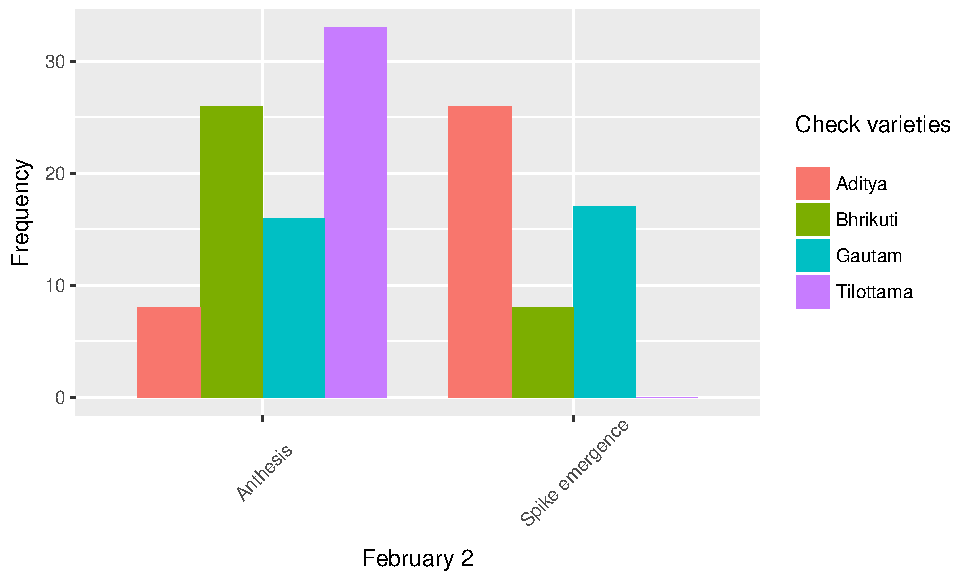
\includegraphics[width=0.80\linewidth]{thesis_files/figure-latex/cor-graph-barplot-viz-checks-1} 

}

\caption{Number of checks at different growth stages at February 2}\label{fig:cor-graph-barplot-viz-checks}
\end{figure}
Frequency barplot of different stages of reproductive periods of growth in wheat (Figure \ref{fig:cor-graph-barplot-viz-checks}) reaffirms that Tilottama variety flowers the earliest amongst the check varieties and Aditya reaches to the flowering relatively late.
\begin{table}[H]

\caption{\label{tab:other-meanconf-tab7}Mean differences in Days to anthesis of check varieties (post-hoc comparison using Tukey procedure)}
\centering
\begin{tabular}[t]{cccccccc}
\toprule
Contrast & Estimate & Std. Error & df & t value & lower & upper & Pr(>|t|)\\
\midrule
Aditya-Bhrikuti & 2.75 & 0.453 & 105 & 6.07 & 1.854 & 3.65 & 0.000\\
Aditya-Gautam & 1.59 & 0.457 & 105 & 3.48 & 0.683 & 2.50 & 0.001\\
Aditya-Tilottama & 4.65 & 0.456 & 105 & 10.19 & 3.747 & 5.56 & 0.000\\
Bhrikuti-Gautam & -1.16 & 0.456 & 104 & -2.55 & -2.067 & -0.26 & 0.012\\
Bhrikuti-Tilottama & 1.90 & 0.456 & 104 & 4.17 & 0.996 & 2.80 & 0.000\\
Gautam-Tilottama & 3.06 & 0.460 & 104 & 6.66 & 2.151 & 3.97 & 0.000\\
\bottomrule
\end{tabular}
\end{table}
\hypertarget{mean-comparison-of-plants-morphological-architectural-and-phenological-traits-of-entry-genotypes}{%
\subsection{Mean comparison of plant's morphological, architectural and phenological traits of entry genotypes}\label{mean-comparison-of-plants-morphological-architectural-and-phenological-traits-of-entry-genotypes}}
\begin{figure}[H]

{\centering \subfloat[Plant height\label{fig:other-blup-viz-1}]{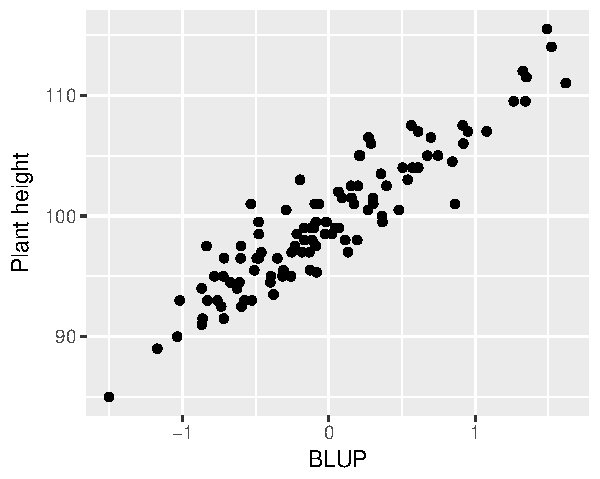
\includegraphics[width=.48\linewidth]{thesis_files/figure-latex/other-blup-viz-1} }\subfloat[Flag leaf area\label{fig:other-blup-viz-2}]{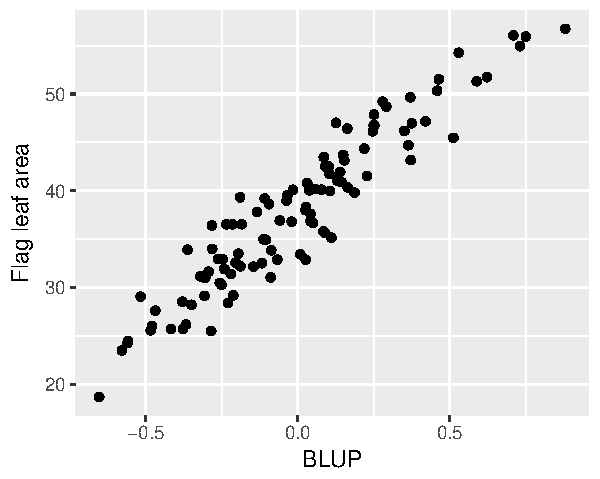
\includegraphics[width=.48\linewidth]{thesis_files/figure-latex/other-blup-viz-2} }\newline\subfloat[SPADI (Zadok's stage 65)\label{fig:other-blup-viz-3}]{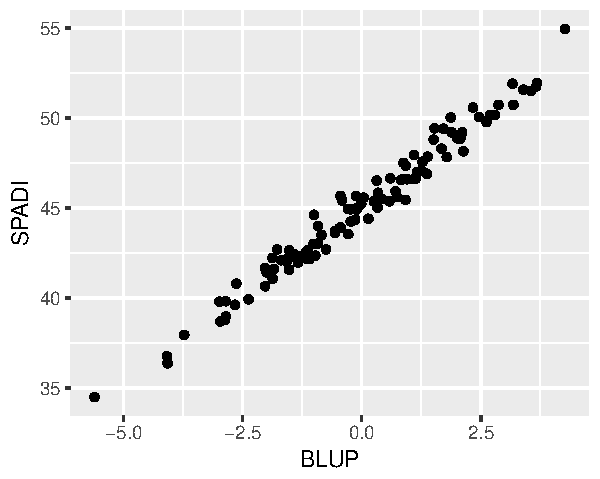
\includegraphics[width=.48\linewidth]{thesis_files/figure-latex/other-blup-viz-3} }\subfloat[SPADII (Zadok's stage 85)\label{fig:other-blup-viz-4}]{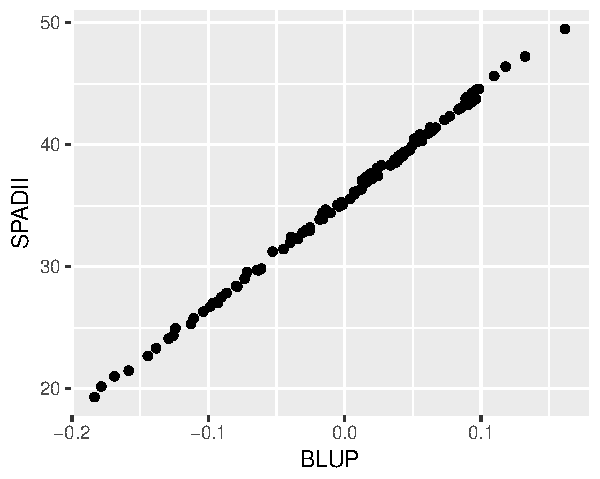
\includegraphics[width=.48\linewidth]{thesis_files/figure-latex/other-blup-viz-4} }

}

\caption{Scatterplot of observed versus BLUP values of plant morphological, architectural and phenological traits}\label{fig:other-blup-viz}
\end{figure}
Scatterplot showing observed means of plant's morphological, phenological and architectural traits plotted against their respective genotypic BLUP values is presented in Figure \ref{fig:other-blup-viz}.

The coefficient of determination, as computed by squared correlation coefficient between the observed and fitted values of random effects model are 0.56, 0.33, 0.7, 0.1, 0.81, 0.92, 0.91, respectively for the Plant height, Flag leaf area, SPAD at Zadok's stage 65, SPAD at Zadok's stage 85, Canopy temperature depression, Days to heading and Days to anthesis.
\begin{figure}[H]

{\centering \subfloat[Canopy temperature depression (CTD)\label{fig:other-blup-viz2-1}]{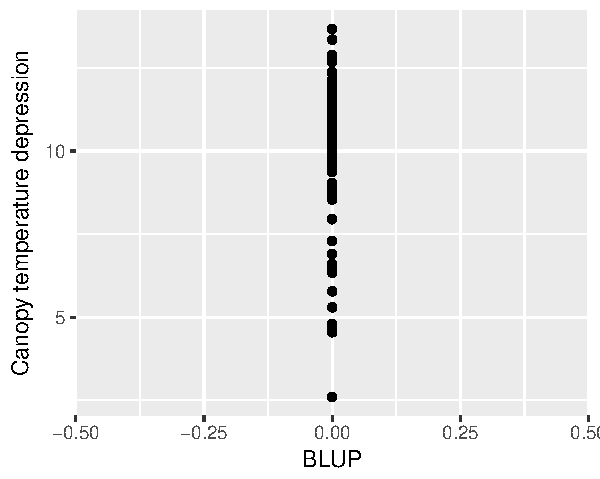
\includegraphics[width=.48\linewidth]{thesis_files/figure-latex/other-blup-viz2-1} }\subfloat[Days to heading\label{fig:other-blup-viz2-2}]{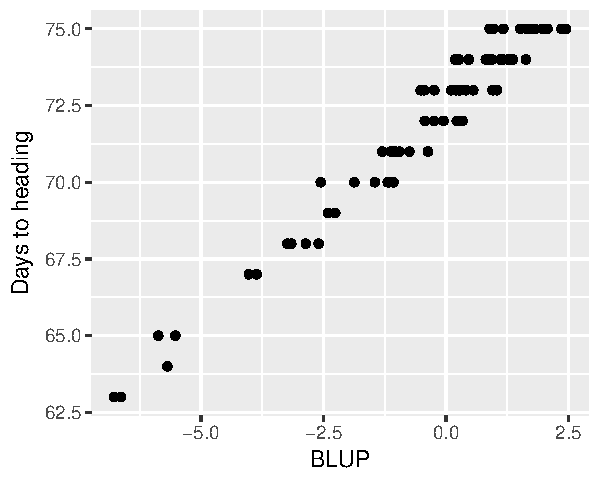
\includegraphics[width=.48\linewidth]{thesis_files/figure-latex/other-blup-viz2-2} }\newline\subfloat[Days to anthesis\label{fig:other-blup-viz2-3}]{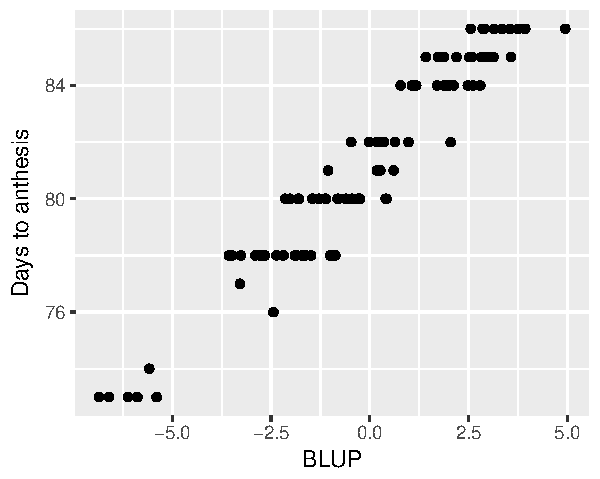
\includegraphics[width=.48\linewidth]{thesis_files/figure-latex/other-blup-viz2-3} }

}

\caption{Scatterplot of observed versus BLUP values of plant's morphological, architectural and phenological traits (...continued)}\label{fig:other-blup-viz2}
\end{figure}
\begin{figure}[H]

{\centering \subfloat[Plant height\label{fig:other-dotplot1-1}]{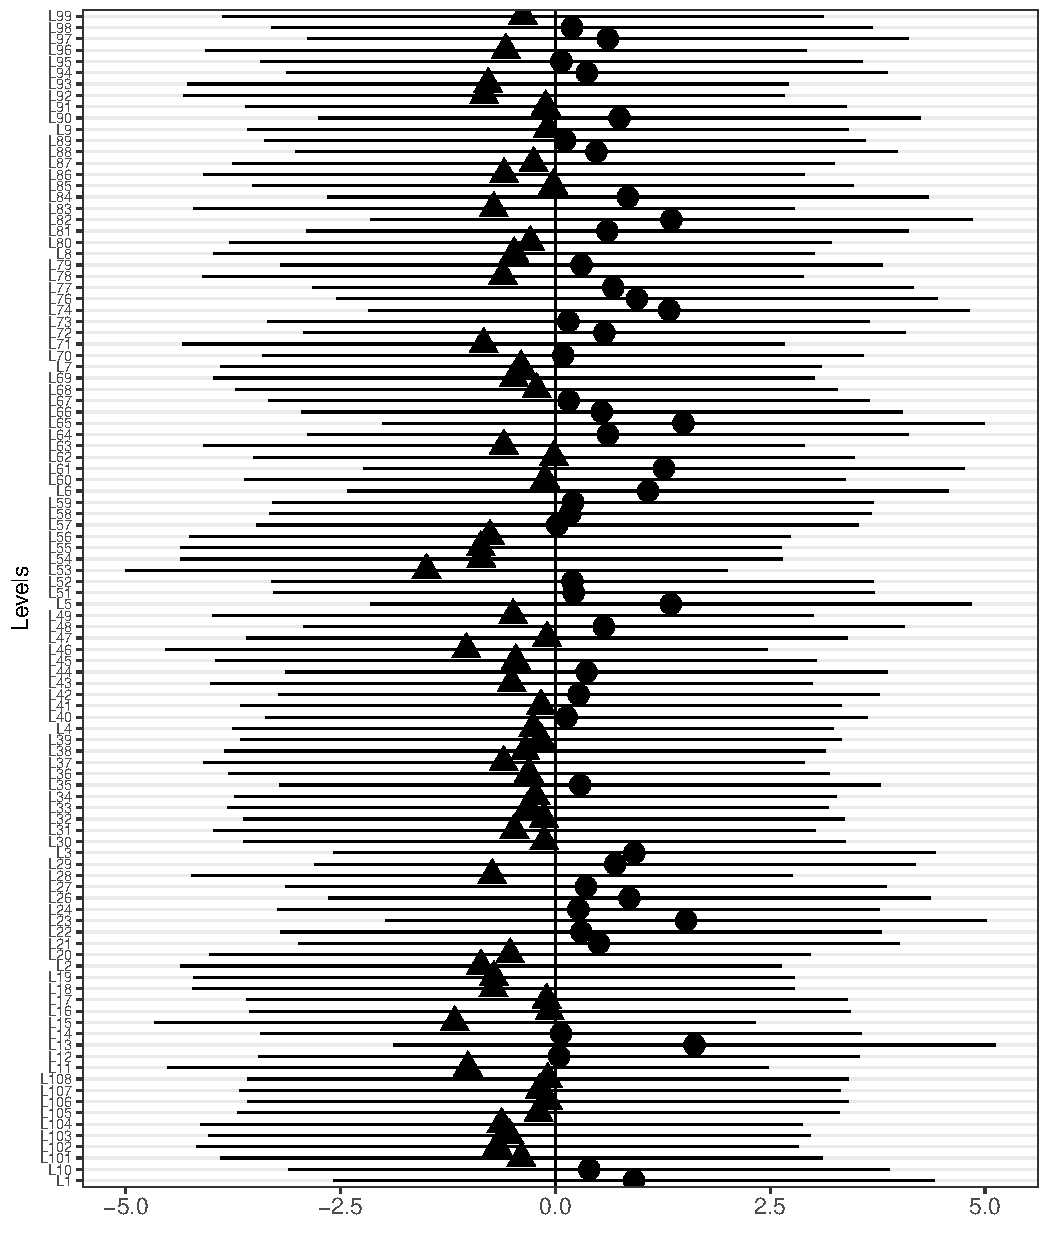
\includegraphics[width=.48\linewidth]{thesis_files/figure-latex/other-dotplot1-1} }\subfloat[Flag leaf area\label{fig:other-dotplot1-2}]{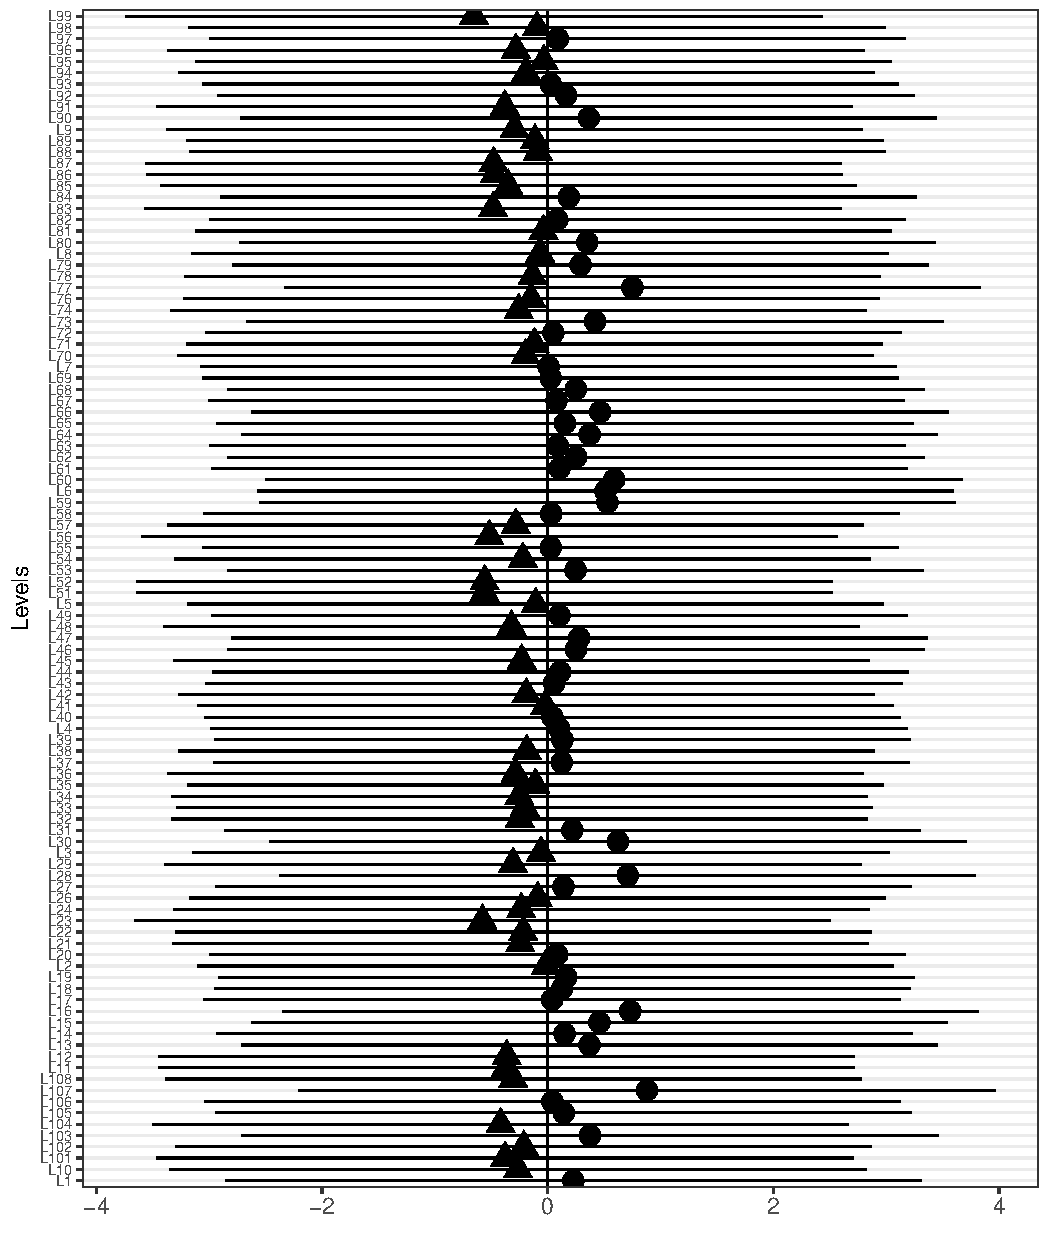
\includegraphics[width=.48\linewidth]{thesis_files/figure-latex/other-dotplot1-2} }\newline\subfloat[SPADI (Zadok's stage 65)\label{fig:other-dotplot1-3}]{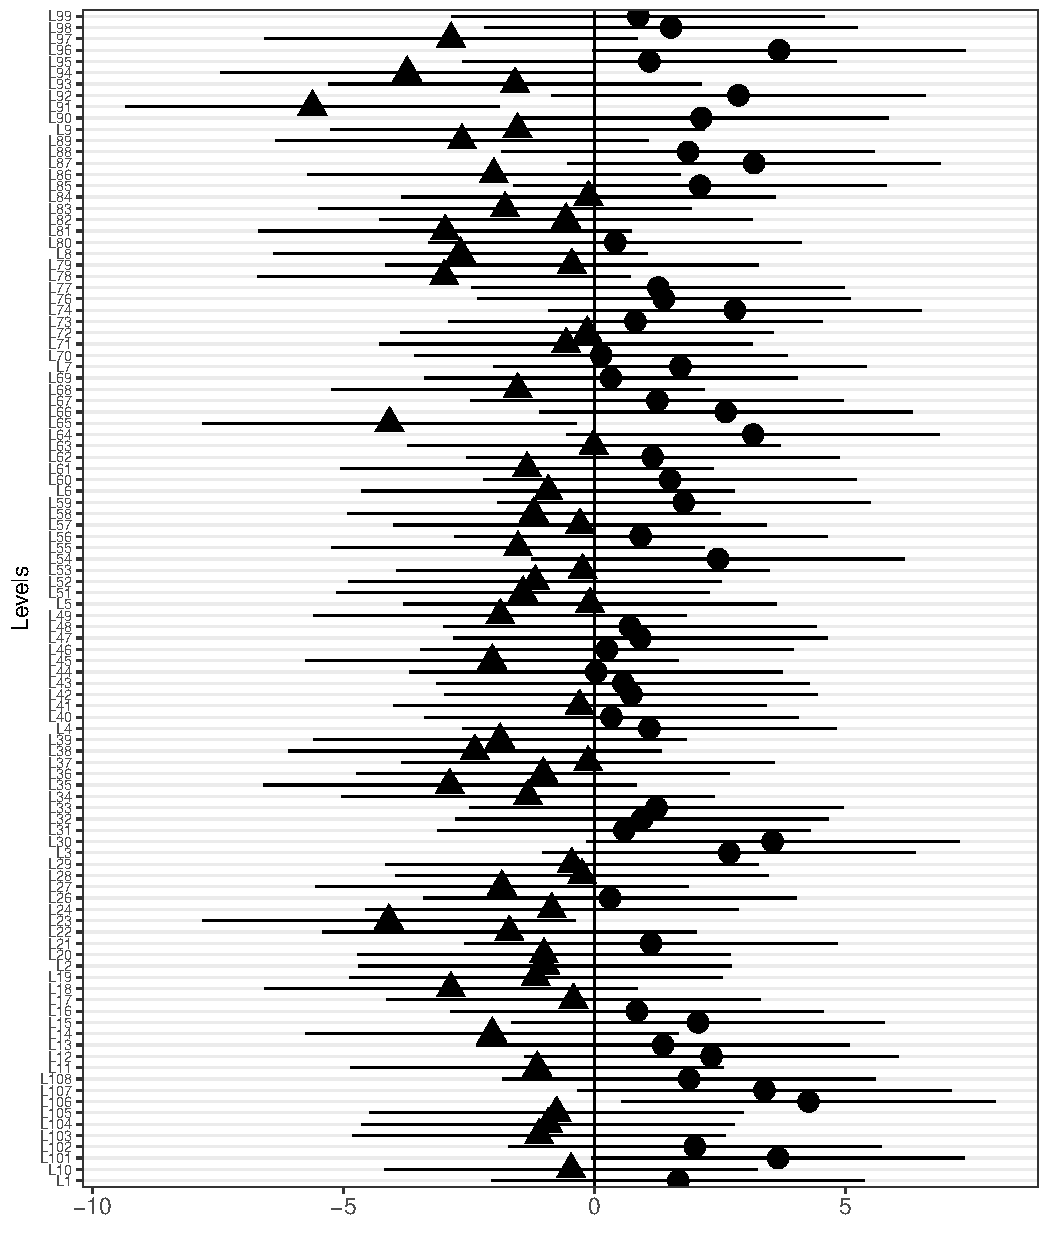
\includegraphics[width=.48\linewidth]{thesis_files/figure-latex/other-dotplot1-3} }\subfloat[SPADII (Zadok's stage 85)\label{fig:other-dotplot1-4}]{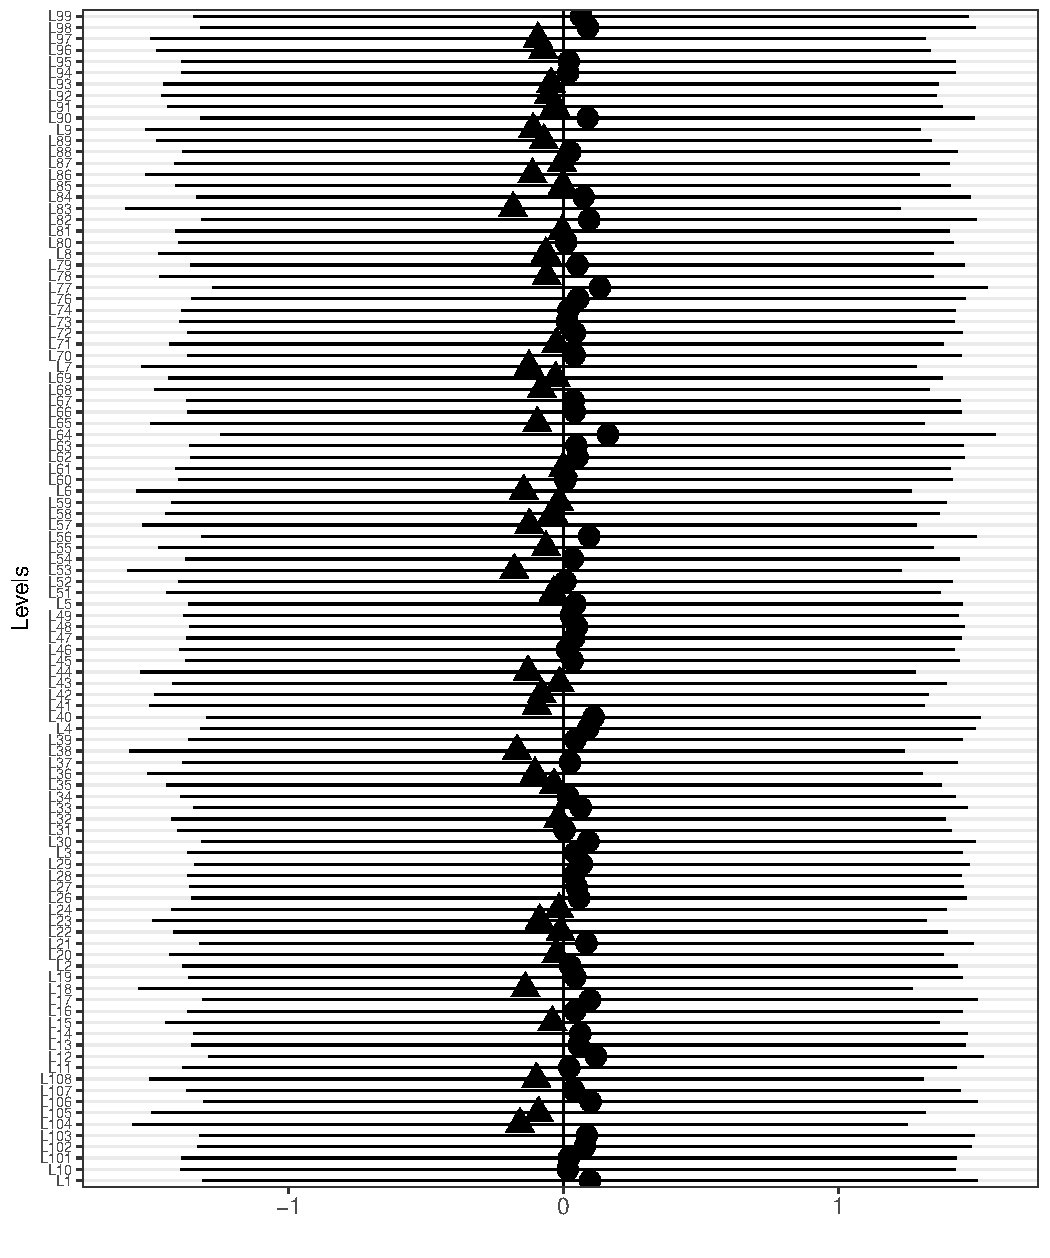
\includegraphics[width=.48\linewidth]{thesis_files/figure-latex/other-dotplot1-4} }

}

\caption{Random effect estimates of plant's morphological, architectural and phenological traits of entry genotypes}\label{fig:other-dotplot1}
\end{figure}
\begin{figure}[H]

{\centering \subfloat[Canopy temperature depression (CTD)\label{fig:other-dotplot2-1}]{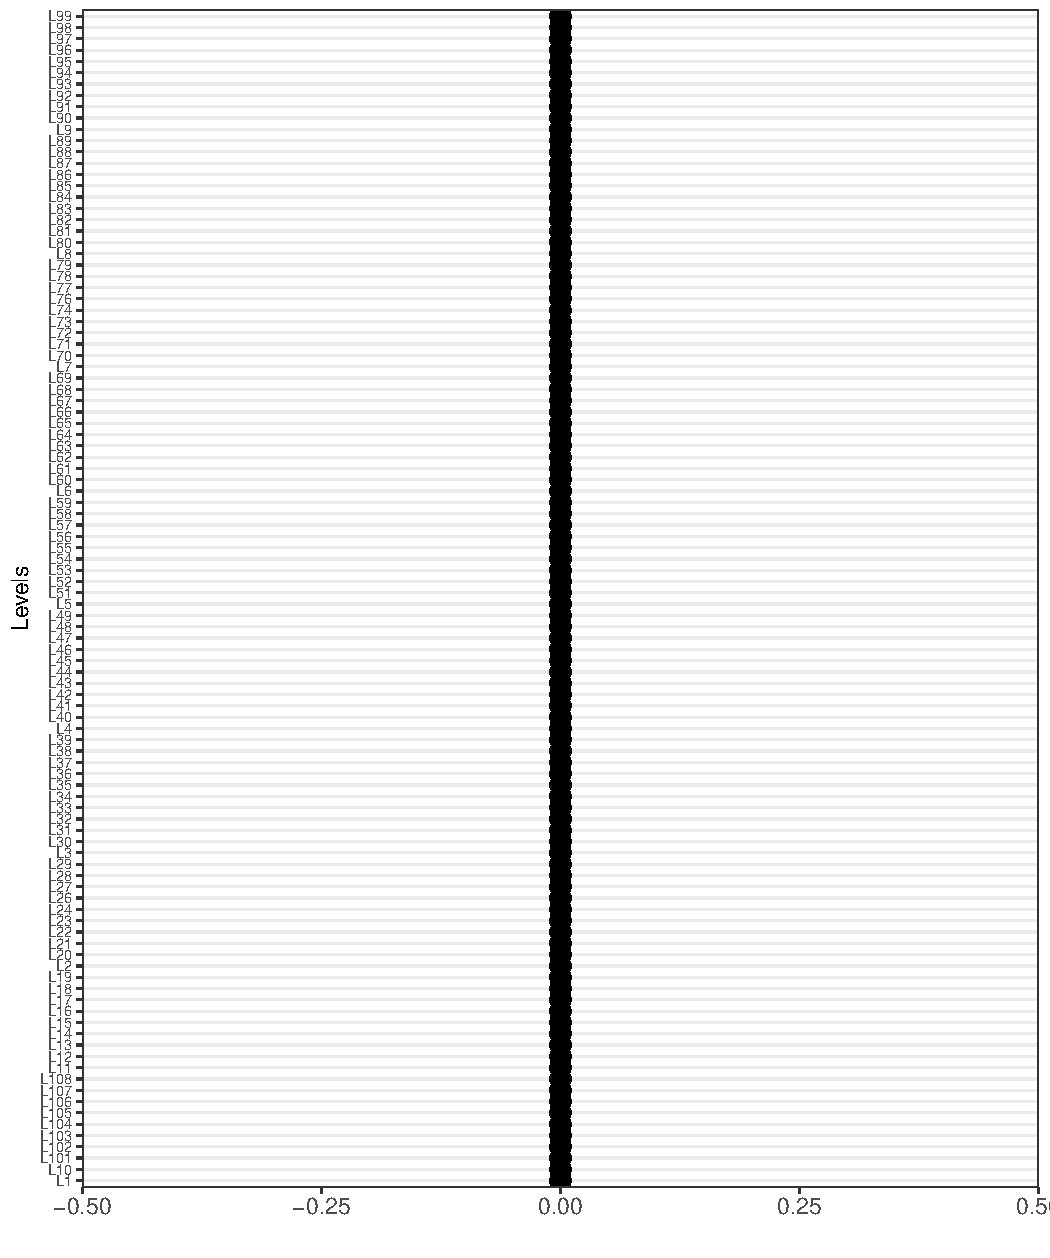
\includegraphics[width=.48\linewidth]{thesis_files/figure-latex/other-dotplot2-1} }\subfloat[Days to heading\label{fig:other-dotplot2-2}]{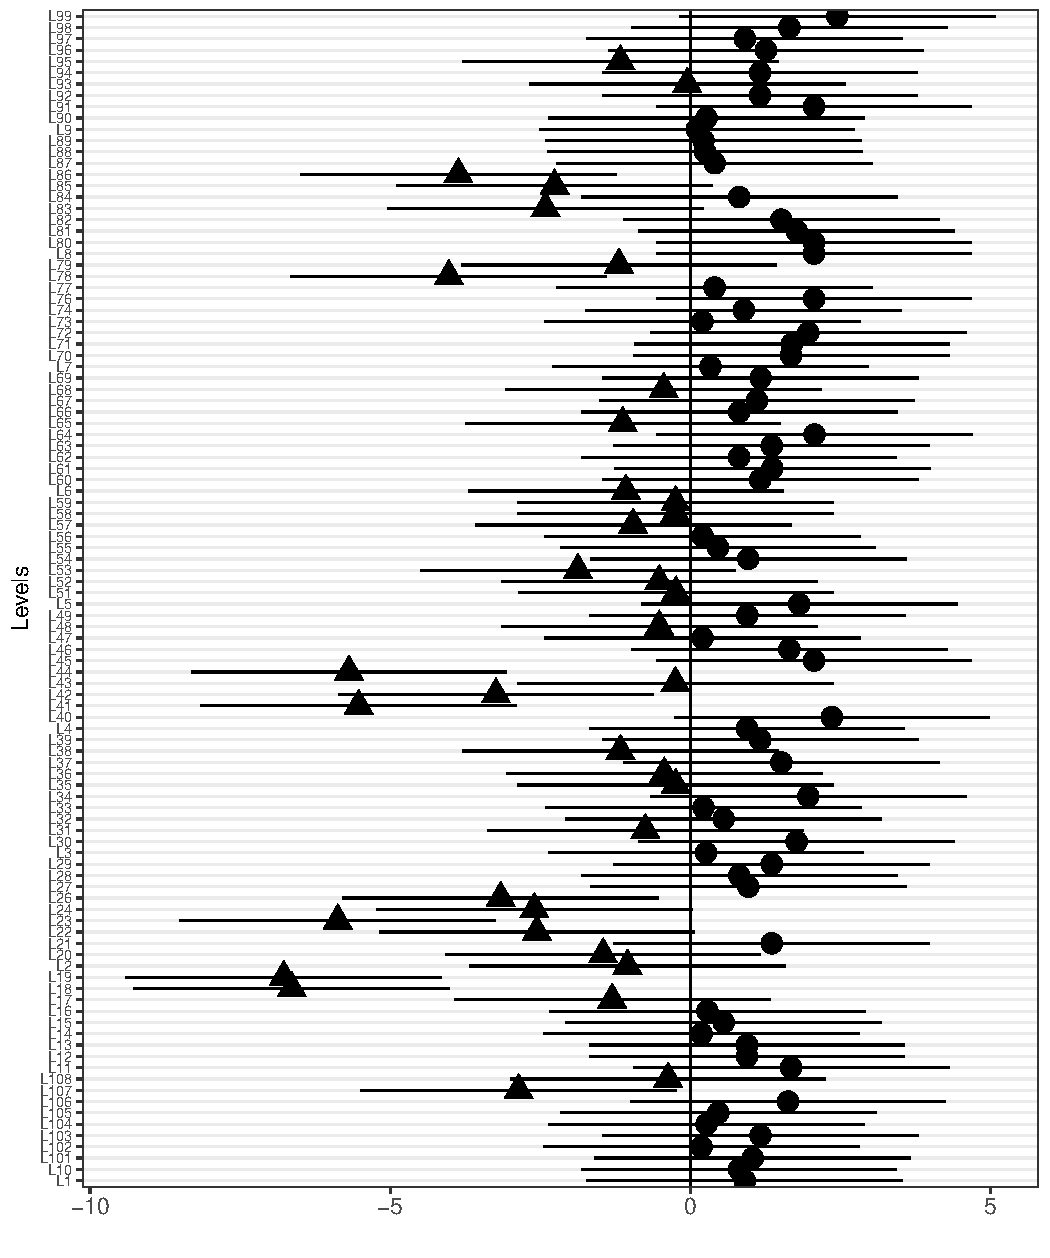
\includegraphics[width=.48\linewidth]{thesis_files/figure-latex/other-dotplot2-2} }\newline\subfloat[Days to anthesis\label{fig:other-dotplot2-3}]{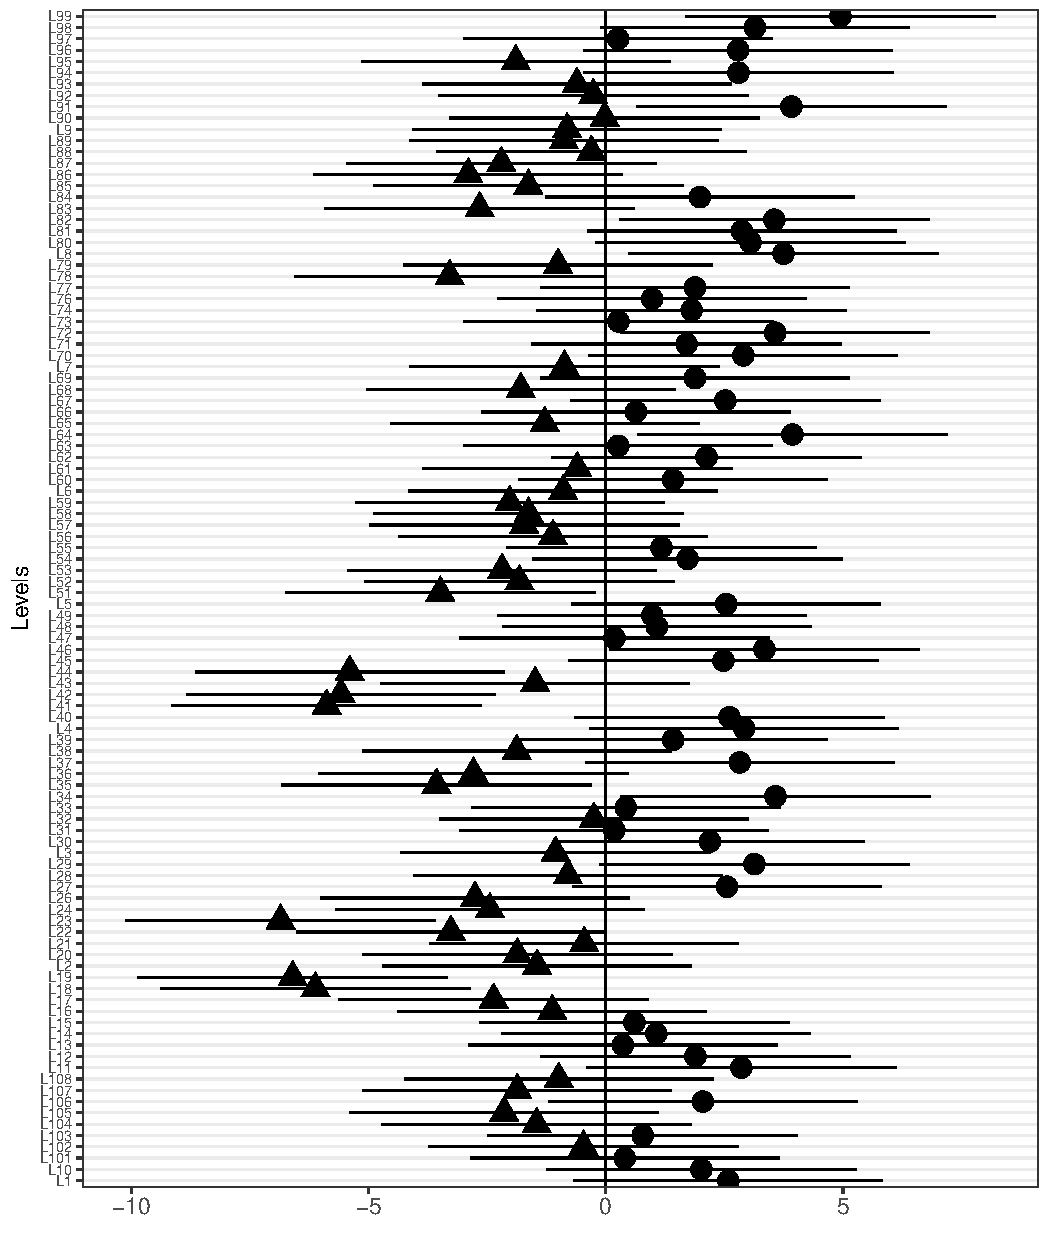
\includegraphics[width=.48\linewidth]{thesis_files/figure-latex/other-dotplot2-3} }

}

\caption{Random effect estimates of plant's morphological, architectural and phenological traits of entry genotypes (...continued)}\label{fig:other-dotplot2}
\end{figure}
\clearpage

\hypertarget{yield-prediction-using-leaf-health}{%
\section{Yield prediction using leaf health}\label{yield-prediction-using-leaf-health}}

A model approximating yield as a linear function of fixed effect terms for leaf health traits and random terms for blocking structure was formulated and ran. Along with model summary, effects estimates were obtained and coefficient of determination calculated based on the likelihood-ratio test (improvement from null (intercept only) model to the fitted model) (Magee, 1990).

\hypertarget{stepwise-variable-selection}{%
\subsection{Stepwise variable selection}\label{stepwise-variable-selection}}

For determining influencial variables among the candidates, stepwise variable selection was performed from a set of possible models. Table \ref{tab:fixed-terms-kept} and Table \ref{tab:rand-terms-kept} summarize which fixed and random effects variables, respectively, had or did not have significant influence in yield determination.

\begingroup\fontsize{10}{12}\selectfont
\begin{longtable}[t]{cccccccc}
\caption{\label{tab:fixed-terms-kept}ANOVA of fixed effect model terms with indication of significance of variables}\\
\toprule
\textbf{Trait variables} & \textbf{Sum Sq} & \textbf{Mean Sq} & \textbf{NumDF} & \textbf{DenDF} & \textbf{F.value} & \textbf{elim.num} & \textbf{Pr(>F)}\\
\midrule
\endfirsthead
\caption[]{\label{tab:fixed-terms-kept}ANOVA of fixed effect model terms with indication of significance of variables \textit{(continued)}}\\
\toprule
\textbf{Trait variables} & \textbf{Sum Sq} & \textbf{Mean Sq} & \textbf{NumDF} & \textbf{DenDF} & \textbf{F.value} & \textbf{elim.num} & \textbf{Pr(>F)}\\
\midrule
\endhead
\
\endfoot
\bottomrule
\endlastfoot
SPADII & 0.016 & 0.016 & 1 & 170.3 & 0.065 & 1 & 0.798\\
Disease Z75 & 0.120 & 0.120 & 1 & 188.8 & 0.484 & 2 & 0.487\\
Greenness Z85 & 0.220 & 0.220 & 1 & 190.0 & 0.890 & 3 & 0.347\\
Check genotypes & 4.416 & 1.104 & 4 & 27.9 & 4.471 & kept & 0.006\\
Greenness Z65 & 4.385 & 4.385 & 1 & 170.4 & 17.755 & kept & 0.000\\
Greenness Z75 & 5.322 & 5.322 & 1 & 190.5 & 21.552 & kept & 0.000\\
LAUG 65\_75 & 18.945 & 18.945 & 1 & 188.1 & 76.717 & kept & 0.000\\
SPADI & 3.134 & 3.134 & 1 & 187.2 & 12.689 & kept & 0.000\\*
\end{longtable}
\endgroup{}

\begingroup\fontsize{10}{12}\selectfont
\begin{longtable}[t]{ccccc}
\caption{\label{tab:rand-terms-kept}ANOVA of random effect model terms with indication of significance of variables}\\
\toprule
\textbf{Random variables} & \textbf{Chi.sq} & \textbf{Chi.DF} & \textbf{elim.num} & \textbf{p.value}\\
\midrule
\endfirsthead
\caption[]{\label{tab:rand-terms-kept}ANOVA of random effect model terms with indication of significance of variables \textit{(continued)}}\\
\toprule
\textbf{Random variables} & \textbf{Chi.sq} & \textbf{Chi.DF} & \textbf{elim.num} & \textbf{p.value}\\
\midrule
\endhead
\
\endfoot
\bottomrule
\endlastfoot
Nested col & 0.000 & 1 & 1 & 1.000\\
Rowgroup x Colgroup & 0.000 & 1 & 2 & 1.000\\
Nested row & 0.061 & 1 & 3 & 0.804\\
Rowgroup & 1.556 & 1 & 4 & 0.212\\
Colgroup & 8.560 & 1 & kept & 0.003\\
Line genotypes & 5.116 & 1 & kept & 0.024\\*
\end{longtable}
\endgroup{}

Stepwise variable selection and backward elimination of a mixed model with response variable yield suggests that, aside from the genotype effects, fixed effects of leaf health and canopy related traits significantly affect the yield (based on both, P-values calculated from F-test by Sattethwaite's approximation and AIC (Mazerolle, 2004; Wagenmakers \& Farrell, 2004) drop in the single term deletions of fixed effects terms in the model). In particular leaf greenness scores at Zadok's stage 65 and 75, LAUG value during Zadok's stage 65 and 75 and relative leaf chlorophyll content (SPADI) at Zadok's stage 65.

\hypertarget{efficiency-of-yield-prediction}{%
\subsection{Efficiency of yield prediction}\label{efficiency-of-yield-prediction}}

The coefficient of determination of full model (squared correlation coefficient between observed and fitted values) was 0.794. Similarly, accounting for random effects, including all blocking and treatment structures, \(R^2\) value of fixed effects terms (i.e.~proportion of variance explained by leaf health traits) is 0.393.

Using relative efficiency measure: indicates the decrease in error variance with additional terms in alternative model (with leaf health traits) over null the model (with random terms only), approximate gain in efficiency with the use of leaf health in estimating yield was almost 51.803\(\%\).

Top ten best performing entry genotypes based on fitted yield (BLUPs) ranking with their yield estimates are shown in Table \ref{tab:top-entry-genotypes}.

\begingroup\fontsize{10}{12}\selectfont
\begin{longtable}[t]{>{\centering\arraybackslash}p{2.0cm}>{\centering\arraybackslash}p{2.0cm}c}
\caption{\label{tab:top-entry-genotypes}Top ten best performing genotypes with respect to estimated yields}\\
\toprule
\textbf{Entry genotype} & \textbf{Estimated yield} & \textbf{Genotype}\\
\midrule
\endfirsthead
\caption[]{\label{tab:top-entry-genotypes}Top ten best performing genotypes with respect to estimated yields \textit{(continued)}}\\
\toprule
\textbf{Entry genotype} & \textbf{Estimated yield} & \textbf{Genotype}\\
\midrule
\endhead
\
\endfoot
\bottomrule
\endlastfoot
L71 & 4.50 & TRCH/SRTU//KACHU/3/KINGBIRD \#1\\
L67 & 4.38 & WHEAR/SOKOLL/4/PASTOR//MILAN/KAUZ/3/BAV92\\
L85 & 4.28 & MUNAL \#1*2/4/HUW234+LR34/PRINIA//PBW343*2/...\\
L106 & 4.22 & PFAU/MILAN//TROST/3/MUNAL \#1/4/PFAU/MILAN//...\\
L92 & 4.08 & ROLF07/KINGBIRD \#1//MUNAL \#1\\
L87 & 3.98 & MUNAL \#1*2/4/HUW234+LR34/PRINIA//PBW343*2/...\\
L43 & 3.95 & KACHU*2/PANDORA\\
L1 & 3.94 & MUNAL \#1\\
L84 & 3.93 & NL971*2/MUU\\
L105 & 3.89 & BABAX/LR42//BABAX*2/4/SNI/TRAP\#1/3/KAUZ*2/...\\*
\end{longtable}
\endgroup{}

\hypertarget{correlation-between-numeric-variables}{%
\section{Correlation between numeric variables}\label{correlation-between-numeric-variables}}

\blandscape
\begin{table}

\caption{\label{tab:plot-starred-corr}Correlation coefficients of numeric response variables observed in study}
\centering
\resizebox{\linewidth}{!}{
\fontsize{12}{14}\selectfont
\begin{threeparttable}
\begin{tabular}[t]{>{\raggedright\arraybackslash}p{0.12\textwidth}>{\raggedright\arraybackslash}p{0.12\textwidth}>{\raggedright\arraybackslash}p{0.12\textwidth}>{\raggedright\arraybackslash}p{0.12\textwidth}>{\raggedright\arraybackslash}p{0.12\textwidth}>{\raggedright\arraybackslash}p{0.12\textwidth}>{\raggedright\arraybackslash}p{0.12\textwidth}>{\raggedright\arraybackslash}p{0.12\textwidth}>{\raggedright\arraybackslash}p{0.12\textwidth}lllllllll}
\toprule
\textbf{ } & \textbf{Yild} & \textbf{Paen} & \textbf{ThWt} & \textbf{Gran} & \textbf{Efer} & \textbf{Di75} & \textbf{Gr65} & \textbf{Gr75} & \textbf{Gr85} & \textbf{La75} & \textbf{La85} & \textbf{Plht} & \textbf{Lar} & \textbf{Ctd} & \textbf{Spdi} & \textbf{Spii} & \textbf{Daad}\\
\midrule
Yild &  &  &  &  &  &  &  &  &  &  &  &  &  &  &  &  & \\
Paen & 0.13 &  &  &  &  &  &  &  &  &  &  &  &  &  &  &  & \\
ThWt & 0.18* & -0.12 &  &  &  &  &  &  &  &  &  &  &  &  &  &  & \\
Gran & 0.32**** & 0.41**** & -0.06 &  &  &  &  &  &  &  &  &  &  &  &  &  & \\
Efer & 0.56**** & -0.06 & -0.01 & -0.03 &  &  &  &  &  &  &  &  &  &  &  &  & \\
\addlinespace
Di75 & -0.07 & -0.17* & 0.03 & -0.05 & -0.06 &  &  &  &  &  &  &  &  &  &  &  & \\
Gr65 & -0.10 & -0.09 & 0.06 & -0.01 & 0.10 & -0.14* &  &  &  &  &  &  &  &  &  &  & \\
Gr75 & 0.10 & 0.20** & -0.12 & 0.18** & -0.19** & -0.18** & -0.07 &  &  &  &  &  &  &  &  &  & \\
Gr85 & 0.06 & 0.12 & -0.04 & 0.07 & -0.10 & -0.15* & 0.37**** & 0.77**** &  &  &  &  &  &  &  &  & \\
La75 & 0.34**** & 0.19** & -0.10 & 0.20** & 0.07 & -0.16* & 0.17** & 0.82**** & 0.75**** &  &  &  &  &  &  &  & \\
\addlinespace
La85 & 0.08 & 0.12 & -0.01 & 0.02 & -0.16* & -0.14* & 0.13 & 0.87**** & 0.85**** & 0.76**** &  &  &  &  &  &  & \\
Plht & -0.10 & 0.09 & -0.12 & 0.05 & -0.11 & -0.09 & 0.00 & 0.11 & 0.12 & 0.07 & 0.06 &  &  &  &  &  & \\
Lar & -0.04 & 0.18** & 0.05 & 0.10 & -0.02 & -0.08 & -0.11 & 0.10 & 0.03 & 0.08 & 0.07 & 0.11 &  &  &  &  & \\
Ctd & 0.08 & -0.19** & 0.07 & -0.05 & 0.13* & -0.10 & 0.00 & -0.20** & -0.14* & -0.17** & -0.15* & 0.03 & -0.02 &  &  &  & \\
Spdi & 0.22** & 0.11 & 0.13 & 0.16* & -0.03 & -0.22** & 0.10 & 0.18** & 0.18** & 0.19** & 0.19** & -0.11 & 0.04 & -0.08 &  &  & \\
\addlinespace
Spii & 0.05 & 0.26**** & -0.02 & 0.14* & 0.02 & -0.41**** & 0.05 & 0.17** & 0.14* & 0.14* & 0.15* & 0.23** & 0.11 & 0.08 & 0.26**** &  & \\
Daad & -0.13 & -0.07 & 0.25** & -0.12 & 0.04 & -0.06 & 0.30**** & -0.45**** & -0.17** & -0.29**** & -0.31**** & 0.11 & 0.07 & 0.18** & 0.13* & 0.24** & \\
Dath & -0.13 & -0.11 & 0.23** & -0.18** & 0.07 & -0.10 & 0.29**** & -0.45**** & -0.17** & -0.29**** & -0.29**** & 0.08 & 0.08 & 0.24** & 0.09 & 0.26**** & 0.93****\\
\bottomrule
\end{tabular}
\begin{tablenotes}
\item \textit{Note: } 
\item p < .0001: **** ; p < .001: *** ; p < .01: ** ; p < .05: * 
                       \newline Yild: Yield, Paen: Panicle length, 
                       \newline ThWt: Thousand kernel weight, Gran: Number of grains per panicle,
                       \newline Efer: Number of effective tillers, Di75: Disease score at Z75, 
                       \newline Gr65: Greenness score at Z65, Gr75: Greenness score at Z75, 
                       \newline Gr85: Greenness score at Z85, La75: LAUG score at Z75, 
                       \newline La85: LAUG score at Z85, Plht: Plant height, 
                       \newline Laar: Leaf area, Cttd: Canopy temperature depression, 
                       \newline Spdi: SPAD score at Z65, Spii: SPAD score at Z85, 
                       \newline Daad: Days to heading
\end{tablenotes}
\end{threeparttable}}
\end{table}
\elandscape

Pairwise test of pearson's correlation coefficients suggest a significant positive association of LAUG value during Zadok's stage 65 and 75 and the yield. Besides that, relative leaf chlorophyll content of the leaves (SPAD) recorded at Zadok's stage 65 are also significantly positively correlated with the yield. To the contrary, LAUG during Zadok's stage 65 was, with high degree of significant positive correlation, associated with the yield. This potentially implies that, a sharp drop in leaf greenness values right after flowering might be beneficial for yield formation, particularly to the number of grains per panicles.

No direct correlation to yield was apparent for other leaf health and traits characterizing canopy architecture. Major yield component traits associated with the yield were (in the decreasing order of significance) Number of effective tillers, Number of grains per panicle and the Thousand kernel weight. In addition, a higher relative chlorophyll content and a larger leaf surface area are implicated in longer panicles, although panicle length on itself is not significantly associated with the yield of the crop.

Several leaf health and canopy related traits had significant correlation with each other, for example, number of heading and flowering days for genotypes showed negative correlation with the decline in leaf greenness values, at both the early and latter stages of the life cycle. This potentially implies that, genotypes which flower early show higher drop in chlorophyll contents and reach to senescence earlier.

Likewise, certain phenological traits of interest in most selection programmes like days to heading and days to anthesis were significantly positively correlated with a particular yield component trait -- thousand kernel weight, and the latter is even negatively correlated to the number of grains per panicle.

\hypertarget{principal-component-analysis}{%
\section{Principal component analysis}\label{principal-component-analysis}}
\begin{figure}[H]

{\centering 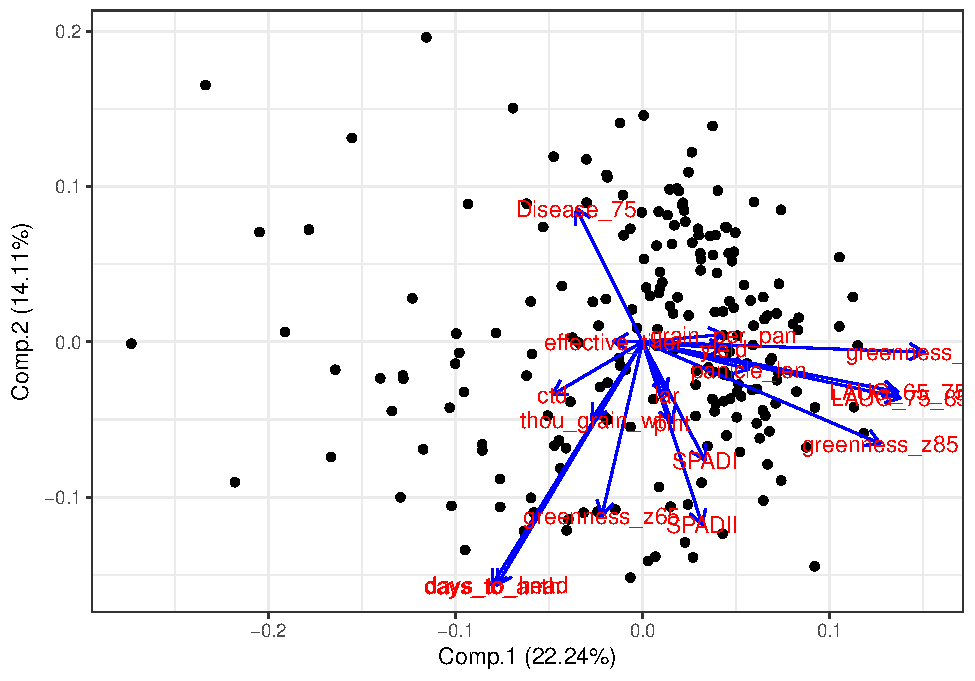
\includegraphics{thesis_files/figure-latex/principal-component-viz-1} 

}

\caption{PCA biplot showing first two principal components}\label{fig:principal-component-viz}
\end{figure}
The principal component analysis of continuous multivariate response shows that first two principal components explain 35.17\% variation. This is depicted in the Figure \ref{fig:principal-component-viz}. Table \ref{tab:principal-component-summary} shows summary of principal component analysis (Top ten principal components are shown with corresponding measures of proportionate variance and standard deviation of principal axes).

For the first principal component axis (PC1), most variables have positive values (All except plant height, canopy temperature depression, disease score and the number of effective tillers triats). Thus, most variables are positively correlated between each other. Most leaf health related and phenological traits, including greenness scores of two latter stages, LAUG values and the days to heading and anthesis traits, constrain the PC1 eigenvector (based on a large magnitude of variable eigenvalue loadings) (Table \ref{tab:principal-component-loadings}). Interestingly, the variability accounted for by this PC axis is different from that of the PC2 and PC3 (latter captures 10.3\% variation). Traits related to yield have higher factor variable loadings in PC3, amongst which yield \emph{per se} has the highest, while the number of effective tillers and the number of grains per panicle also contrain the third eigenvector. The scoring for disease contrasts itself in PC2. Also, all yield related traits can be seen as being positively correlated in the PC3 axis. Similarly, the indication of negative correlation between the days to heading and anthesis and the leaf greenness related traits corroborates the earlier speculation that genotypes that flower early are also characterized by earlier signs of drop in chlorophyll contents, and therefore reach to the senescence earlier.
\begin{table}[H]

\caption{\label{tab:principal-component-summary}Summary of principal component analysis with measures of variation explained by top ten principal axes}
\centering
\fontsize{11}{13}\selectfont
\begin{tabular}[t]{lcccccccccc}
\toprule
\textbf{ } & \textbf{PC1} & \textbf{PC2} & \textbf{PC3} & \textbf{PC4} & \textbf{PC5} & \textbf{PC6} & \textbf{PC7} & \textbf{PC8} & \textbf{PC9} & \textbf{PC10}\\
\midrule
Standard deviation & 2.00 & 1.59 & 1.36 & 1.30 & 1.12 & 1.03 & 1.02 & 0.92 & 0.87 & 0.82\\
Proportion of Variance & 0.22 & 0.14 & 0.10 & 0.09 & 0.07 & 0.06 & 0.06 & 0.05 & 0.04 & 0.04\\
Cumulative Proportion & 0.22 & 0.36 & 0.47 & 0.56 & 0.63 & 0.69 & 0.75 & 0.80 & 0.84 & 0.87\\
\bottomrule
\end{tabular}
\end{table}
\begin{table}[H]

\caption{\label{tab:principal-component-loadings}PCA factor loadings of top three principal components on variables for each of the numeric response variables observed in study}
\centering
\fontsize{11}{13}\selectfont
\begin{tabular}[t]{cccc}
\toprule
\textbf{Variable} & \textbf{PC1} & \textbf{PC2} & \textbf{PC3}\\
\midrule
Yield & -0.135 & 0.014 & 0.630\\
Panicle Len & -0.176 & 0.055 & 0.154\\
Grain Per Pan & -0.134 & -0.015 & 0.333\\
Thou Grain Wt & 0.085 & 0.155 & 0.134\\
Effective Tiller & 0.048 & 0.000 & 0.512\\
Greenness Z65 & 0.068 & 0.349 & -0.091\\
Greenness Z75 & -0.468 & 0.021 & -0.114\\
Greenness Z85 & -0.395 & 0.204 & -0.163\\
Laug 65 75 & -0.424 & 0.100 & 0.091\\
Laug 75 85 & -0.428 & 0.112 & -0.161\\
Disease 75 & 0.110 & -0.267 & -0.065\\
Spadi & -0.104 & 0.237 & 0.206\\
Spadii & -0.099 & 0.366 & 0.068\\
Ctd & 0.150 & 0.106 & 0.148\\
Plht & -0.049 & 0.162 & -0.176\\
Lar & -0.040 & 0.105 & -0.010\\
Days To Head & 0.242 & 0.487 & -0.028\\
Days To Anth & 0.250 & 0.488 & -0.042\\
\bottomrule
\end{tabular}
\end{table}
\begin{figure}[H]

{\centering 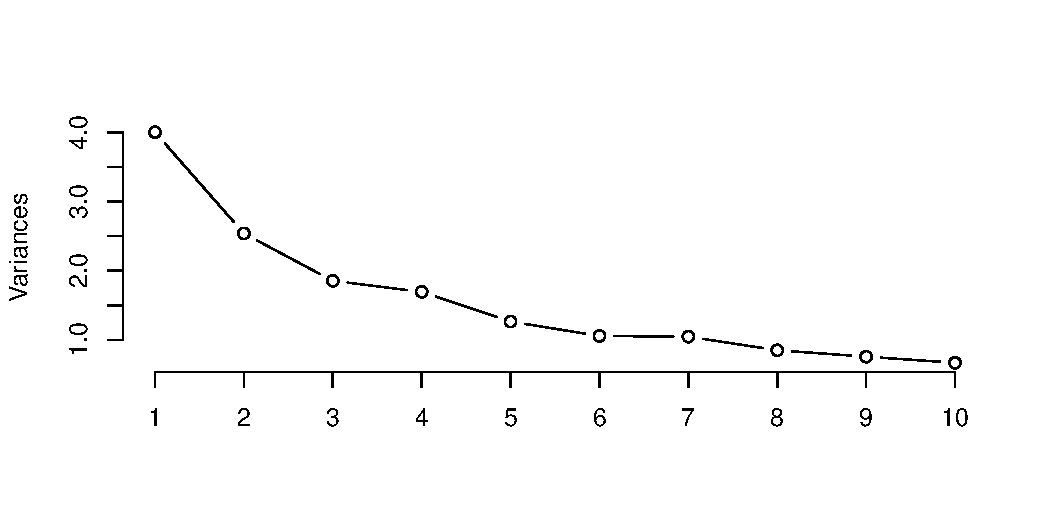
\includegraphics[width=0.80\linewidth]{thesis_files/figure-latex/screeplot-1} 

}

\caption{Principal component analysis screeplot of plants' trait responses}\label{fig:screeplot}
\end{figure}
The PCA screeplot (Figure \ref{fig:screeplot}) shows the decay of variability (y-axis) with increasing numbers of independent principal components (x-axis) used for decomposing observed variability in the data. A sharp drop in proportion of total variance explained by the PCs is only realized after linear combination of 6-7 PCs. This indicates that data inherently is best resolved into large number of dimensions. This seems to be true and features unique opportunity as well as challenge from the perspective of modeling and analysing of a field experiment while controlling for several extrinsic factors that might otherwise result in the problem of sparsity of data.

\hypertarget{discussion}{%
\chapter{Discussion}\label{discussion}}

\hypertarget{relationship-between-leaf-health-and-yield}{%
\section{Relationship between leaf health and yield}\label{relationship-between-leaf-health-and-yield}}

Four leaf health traits were identified with significant association to yield. Inspection of individual variance components reveals that for yield and yield component traits, blocking of plots into either factors, i.e row, column or superimposed row-colum, generally did not significantly reduce the error variance. However, thousand kernel weight was affected also by the variation along the column nested inside colum-group (increasing of effect along column 1 to 12). The finding is in accordance to the study of Neupane Adhikari, Wu, \& Caffe (2016), where significant estimates have been recovered by spatial modeling.

Also, the effect on disease rating of foliar disease complex due to blocking in nested column inside columngroup is characterized by a decreasing gradient along column rank one to rank twelve. This might provide an explaination for significant difference in thousand grain weight also along the the column blocks. As expected, the yield associated trait benefitted by the reduced disease pressure along the column block. In a multi-year study undertaken to identify definitive traits and their relative importance in improving resistance to Helminthosporium blight along with yield related traits, Sharma \& Duveiller (2003) reported similar negative correlation between resistance to foliar disease and the kernel weight.

However, genotypes which manifested a sharp drop in relative chlorophyll content of the flag leaf just after antheis and before milking stage generally gave higher yields. The drop in chlorophyll content has often been ascribed to drought tolerance, in which case a higher drop in chlorophyll content is associated with drought sensitivity (Khakwani et al., 2013) (authors used chlorophyll fluorescence extinction measurement as) and irrigated cultivars in general showed higher decline in chlorophyll content, under stress. In comparison, experimental condition of the field where genotypes were tested was irrigated prior to heading. Therefore, this might represent non-water-limiting/irrigated condition. This set of environmental conditions in combination with genotypic features that supress activated drought tolerance mechanism, might enable genotypes with higher LAUG values (\(120.1\) and \(92.18\), respectively for period between anthesis and medium milk and medium milk and soft dough stages) to better realize their potential yields.

Findings on the association of relative chlorophyll content and the decline in chlorophyll content with the yield in wheat extend that of Khakwani et al. (2013), where significant correlation between yield and the indicator of leaf chlorophyll have been reported. Current study highlights, in particular, the importance of leaf chlorophyll content and the rate of decline of greenness at early stages in reproductive phase of the crop (Wu, Tang, Li, Wu, \& Huang, 2015). For the leaf greenness trait at Z65, however leaving out the entry genotype ``PRL/2*PAS-TOR/4/CHOIX/STAR/3/HE1/3*CNO79//\ldots{}'', which showed signs of severe depletion of green coloration of leaf early on life cycle, significant differences among entry genotypes could be inconclusive had the outlier been trimmed out.

\hypertarget{relationship-between-morphological-and-phenological-traits-and-yield}{%
\section{Relationship between morphological and phenological traits and yield}\label{relationship-between-morphological-and-phenological-traits-and-yield}}

With apparent positive but mild correlation between the days to heading and days to anthesis and the thousand kernel weight, the results from current study contrasts with observations by Duveiller, Kandel, Sharma, \& Shrestha (2005), in which they report a negative association of days to maturity with the thousand kernel weight. Extending to their findings, authors clarify that differences in the trait association were not always significant for early sown wheat (planted between 26 Nov to 11 Dec). Inferring on grounds that current study had sowing date prior to that reported in the study (23 March), it is imperative that negative association do not hold. The study, however, fails to link the relationship between days to heading/anthesis and yield, which has been observed with negative but weak correlation in some studies (Mohammadi, Sharifi, Karimizadeh, \& Shefazadeh, 2012).

\hypertarget{relationship-between-morphological-and-phenological-traits-and-leaf-health}{%
\section{Relationship between morphological and phenological traits and leaf health}\label{relationship-between-morphological-and-phenological-traits-and-leaf-health}}

Canopy architecture traits comprising plant height and flag leaf area had no significant correlation with any of the observed leaf health traits. To the contrast, canopy temperature depression showed weak negative correlation with the leaf greenness at Z75, suggesting that a larger drop in canopy temperature often occurs in genotypes with greenner leaves. Also, greenness of leaves and the relative chlorophyll content of leaves are both negatively associated with foliar disease specific symptoms. This phenomena along with correlated response to days to maturity has been explained as probable resistance mechanism to HLB in a study exploring selection index for HLB reistance in spring wheat (Duveiller et al., 2005).

Likewise, although negative correlation was found between days to heading and the foliar disease prevalence, it's significance of could not be validated. This is in contrast to the finding of Mahto (1999), who reported significant negative albeit weak correlation between the two variables.

\hypertarget{leaf-health-as-determinant-of-yield}{%
\section{Leaf health as determinant of yield}\label{leaf-health-as-determinant-of-yield}}

Decrease in error variance invariably adds to the heritability estimates and relative efficiency of a trait, thus maximizing chances of selecting true to the type genotypes (Bondalapati, Jenkins, McCarty, \& Wu, 2015). Almost 52\% reduction in the error variance was obtained by incorporating leaf health traits in the model. Similarly, leaf health traits can be ascribed to upto 39\% variation in yield estimates. Among the traits of interest are the LAUG decline during Z65 and Z75, greenness scores at both Z75 and Z65 and the relative chlorophyll content at Z65. In a study by (Benbella \& Paulsen, 1998) have also implied significant effect of greenness trait -- defined in context of late maturity stage as ``Stay green'' -- in yield determination and its association with foliar blight disease. However, significance of foliar blight complex disease in yield determination in experimental conditions of the present study was not evident. This is probably because environmental/spatial effects of disease were more relevant (as observed from significant columwise blocking) and the heterogeniety between blocks was much higher to directly ascribe yields levels. Also, comparing two distinct yield groups (one with high TKW and the other with low TKW) in a study of evaluating wheat genotypes, authors have reported no significant association of two yield groups and the disease response (AUDPC) under timely sown conditions (Sharma, Tiwary, \& Ortiz-Ferrara, 2008).

Application of mixed modeling procedures to field phenotyping in wide set of environmental conditions is justified in several previous studies (Qiao, Basford, DeLacy, \& Cooper, 2000; Smith, Cullis, \& Gilmour, 2001). Spatial covariate modeling along with leaf health also had beneficial effect on yield approximation, although exact quantification of effect estimates would require more advanced probabilistic techniques such as Jackknife resampling and bootstrapping (Wu et al., 2013; Wu, Jenkins, \& McCarty, 2010).

With respect to estimated yield, all check cultivars were superior to Aditya variety and no distinction could be made between Bhrikuti, Gautam and Tilottama genotypes. While with genotypic BLUP estimates, ranking of genotypes places following three genotypes (on decending order) on top: L71 (TRCH/SRTU-//KACHU/3/-KINGBIRD \#1), L67 (WHEAR/-SOKOLL/4/-PASTOR//MILAN/-KAUZ/3/B\ldots) and L85 (MUNAL \#1*2/4/-HUW234+LR34/PRINIA-//PBW3\ldots). Pedigree information of the entry genotypes at foremost ranks suggests that genotypes composed of ``MUNAL'' in their pedigree with higher order\footnote{Order of crossing is denoted by a number sandwiched between two backslash (`/')} crossings or recurrent crossing, preferably as female parent has tendency for better yields.

\hypertarget{conclusions}{%
\chapter*{Conclusions}\label{conclusions}}
\addcontentsline{toc}{chapter}{Conclusions}

Yield approximation, having significant role in genotype selection, could be much improved by adding leaf health factor in screening and evaluation programs. Likewise, even in classical breeding traits, i.e.~crop architecture such as plant height and canopy temperature depression, accuracy of phenotype based selection could be improved through adoption of better designs, which can address multiple sources of spatial heterogeniety in the field. In turn, these extraneous variation could be accounted for through mixed modeling procedures. Therefore, besides improving the precision of estimation with inclusion of leaf health traits, in particular greenness and relative chlorophyll content measures at early post-anthesis period, certain traits such as thousand kernel weight, plant height, flag leaf area, canopy temperature depression, days to heading and days to anthesis benefitted the most by modeling of spatial covariates.

\appendix

\hypertarget{i}{%
\chapter{I}\label{i}}

\textbf{Tables referenced in Chapter \ref{modeling-yield-and-yield-component-traits}:}
\begin{table}[H]

\caption{\label{tab:unnamed-chunk-3}\label{tab:lrt-yield}ANOVA table with likelihood ratio test for Yield}
\centering
\begin{tabular}[t]{>{\raggedright\arraybackslash}p{3.5cm}llllllll}
\toprule
term & df & AIC & BIC & logLik & deviance & statistic & Chi.Df & p.value\\
\midrule
Blocking factors & 7 & 442 & 465 & -214 & 428 &  &  & \\
Blocking factors + Entry genotypes & 8 & 440 & 467 & -212 & 424 & 3.68 & 1 & 0.055\\
Blocking factors + Check and entry genotypes & 12 & 434 & 474 & -205 & 410 & 14.41 & 4 & 0.006\\
\bottomrule
\end{tabular}
\end{table}
\begin{table}[H]

\caption{\label{tab:unnamed-chunk-3}\label{tab:lrt-netill}ANOVA table with likelihood ratio test for Number of effective tillers}
\centering
\begin{tabular}[t]{>{\raggedright\arraybackslash}p{3.5cm}llllllll}
\toprule
term & df & AIC & BIC & logLik & deviance & statistic & Chi.Df & p.value\\
\midrule
Blocking factors & 7 & 1573 & 1597 & -779 & 1559 &  &  & \\
Blocking factors + Entry genotypes & 8 & 1565 & 1593 & -775 & 1549 & 9.73 & 1 & 0.002\\
Blocking factors + Check and entry genotypes & 12 & 1538 & 1580 & -757 & 1514 & 35.15 & 4 & 0.000\\
\bottomrule
\end{tabular}
\end{table}
\begin{table}[H]

\caption{\label{tab:unnamed-chunk-3}\label{tab:lrt-tkw}ANOVA table with likelihood ratio test for Thousand kernel weight}
\centering
\begin{tabular}[t]{>{\raggedright\arraybackslash}p{3.5cm}llllllll}
\toprule
term & df & AIC & BIC & logLik & deviance & statistic & Chi.Df & p.value\\
\midrule
Blocking factors & 7 & 1216 & 1239 & -601 & 1202 &  &  & \\
Blocking factors + Entry genotypes & 8 & 1186 & 1212 & -585 & 1170 & 32.0 & 1 & 0.000\\
Blocking factors + Check and entry genotypes & 12 & 1184 & 1223 & -580 & 1160 & 10.3 & 4 & 0.036\\
\bottomrule
\end{tabular}
\end{table}
\begin{table}[H]

\caption{\label{tab:unnamed-chunk-3}\label{tab:lrt-gperpan}ANOVA table with likelihood ratio test for Number of grains per panicle}
\centering
\begin{tabular}[t]{>{\raggedright\arraybackslash}p{3.5cm}llllllll}
\toprule
term & df & AIC & BIC & logLik & deviance & statistic & Chi.Df & p.value\\
\midrule
Blocking factors & 7 & 946 & 969 & -466 & 932 &  &  & \\
Blocking factors + Entry genotypes & 8 & 936 & 962 & -460 & 920 & 12.4 & 1 & 0.000\\
Blocking factors + Check and entry genotypes & 12 & 932 & 972 & -454 & 908 & 11.6 & 4 & 0.021\\
\bottomrule
\end{tabular}
\end{table}
\begin{table}[H]

\caption{\label{tab:unnamed-chunk-3}\label{tab:lrt-panlen}ANOVA table with likelihood ratio test for Panicle length}
\centering
\begin{tabular}[t]{>{\raggedright\arraybackslash}p{3.5cm}llllllll}
\toprule
term & df & AIC & BIC & logLik & deviance & statistic & Chi.Df & p.value\\
\midrule
Blocking factors & 7 & 869 & 893 & -428 & 855 &  &  & \\
Blocking factors + Entry genotypes & 8 & 859 & 886 & -421 & 843 & 12.8 & 1 & 0.000\\
Blocking factors + Check and entry genotypes & 12 & 852 & 893 & -414 & 828 & 14.6 & 4 & 0.006\\
\bottomrule
\end{tabular}
\end{table}
\textbf{Tables referenced in Chapter \ref{modeling-leaf-health-traits}:}
\begin{table}[H]

\caption{\label{tab:unnamed-chunk-4}\label{tab:lrt-dis-score}ANOVA table with likelihood ratio test for Disease score at Zadok's stage 75}
\centering
\begin{tabular}[t]{>{\raggedright\arraybackslash}p{3.5cm}llllllll}
\toprule
term & df & AIC & BIC & logLik & deviance & statistic & Chi.Df & p.value\\
\midrule
Blocking factors & 7 & 871 & 895 & -428 & 857 &  &  & \\
Blocking factors + Entry genotypes & 8 & 856 & 884 & -420 & 840 & 16.6 & 1 & 0.000\\
Blocking factors + Check and entry genotypes & 12 & 850 & 892 & -413 & 826 & 13.9 & 4 & 0.008\\
\bottomrule
\end{tabular}
\end{table}
\begin{table}[H]

\caption{\label{tab:unnamed-chunk-4}\label{tab:lrt-greenness1}ANOVA table with likelihood ratio test for Flag leaf greenness score at Zadok's stage 65}
\centering
\begin{tabular}[t]{>{\raggedright\arraybackslash}p{3.5cm}llllllll}
\toprule
term & df & AIC & BIC & logLik & deviance & statistic & Chi.Df & p.value\\
\midrule
Blocking factors & 7 & 306 & 331 & -146 & 292 &  &  & \\
Blocking factors + Entry genotypes & 8 & 263 & 291 & -123 & 247 & 45.50 & 1 & 0.000\\
Blocking factors + Check and entry genotypes & 12 & 266 & 308 & -121 & 242 & 4.83 & 4 & 0.305\\
\bottomrule
\end{tabular}
\end{table}
\begin{table}[H]

\caption{\label{tab:unnamed-chunk-4}\label{tab:lrt-greenness2}ANOVA table with likelihood ratio test for Flag leaf greenness score at Zadok's stage 75}
\centering
\begin{tabular}[t]{>{\raggedright\arraybackslash}p{3.5cm}llllllll}
\toprule
term & df & AIC & BIC & logLik & deviance & statistic & Chi.Df & p.value\\
\midrule
Blocking factors & 7 & 867 & 891 & -426 & 853 &  &  & \\
Blocking factors + Entry genotypes & 8 & 699 & 727 & -341 & 683 & 169.8 & 1 & 0\\
Blocking factors + Check and entry genotypes & 12 & 674 & 716 & -325 & 650 & 32.8 & 4 & 0\\
\bottomrule
\end{tabular}
\end{table}
\begin{table}[H]

\caption{\label{tab:unnamed-chunk-4}\label{tab:lrt-greenness3}ANOVA table with likelihood ratio test for Flag leaf greenness score at Zadok's stage 85}
\centering
\begin{tabular}[t]{>{\raggedright\arraybackslash}p{3.5cm}llllllll}
\toprule
term & df & AIC & BIC & logLik & deviance & statistic & Chi.Df & p.value\\
\midrule
Blocking factors & 7 & 889 & 914 & -438 & 875 &  &  & \\
Blocking factors + Entry genotypes & 8 & 848 & 876 & -416 & 832 & 43.4 & 1 & 0.000\\
Blocking factors + Check and entry genotypes & 12 & 842 & 884 & -409 & 818 & 14.2 & 4 & 0.007\\
\bottomrule
\end{tabular}
\end{table}
\begin{table}[H]

\caption{\label{tab:unnamed-chunk-4}\label{tab:lrt-laug1}ANOVA table with likelihood ratio test for LAUG between Zadok's stage 65 and 75}
\centering
\begin{tabular}[t]{>{\raggedright\arraybackslash}p{3.5cm}llllllll}
\toprule
term & df & AIC & BIC & logLik & deviance & statistic & Chi.Df & p.value\\
\midrule
Blocking factors & 7 & 1828 & 1852 & -907 & 1814 &  &  & \\
Blocking factors + Entry genotypes & 8 & 1757 & 1785 & -871 & 1741 & 72.79 & 1 & 0.000\\
Blocking factors + Check and entry genotypes & 12 & 1759 & 1801 & -867 & 1735 & 6.22 & 4 & 0.184\\
\bottomrule
\end{tabular}
\end{table}
\begin{table}[H]

\caption{\label{tab:unnamed-chunk-4}\label{tab:lrt-laug2}ANOVA table with likelihood ratio test for LAUG between Zadok's stage 75 and 85}
\centering
\begin{tabular}[t]{>{\raggedright\arraybackslash}p{3.5cm}llllllll}
\toprule
term & df & AIC & BIC & logLik & deviance & statistic & Chi.Df & p.value\\
\midrule
Blocking factors & 7 & 2174 & 2199 & -1080 & 2160 &  &  & \\
Blocking factors + Entry genotypes & 8 & 2088 & 2116 & -1036 & 2072 & 88.6 & 1 & 0\\
Blocking factors + Check and entry genotypes & 12 & 2074 & 2116 & -1025 & 2050 & 21.6 & 4 & 0\\
\bottomrule
\end{tabular}
\end{table}
\textbf{Tables referenced in Chapter \ref{modeling-plant-morphological-architectural-and-phenological-traits}:}
\begin{table}[H]

\caption{\label{tab:unnamed-chunk-5}\label{tab:lrt-plht}ANOVA table with likelihood ratio test for Plant height}
\centering
\begin{tabular}[t]{>{\raggedright\arraybackslash}p{3.5cm}llllllll}
\toprule
term & df & AIC & BIC & logLik & deviance & statistic & Chi.Df & p.value\\
\midrule
Blocking factors & 7 & 1565 & 1589 & -775 & 1551 &  &  & \\
Blocking factors + Entry genotypes & 8 & 1567 & 1594 & -775 & 1551 & 0.0 & 1 & 1\\
Blocking factors + Check and entry genotypes & 12 & 1493 & 1534 & -734 & 1469 & 82.2 & 4 & 0\\
\bottomrule
\end{tabular}
\end{table}
\begin{table}[H]

\caption{\label{tab:unnamed-chunk-5}\label{tab:lrt-lar}ANOVA table with likelihood ratio test for Flag leaf surface area}
\centering
\begin{tabular}[t]{>{\raggedright\arraybackslash}p{3.5cm}llllllll}
\toprule
term & df & AIC & BIC & logLik & deviance & statistic & Chi.Df & p.value\\
\midrule
Blocking factors & 7 & 1676 & 1700 & -831 & 1662 &  &  & \\
Blocking factors + Entry genotypes & 8 & 1678 & 1706 & -831 & 1662 & 0.00 & 1 & 1.000\\
Blocking factors + Check and entry genotypes & 12 & 1678 & 1720 & -827 & 1654 & 7.68 & 4 & 0.104\\
\bottomrule
\end{tabular}
\end{table}
\begin{table}[H]

\caption{\label{tab:unnamed-chunk-5}\label{tab:lrt-spadi}ANOVA table with likelihood ratio test for SPAD at Zadok's stage 65}
\centering
\begin{tabular}[t]{>{\raggedright\arraybackslash}p{3.5cm}llllllll}
\toprule
term & df & AIC & BIC & logLik & deviance & statistic & Chi.Df & p.value\\
\midrule
Blocking factors & 7 & 1238 & 1262 & -612 & 1224 &  &  & \\
Blocking factors + Entry genotypes & 8 & 1230 & 1258 & -607 & 1214 & 9.59 & 1 & 0.002\\
Blocking factors + Check and entry genotypes & 12 & 1229 & 1271 & -603 & 1205 & 8.95 & 4 & 0.062\\
\bottomrule
\end{tabular}
\end{table}
\begin{table}[H]

\caption{\label{tab:unnamed-chunk-5}\label{tab:lrt-spadii}ANOVA table with likelihood ratio test for SPAD at Zadok's stage 75}
\centering
\begin{tabular}[t]{>{\raggedright\arraybackslash}p{3.5cm}llllllll}
\toprule
term & df & AIC & BIC & logLik & deviance & statistic & Chi.Df & p.value\\
\midrule
Blocking factors & 7 & 1608 & 1632 & -797 & 1594 &  &  & \\
Blocking factors + Entry genotypes & 8 & 1610 & 1638 & -797 & 1594 & 0 & 1 & 1\\
Blocking factors + Check and entry genotypes & 12 & 1597 & 1639 & -786 & 1573 & 21 & 4 & 0\\
\bottomrule
\end{tabular}
\end{table}
\begin{table}[H]

\caption{\label{tab:unnamed-chunk-5}\label{tab:lrt-ctd}ANOVA table with likelihood ratio test for Canopy temperature depression (CTD)}
\centering
\begin{tabular}[t]{>{\raggedright\arraybackslash}p{3.5cm}llllllll}
\toprule
term & df & AIC & BIC & logLik & deviance & statistic & Chi.Df & p.value\\
\midrule
Blocking factors & 7 & 794 & 819 & -390 & 780 &  &  & \\
Blocking factors + Entry genotypes & 8 & 779 & 807 & -382 & 763 & 17.2 & 1 & 0.000\\
Blocking factors + Check and entry genotypes & 12 & 775 & 817 & -375 & 751 & 12.4 & 4 & 0.015\\
\bottomrule
\end{tabular}
\end{table}
\begin{table}[H]

\caption{\label{tab:unnamed-chunk-5}\label{tab:lrt-dth}ANOVA table with likelihood ratio test for Days to heading}
\centering
\begin{tabular}[t]{>{\raggedright\arraybackslash}p{3.5cm}llllllll}
\toprule
term & df & AIC & BIC & logLik & deviance & statistic & Chi.Df & p.value\\
\midrule
Blocking factors & 7 & 1393 & 1417 & -689 & 1379 &  &  & \\
Blocking factors + Entry genotypes & 8 & 1192 & 1220 & -588 & 1176 & 202 & 1 & 0\\
Blocking factors + Check and entry genotypes & 12 & 1045 & 1087 & -511 & 1021 & 155 & 4 & 0\\
\bottomrule
\end{tabular}
\end{table}
\begin{table}[H]

\caption{\label{tab:unnamed-chunk-5}\label{tab:lrt-dta}ANOVA table with likelihood ratio test for Days to anthesis}
\centering
\begin{tabular}[t]{>{\raggedright\arraybackslash}p{3.5cm}llllllll}
\toprule
term & df & AIC & BIC & logLik & deviance & statistic & Chi.Df & p.value\\
\midrule
Blocking factors & 7 & 1427 & 1451 & -706 & 1413 &  &  & \\
Blocking factors + Entry genotypes & 8 & 1228 & 1255 & -606 & 1212 & 201.2 & 1 & 0\\
Blocking factors + Check and entry genotypes & 12 & 1150 & 1191 & -563 & 1126 & 85.9 & 4 & 0\\
\bottomrule
\end{tabular}
\end{table}
\hypertarget{ii}{%
\chapter{II}\label{ii}}

\textbf{Snapshot of all statistical packages and processing environment used in analysis and interpretation of data:}
\begin{verbatim}
R version 3.6.3 (2020-02-29)
Platform: x86_64-pc-linux-gnu (64-bit)
Running under: Ubuntu 16.04.6 LTS

Matrix products: default
BLAS:   /usr/lib/libblas/libblas.so.3.6.0
LAPACK: /usr/lib/lapack/liblapack.so.3.6.0

locale:
 [1] LC_CTYPE=en_US.UTF-8    LC_NUMERIC=C            LC_TIME=en_US          
 [4] LC_COLLATE=en_US.UTF-8  LC_MONETARY=en_US       LC_MESSAGES=en_US.UTF-8
 [7] LC_PAPER=en_US          LC_NAME=C               LC_ADDRESS=C           
[10] LC_TELEPHONE=C          LC_MEASUREMENT=en_US    LC_IDENTIFICATION=C    

attached base packages:
[1] stats     graphics  grDevices utils     datasets  methods   base     

other attached packages:
 [1] ggfortify_0.4.8     Hmisc_4.4-0         Formula_1.2-3      
 [4] survival_3.1-12     lattice_0.20-41     xtable_1.8-4       
 [7] lmerTest_3.1-2      lme4_1.1-21         Matrix_1.2-18      
[10] forcats_0.4.0       stringr_1.4.0       purrr_0.3.4        
[13] readr_1.3.1         tidyr_1.1.0         tibble_3.0.3       
[16] tidyverse_1.3.0     thesisdowndss_0.0.1 knitr_1.29         
[19] bookdown_0.20       ggplot2_3.3.2       dplyr_1.0.0        
[22] devtools_2.3.1      usethis_1.6.1      

loaded via a namespace (and not attached):
 [1] minqa_1.2.4         colorspace_1.4-1    ellipsis_0.3.1     
 [4] rprojroot_1.3-2     htmlTable_1.13.3    base64enc_0.1-3    
 [7] fs_1.4.2            rstudioapi_0.11     farver_2.0.3       
[10] remotes_2.2.0       fansi_0.4.1         lubridate_1.7.8    
[13] xml2_1.3.2          codetools_0.2-16    splines_3.6.3      
[16] pkgload_1.1.0       jsonlite_1.7.0      nloptr_1.2.1       
[19] broom_0.5.4         cluster_2.1.0       dbplyr_1.4.3       
[22] png_0.1-7           compiler_3.6.3      httr_1.4.2         
[25] backports_1.1.8     assertthat_0.2.1    cli_2.0.2          
[28] acepack_1.4.1       htmltools_0.5.0     prettyunits_1.1.1  
[31] tools_3.6.3         gtable_0.3.0        glue_1.4.1         
[34] Rcpp_1.0.5          cellranger_1.1.0    vctrs_0.3.2        
[37] nlme_3.1-147        stargazer_5.2.2     xfun_0.16          
[40] ps_1.3.3            testthat_2.3.2      rvest_0.3.5        
[43] lifecycle_0.2.0     MASS_7.3-51.6       scales_1.1.1       
[46] hms_0.5.3           RColorBrewer_1.1-2  yaml_2.2.1         
[49] memoise_1.1.0       gridExtra_2.3       MuMIn_1.43.17      
[52] rpart_4.1-15        latticeExtra_0.6-29 stringi_1.4.6      
[55] desc_1.2.0          checkmate_2.0.0     boot_1.3-25        
[58] pkgbuild_1.1.0      rlang_0.4.7         pkgconfig_2.0.3    
[61] evaluate_0.14       labeling_0.3        htmlwidgets_1.5.1  
[64] processx_3.4.3      tidyselect_1.1.0    plyr_1.8.6         
[67] magrittr_1.5        R6_2.4.1            generics_0.0.2     
[70] DBI_1.1.0           pillar_1.4.6        haven_2.2.0        
[73] foreign_0.8-76      withr_2.2.0         nnet_7.3-14        
[76] modelr_0.1.5        crayon_1.3.4        rmarkdown_2.3      
[79] jpeg_0.1-8.1        grid_3.6.3          readxl_1.3.1       
[82] data.table_1.12.8   callr_3.4.3         reprex_0.3.0       
[85] digest_0.6.25       webshot_0.5.2       numDeriv_2016.8-1.1
[88] stats4_3.6.3        munsell_0.5.0       viridisLite_0.3.0  
[91] kableExtra_1.1.0    sessioninfo_1.1.1  
\end{verbatim}
\backmatter

\hypertarget{references}{%
\chapter*{References}\label{references}}
\addcontentsline{toc}{chapter}{References}

\markboth{References}{References}

\noindent

\setlength{\parindent}{-0.20in}
\setlength{\leftskip}{0.20in}
\setlength{\parskip}{8pt}

\hypertarget{refs}{}
\begin{cslreferences}
\leavevmode\hypertarget{ref-abayomi1999effects}{}%
Abayomi, Y., \& Wright, D. (1999). Effects of water stress on growth and yield of spring wheat (triticum aestivum l.) cultivars. \emph{TROPICAL AGRICULTURE-LONDON THEN TRINIDAD-}, \emph{76}(2), 120--125.

\leavevmode\hypertarget{ref-angel2001}{}%
Angel, E. (2001a). \emph{Batch-file computer graphics : A bottom-up approach with quicktime}. Boston, MA: Wesley Addison Longman.

\leavevmode\hypertarget{ref-angel2002a}{}%
Angel, E. (2001b). \emph{Test second book by angel}. Boston, MA: Wesley Addison Longman.

\leavevmode\hypertarget{ref-angus1981phasic}{}%
Angus, J., Mackenzie, D., Morton, R., \& Schafer, C. (1981). Phasic development in field crops ii. Thermal and photoperiodic responses of spring wheat. \emph{Field Crops Research}, \emph{4}, 269--283.

\leavevmode\hypertarget{ref-asana1958studies}{}%
Asana, R., Saini, A., \& Ray, D. (1958). Studies in physiological analysis of yield iii. The rate of grain development in wheat in relation to photosynthetic surface and soil moisture. \emph{Physiologia Plantarum}, \emph{11}(4), 655--665.

\leavevmode\hypertarget{ref-aslam1978photosynthesis}{}%
Aslam, M., \& Hunt, L. (1978). Photosynthesis and transpiration of the flag leaf in four spring-wheat cultivars. \emph{Planta}, \emph{141}(1), 23--28.

\leavevmode\hypertarget{ref-aspinall1970inhibition}{}%
Aspinall, D., \& Husain, I. (1970). The inhibition of flowering by water stress. \emph{Australian Journal of Biological Sciences}, \emph{23}(4), 925--936.

\leavevmode\hypertarget{ref-bates2014fitting}{}%
Bates, D., Mächler, M., Bolker, B., \& Walker, S. (2015). Fitting linear mixed-effects models using lme4. \emph{Journal of Statistical Software}, \emph{67}(1), 1--48. \url{http://doi.org/10.18637/jss.v067.i01}

\leavevmode\hypertarget{ref-begg1976crop}{}%
Begg, J. E., \& Turner, N. C. (1976). Crop water deficits. \emph{Advances in Agronomy}, \emph{28}, 161--217.

\leavevmode\hypertarget{ref-benbella1998efficacy}{}%
Benbella, M., \& Paulsen, G. M. (1998). Efficacy of treatments for delaying senescence of wheat leaves: II. Senescence and grain yield under field conditions. \emph{Agronomy Journal}, \emph{90}(3), 332--338.

\leavevmode\hypertarget{ref-bingham1966varietal}{}%
Bingham, J. (1966). Varietal response in wheat to water supply in the field, and male sterility caused by a period of drought in a glasshouse experiment. \emph{Annals of Applied Biology}, \emph{57}(3), 365--377.

\leavevmode\hypertarget{ref-bingham1969physiological}{}%
Bingham, J. (1969). Physiological determinants of grain yield in cereals. \emph{Agr Progr}.

\leavevmode\hypertarget{ref-bondalapati2015field}{}%
Bondalapati, K. D., Jenkins, J. N., McCarty, J. C., \& Wu, J. (2015). Field experimental design comparisons to detect field effects associated with agronomic traits in upland cotton. \emph{Euphytica}, \emph{206}(3), 747--757.

\leavevmode\hypertarget{ref-briggle1987wheat}{}%
Briggle, L., \& Curtis, B. (1987). Wheat worldwide. \emph{Wheat and Wheat Improvement}, (wheatandwheatim), 1--32.

\leavevmode\hypertarget{ref-brooking1981interrelationships}{}%
Brooking, I., \& Kirby, E. (1981). Interrelationships between stem and ear development in winter wheat: The effects of a norin 10 dwarfing gene, gai/rht2. \emph{The Journal of Agricultural Science}, \emph{97}(2), 373--381.

\leavevmode\hypertarget{ref-calderini1999effect}{}%
Calderini, D., Abeledo, L., Savin, R., \& Slafer, G. A. (1999). Effect of temperature and carpel size during pre-anthesis on potential grain weight in wheat. \emph{The Journal of Agricultural Science}, \emph{132}(4), 453--459.

\leavevmode\hypertarget{ref-calderini2001importance}{}%
Calderini, D., Savin, R., Abeledo, L., Reynolds, M., \& Slafer, G. (2001). The importance of the period immediately preceding anthesis for grain weight determination in wheat. In \emph{Wheat in a global environment} (pp. 503--509). Springer.

\leavevmode\hypertarget{ref-damania1985variation}{}%
Damania, A. B., Jackson, M., \& Porceddu, E. (1985). Variation in wheat and barley landraces from nepal and the yemen arab republic. \emph{Zeitschrift Fur Pflanzenzuchtung= Journal of Plant Breeding}.

\leavevmode\hypertarget{ref-day1970some}{}%
Day, A., \& Intalap, S. (1970). Some effects of soil moisture stress on the growth of wheat (triticum aestivum l. Em thell.). \emph{Agronomy Journal}, \emph{62}(1), 27--29.

\leavevmode\hypertarget{ref-day1978drought}{}%
Day, W., Legg, B., French, B., Johnston, A., Lawlor, D., \& Jeffers, W. de C. (1978). A drought experiment using mobile shelters: The effect of drought on barley yield, water use and nutrient uptake. \emph{The Journal of Agricultural Science}, \emph{91}(3), 599--623.

\leavevmode\hypertarget{ref-duveiller2005epidemiology}{}%
Duveiller, E., Kandel, Y., Sharma, R., \& Shrestha, S. (2005). Epidemiology of foliar blights (spot blotch and tan spot) of wheat in the plains bordering the himalayas. \emph{Phytopathology}, \emph{95}(3), 248--256.

\leavevmode\hypertarget{ref-duveiller2012wheat}{}%
Duveiller, E., \& Sharma, R. C. (2012). Wheat resistance to spot blotch or foliar blight. \emph{Disease Resistance in Wheat}, 120--135.

\leavevmode\hypertarget{ref-dvorak1998structure}{}%
Dvorak, J., Luo, M.-C., Yang, Z.-L., \& Zhang, H.-B. (1998). The structure of the aegilops tauschii genepool and the evolution of hexaploid wheat. \emph{TAG Theoretical and Applied Genetics}, \emph{97}(4), 657--670.

\leavevmode\hypertarget{ref-fageria2010growth}{}%
Fageria, N. K., Baligar, V. C., \& Jones, C. A. (2010). \emph{Growth and mineral nutrition of field crops} (pp. 13--47). CRC Press.

\leavevmode\hypertarget{ref-federer1956augmented}{}%
Federer, W. (1956). \emph{Augmented (or hoonuiaku) designs. Biometrics unit}. Cornell Univ. Mimeo. BU-74-M, February.

\leavevmode\hypertarget{ref-federer_augmented_1975}{}%
Federer, W. T., Nair, R. C., \& Raghavarao, D. (1975). Some Augmented Row-Column Designs. \emph{Biometrics}, \emph{31}(2), 361--373. \url{http://doi.org/10.2307/2529426}

\leavevmode\hypertarget{ref-federer_incomplete_2002}{}%
Federer, W. T., \& Nguyen, N.-k. (2002). Incomplete block designs. \emph{Encyclopedia of Environmetrics}.

\leavevmode\hypertarget{ref-federer_augmented_1994}{}%
Federer, W. T., \& others. (1994). Augmented experiment designs with recovery of interblock and intervariety information.

\leavevmode\hypertarget{ref-fischer1996wheat}{}%
Fischer, R. (1996). Wheat physiology at cimmyt and raising the yield plateau. \emph{Increasing Yield Potential in Wheat: Breaking the Barriers}, 195--203.

\leavevmode\hypertarget{ref-ads2072_report}{}%
GoN. (2014). \emph{Report: Agricultural development strategy(ADS) 2015 to 2035}. Singhdurbar, Kathmandu: Ministry of Agricultural Development. Retrieved from \url{moad.gov.np/public/uploads/537172830-final\%20ADS\%20report\%202072.pdf\%0D\%0A}

\leavevmode\hypertarget{ref-fiscal_budget201718}{}%
GoN. (2017). \emph{Budget speech of fiscal year 2017/18}. Singhdurbar, Kathmandu: Ministry of Finance. Retrieved from \url{http://www.mof.gov.np/uploads/document/file/Budget_Speech_207475_20170530011441_20170601052107.pdf}

\leavevmode\hypertarget{ref-goyne1993radiation}{}%
Goyne, P., Milroy, S., Lilley, J., \& Hare, J. (1993). Radiation interception, radiation use efficiency and growth of barley cultivars. \emph{Australian Journal of Agricultural Research}, \emph{44}(6), 1351--1366.

\leavevmode\hypertarget{ref-harlan1981ecological}{}%
Harlan, J. (1981). Ecological settings for the emergence of agriculture. \emph{Proceedings... Pest, Pathogens, and Vegetations}.

\leavevmode\hypertarget{ref-hoad2001management}{}%
Hoad, S., Russell, G., Lucas, M., \& Bingham, I. (2001). The management of wheat, barley, and oat root systems. \emph{Advances in Agronomy}, \emph{74}, 193--246.

\leavevmode\hypertarget{ref-innes1981effect}{}%
Innes, P., \& Blackwell, R. (1981). The effect of drought on the water use and yield of two spring wheat genotypes. \emph{The Journal of Agricultural Science}, \emph{96}(3), 603--610.

\leavevmode\hypertarget{ref-joshi2002relationship}{}%
Joshi, A., Chand, R., \& Arun, B. (2002). Relationship of plant height and days to maturity with resistance to spot blotch in wheat. \emph{Euphytica}, \emph{123}(2), 221--228.

\leavevmode\hypertarget{ref-joshi2007stay}{}%
Joshi, A., Kumari, M., Singh, V., Reddy, C., Kumar, S., Rane, J., \& Chand, R. (2007). Stay green trait: Variation, inheritance and its association with spot blotch resistance in spring wheat (triticum aestivum l.). \emph{Euphytica}, \emph{153}(1), 59--71.

\leavevmode\hypertarget{ref-khakwani2013stomatal}{}%
Khakwani, A. A., Dennett, M., Khan, N. U., Munir, M., Baloch, M., Latif, A., \& Gul, S. (2013). Stomatal and chlorophyll limitations of wheat cultivars subjected to water stress at booting and anthesis stages. \emph{Pak. J. Bot}, \emph{45}(6), 1925--1932.

\leavevmode\hypertarget{ref-kirby1985effect}{}%
Kirby, E., Appleyard, M., \& Fellowes, G. (1985). Effect of sowing date and variety on main shoot leaf emergence and number of leaves of barley and wheat. \emph{Agronomie}, \emph{5}(2), 117--126.

\leavevmode\hypertarget{ref-alexandra2017}{}%
Kuznetsova, A., Brockhoff, P. B., \& Christensen, R. H. B. (2017). lmerTest package: Tests in linear mixed effects models. \emph{Journal of Statistical Software}, \emph{82}(13), 1--26. \url{http://doi.org/10.18637/jss.v082.i13}

\leavevmode\hypertarget{ref-landsberg1977some}{}%
Landsberg, J. (1977). Some useful equations for biological studies. \emph{Experimental Agriculture}, \emph{13}(3), 273--286.

\leavevmode\hypertarget{ref-lin_modified_1983}{}%
Lin, C. S., \& Poushinsky, G. (1983). A Modified Augmented Design for an Early Stage of Plant Selection Involving a Large Number of Test Lines without Replication. \emph{Biometrics}, \emph{39}(3), 553--561. \url{http://doi.org/10.2307/2531083}

\leavevmode\hypertarget{ref-lopes2012stay}{}%
Lopes, M. S., \& Reynolds, M. P. (2012). Stay-green in spring wheat can be determined by spectral reflectance measurements (normalized difference vegetation index) independently from phenology. \emph{Journal of Experimental Botany}, \emph{63}(10), 3789--3798.

\leavevmode\hypertarget{ref-lupton1972further}{}%
Lupton, F. (1972). Further experiments on photosynthesis and translocation in wheat. \emph{Annals of Applied Biology}, \emph{71}(1), 69--79.

\leavevmode\hypertarget{ref-machado_introduction_2006}{}%
Machado, S., \& Petrie, S. E. (2006). Introduction. \emph{Crop Science}, \emph{46}(6), 2474. \url{http://doi.org/10.2135/cropsci2006.05.0321}

\leavevmode\hypertarget{ref-magee1990r}{}%
Magee, L. (1990). R 2 measures based on wald and likelihood ratio joint significance tests. \emph{The American Statistician}, \emph{44}(3), 250--253.

\leavevmode\hypertarget{ref-mahto1999management}{}%
Mahto, B. (1999). Management of helminthosporium leaf blight of wheat in nepal. \emph{Indian Phytopathology}, \emph{52}(4), 408--413.

\leavevmode\hypertarget{ref-masle1985competition}{}%
Masle, J. (1985). Competition among tillers in winter wheat: Consequences for growth and development of the crop. In \emph{Wheat growth and modelling} (pp. 33--54). Springer.

\leavevmode\hypertarget{ref-mazerolle2004making}{}%
Mazerolle, M. (2004). Making sense out of akaike's information criterion (aic): Its use and interpretation in model selection and inference from ecological data. \emph{Université Laval, Québec, Québec}.

\leavevmode\hypertarget{ref-mccaig1995breeding}{}%
McCaig, T., \& DePauw, R. (1995). Breeding hard red spring wheat in western canada: Historical trends in yield and related variables. \emph{Canadian Journal of Plant Science}, \emph{75}(2), 387--393.

\leavevmode\hypertarget{ref-mcmaster1997phenology}{}%
McMaster, G. S. (1997). PHENOLOGY, development. \emph{Advances in Agronomy}, \emph{59}, 63.

\leavevmode\hypertarget{ref-mcneal1978selection}{}%
McNeal, F., Qualset, C., Baldridge, D., \& Stewart, V. (1978). Selection for yield and yield components in wheat. \emph{Crop Science}, \emph{18}(5), 795--799.

\leavevmode\hypertarget{ref-mohammadi2012relationships}{}%
Mohammadi, M., Sharifi, P., Karimizadeh, R., \& Shefazadeh, M. K. (2012). Relationships between grain yield and yield components in bread wheat under different water availability (dryland and supplemental irrigation conditions). \emph{Notulae Botanicae Horti Agrobotanici Cluj-Napoca}, \emph{40}(1), 195.

\leavevmode\hypertarget{ref-neupane2007major}{}%
Neupane, R., Sharma, R., Duveiller, E., Ortiz-Ferrara, G., Ojha, B., Rosyara, U., \ldots{} Bhatta, M. (2007). Major gene controls of field resistance to spot blotch in wheat genotypes `milan/shanghai\# 7'and ``chirya. 3''. \emph{Plant Disease}, \emph{91}(6), 692--697.

\leavevmode\hypertarget{ref-neupane2016comparing}{}%
Neupane Adhikari, S., Wu, J., \& Caffe, M. (2016). COMPARING linear mixed models for preliminary yield trials that follow augmented experimental designs.

\leavevmode\hypertarget{ref-nicolas1984effects}{}%
Nicolas, M. E., Gleadow, R. M., \& Dalling, M. J. (1984). Effects of drought and high temperature on grain growth in wheat. \emph{Functional Plant Biology}, \emph{11}(6), 553--566.

\leavevmode\hypertarget{ref-okuyama2005plant}{}%
Okuyama, L. A., Federizzi, L. C., \& Barbosa Neto, J. F. (2005). Plant traits to complement selection based on yield components in wheat. \emph{Ciencia Rural}, \emph{35}(5), 1010--1018.

\leavevmode\hypertarget{ref-piepho_augmented_2016}{}%
Piepho, H.-P., \& Williams, E. R. (2016). Augmented Row for a Small Number of Checks. \emph{Agronomy Journal}, \emph{108}(6), 2256--2262. \url{http://doi.org/10.2134/agronj2016.06.0325}

\leavevmode\hypertarget{ref-piepho2006note}{}%
Piepho, H., Williams, E., \& Fleck, M. (2006). A note on the analysis of designed experiments with complex treatment structure. \emph{HortScience}, \emph{41}(2), 446--452.

\leavevmode\hypertarget{ref-plank1963plant}{}%
PLANK, J. V. D., \& others. (1963). Plant diseases: Epidemics and control. \emph{Plant Diseases: Epidemics and Control.}

\leavevmode\hypertarget{ref-qiao2000evaluation}{}%
Qiao, C., Basford, K., DeLacy, I., \& Cooper, M. (2000). Evaluation of experimental designs and spatial analyses in wheat breeding trials. \emph{Theoretical and Applied Genetics}, \emph{100}(1), 9--16.

\leavevmode\hypertarget{ref-rao1977genetic}{}%
Rao, A., \& Witcombe, J. (1977). Genetic adaptation for vernalization requirement in nepalese wheat and barley. \emph{Annals of Applied Biology}, \emph{85}(1), 121--130.

\leavevmode\hypertarget{ref-rawson1979influence}{}%
Rawson, H., \& Bagga, A. (1979). Influence of temperature between floral initiation and flag leaf emergence on grain number in wheat. \emph{Functional Plant Biology}, \emph{6}(3), 391--400.

\leavevmode\hypertarget{ref-rosyara2005yield}{}%
Rosyara, U., Sharma, R., Shrestha, S., \& Duveiller, E. (2005). Yield and yield components response to defoliation of spring wheat genotypes with different level of resistance to helminthosporium leaf blight. \emph{Journal of the Institute of Agriculture and Animal Science}, \emph{26}, 43--50.

\leavevmode\hypertarget{ref-saadalla1994response}{}%
Saadalla, M. (1994). Response to early-generation selection for yield and yield components in wheat. \emph{Cereal Research Communications}, 187--193.

\leavevmode\hypertarget{ref-saari1975scale}{}%
Saari, E., \& Prescott, J. (1975). Scale for appraising the foliar intensity of wheat diseases. \emph{Plant Disease Reporter}.

\leavevmode\hypertarget{ref-satorre1999wheat}{}%
Satorre, E. H., \& Slafer, G. A. (1999). \emph{Wheat: Ecology and physiology of yield determination}. CRC Press.

\leavevmode\hypertarget{ref-sharma1993_yield_inf}{}%
Sharma, N. K. C., R. C., \& Mishra, N. K. (1993). Determination of grain yield influencing traits in spring wheat. \emph{IAAS Research Reports (1985-1991)}, 114--119.

\leavevmode\hypertarget{ref-sharma1994blight}{}%
Sharma, N. K. C., R. C., \& Shrestha, S. M. (1994). Performance of regional wheat differing in resistance to leaf blight. \emph{Cereal Research Communications}, \emph{15}, 67--71.

\leavevmode\hypertarget{ref-sharma1984contribution}{}%
Sharma, P., Khakural, R., Chhetri, B., \& Chhetri, T. K. (1984). Contribution of dew in winter wheat in rampur, chitwan. \emph{J. Inst. Agric. Anim. Sci}, \emph{5}, 71--82.

\leavevmode\hypertarget{ref-sharma1987yield}{}%
Sharma, R. (1987). Yield and yield components responses of wheat cultivars to seeding rate. \emph{J. Inst. Agric. Anim. Sci}, \emph{8}, 99--110.

\leavevmode\hypertarget{ref-sharma1992duration}{}%
Sharma, R. (1992). Duration of the vegetative and reproductive period in relation to yield performance of spring wheat. \emph{European Journal of Agronomy}, \emph{1}(3), 133--137.

\leavevmode\hypertarget{ref-sharma2003selection}{}%
Sharma, R., \& Duveiller, E. (2003). Selection index for improving helminthosporium leaf blight resistance, maturity, and kernel weight in spring wheat. \emph{Crop Science}, \emph{43}(6), 2031--2036.

\leavevmode\hypertarget{ref-sharma2008reduction}{}%
Sharma, R., Tiwary, A., \& Ortiz-Ferrara, G. (2008). Reduction in kernel weight as a potential indirect selection criterion for wheat grain yield under terminal heat stress. \emph{Plant Breeding}, \emph{127}(3), 241--248.

\leavevmode\hypertarget{ref-slafer2003genetic}{}%
Slafer, G. (2003). Genetic basis of yield as viewed from a crop physiologist's perspective. \emph{Annals of Applied Biology}, \emph{142}(2), 117--128.

\leavevmode\hypertarget{ref-slafer1995photoperiod}{}%
Slafer, G. A., \& Rawson, H. (1995). Photoperiod\(\times\) temperature interactions in contrasting wheat genotypes: Time to heading and final leaf number. \emph{Field Crops Research}, \emph{44}(2), 73--83.

\leavevmode\hypertarget{ref-slafer1996yield}{}%
Slafer, G., Calderini, D., \& Miralles, D. (1996). Yield components and compensation in wheat: Opportunities for further increasing yield potential. \emph{Increasing Yield Potential in Wheat: Breaking the Barriers}, 101--133.

\leavevmode\hypertarget{ref-slafer1995base}{}%
Slafer, G., \& Rawson, H. (1995). Base and optimum temperatures vary with genotype and stage of development in wheat. \emph{Plant, Cell \& Environment}, \emph{18}(6), 671--679.

\leavevmode\hypertarget{ref-smith2001applications}{}%
Smith, A., Cullis, B., \& Gilmour, A. (2001). Applications: The analysis of crop variety evaluation data in australia. \emph{Australian \& New Zealand Journal of Statistics}, \emph{43}(2), 129--145.

\leavevmode\hypertarget{ref-squire1984response}{}%
Squire, G., Marshall, B., Terry, A., \& Monteith, J. (1984). Response to temperature in a stand of pearl millet: VI. Light interception and dry matter production. \emph{Journal of Experimental Botany}, \emph{35}(4), 599--610.

\leavevmode\hypertarget{ref-swaminathan2007agriculture}{}%
Swaminathan, M. S. (2007). \emph{Agriculture cannot wait: New horizons in indian agriculture}. Academic Foundation.

\leavevmode\hypertarget{ref-wagenmakers2004aic}{}%
Wagenmakers, E.-J., \& Farrell, S. (2004). AIC model selection using akaike weights. \emph{Psychonomic Bulletin \& Review}, \emph{11}(1), 192--196.

\leavevmode\hypertarget{ref-west2014linear}{}%
West, B. T., Welch, K. B., \& Galecki, A. T. (2014). \emph{Linear mixed models: A practical guide using statistical software}. CRC Press.

\leavevmode\hypertarget{ref-whitfield1971soil}{}%
Whitfield, C., \& Smika, D. (1971). Soil temperature and residue effects on growth components and nutrient uptake of four wheat varieties. \emph{Agronomy Journal}, \emph{63}(2), 297--300.

\leavevmode\hypertarget{ref-hadley2009}{}%
Wickham, H. (2009). \emph{Ggplot2: Elegant graphics for data analysis}. Springer-Verlag New York. Retrieved from \url{http://ggplot2.org}

\leavevmode\hypertarget{ref-wilhelm1995importance}{}%
Wilhelm, W., \& McMaster, G. S. (1995). Importance of the phyllochron in studying development and growth in grasses. \emph{Crop Science}, \emph{35}(1), 1--3.

\leavevmode\hypertarget{ref-williams_note_2003}{}%
Williams, E., \& John, J. (2003). A note on the Design of Unreplicated Trials. \emph{Biometrical Journal}, \emph{45}(6), 751--757. \url{http://doi.org/10.1002/bimj.200390046}

\leavevmode\hypertarget{ref-wu2013}{}%
Wu, J., Bondalapati, K., Glover, K., Berzonsky, W., Jenkins, J. N., \& McCarty, J. C. (2013). Genetic analysis without replications: Model evaluation and application in spring wheat. \emph{Euphytica}, \emph{190}(3), 447--458.

\leavevmode\hypertarget{ref-wu2010}{}%
Wu, J., Jenkins, J. N., \& McCarty, J. C. (2010). Testing variance components by two jackknife methods. \emph{Annual Conference on Applied Statistics in Agriculture}. Retrieved from \url{http://newprairiepress.org/agstatconference/2008/proceedings/2}

\leavevmode\hypertarget{ref-wu2015chlorophyll}{}%
Wu, X., Tang, Y., Li, C., Wu, C., \& Huang, G. (2015). Chlorophyll fluorescence and yield responses of winter wheat to waterlogging at different growth stages. \emph{Plant Production Science}, \emph{18}(3), 284--294.

\leavevmode\hypertarget{ref-yates1936incomplete}{}%
Yates, F. (1936). Incomplete randomized blocks. \emph{Annals of Human Genetics}, \emph{7}(2), 121--140.

\leavevmode\hypertarget{ref-zadoks1974decimal}{}%
Zadoks, J. C., Chang, T. T., \& Konzak, C. F. (1974). A decimal code for the growth stages of cereals. \emph{Weed Research}, \emph{14}(6), 415--421.

\leavevmode\hypertarget{ref-zhang1999water}{}%
Zhang, H., \& Oweis, T. (1999). Water--yield relations and optimal irrigation scheduling of wheat in the mediterranean region. \emph{Agricultural Water Management}, \emph{38}(3), 195--211.
\end{cslreferences}
% Index?

\end{document}
